\chapter{\uppercase{Nimble: Fast and Safe Migration of Network Functions}}
\label{chap:nimble}
\graphicspath{{./}{./fig/}{./fig/nimble/}}

Stateful network functions (NFs) are a staple of modern network
infrastructures.  For example, network intrusion detection/prevention systems (NIDS/NIPS) is critical to ensure network security. However, the
consequences of missing packets can be significant, and methods to
sneak attacks past NIDS/NIPS to destination targets have a long
history (e.g.,~\cite{chaboya2006:network, cheng2012:evasion,
  corona2013:adversarial}). The risk of traffic sidestepping intended NFs is particularly acute
during routing-policy updates.  Even if NFs remain in the same place
during the update, packets that transition from a point upstream of
the NF on the old routing path to a point downstream from the NF on
the new routing path can result in an NF missing these packets.
Routing-policy update algorithms that ensure \textit{consistent
  update} (e.g.,~\cite{CU, tsu}) can guarantee that all traffic
gets processed (again, when the NF doesn't itself move), for example
by ensuring that each packet traverses either its old path in its
entirety or its new path in its entirety.

In this chapter, we provide a method and accompanying implementation,
called \sysname, for interleaving routing-policy update and NF
migration in a software-defined network (SDN), in a way that
significantly reduces the latency to achieve both and without
permitting packets to evade processing by NFs.  Our technique works
with any route-update protocol that implements a property we call
\textit{relaxed waypoint correctness}, which includes
consistent-update protocols like CU~\cite{CU} and our SCC algorithm.
However, we provide a route-update protocol that is customized to
achieve relaxed waypoint correctness without conforming to
conventional ``consistent update'' semantics, as typically defined for
such protocols.

As we will show, permitting both routing updates and NF migrations to
proceed concurrently is a delicate endeavor that is fraught with
corner cases.  To holistically address these cases while synchronizing
these tasks as little as possible, \sysname leverages targeted
buffering and packet marking in the network to coordinate packet
processing with NF migration.  The benefits to this approach are
myriad, however, including lower latency for completion of both tasks
and, depending on the routing-update protocol with which NF migration
is being deployed and the circumstances requiring their update,
reduced packet loss and/or reduced rule overhead in switches.

We have implemented \sysname on Open vSwitch~\cite{ovs} and the Ryu
controller~\cite{ryu}.  We evaluate implementations of \sysname
building on both CU~\cite{CU} and SCC, as well as a
route-update protocol of our own design to satisfy specifically the
relaxed waypoint correctness property that we define.  We empirically
compare our implementations of \sysname to OpenNF~\cite{opennf} and
SwingState~\cite{swingstate}, and demonstrate the benefits of our
design in both FatTree and ISP topologies.


\section{Framework and Goals}
\label{sec:goals}

\subsection{SDN Model}
\label{sec:goals:network}

We adopt an SDN model, in which a \textit{controller} deploys
\textit{rules} to distributed \textit{switches} to implement routing
policy.

\paragraph{Flows}
As is standard, we define a \textit{flow} to consist of packets with
the same addressing information, i.e., IP 5-tuple.  The space of all
possible such 5-tuples, and so the space of all flows, is
denoted \flowSpace.  We denote by $\subFlowSpace \subset \flowSpace$
the space of possible flows between switches or between a switch and
the controller.  When convenient, we treat a flow \flowID{} as a set
of all possible packets with addressing information defined by
\flowID{} and use $\pktID{} \in \flowID{}$ to denote a packet \pktID{}
with the addressing information of \flowID{}.

\paragraph{Controller}
The network has a logically centralized controller that is responsible
for configuring the switches to update the route of each flow.  The
controller executes an SDN application consisting of a \textit{route
  generator} and an \textit{update scheduler}.  The route generator
decides whether to change the routes of flows by monitoring the
network conditions and topology changes. The output of the route
generator is the routing path of each flow \flowID{}.

The SDN update scheduler produces \textit{rules} (defined below) to be
deployed on each switch, and to schedule these switch updates to
preserve certain network routing properties when transitioning from
the old routing policies to the new.  Specifically, the update
scheduler outputs a schedule of rule deployment in \updateSteps steps,
denoted as $\updateID{1}, \updateID{2}, ...,
\updateID{\updateSteps}$. Each \updateID{\updateIdx} includes a set of
\flowAdd and \flowDel commands to add or remove rules on switches; we
discuss these commands and the structure of rules below. The commands
in \updateID{\updateIdx} are issued simultaneously to switches in the
network, and updates of \updateID{\updateIdx} are finished before
\updateID{\updateIdx+1} begins.

We refer to an invocation of the SDN application to reconfigure
routing policy as a new \textit{epoch}.  We assume that each routing
policy change completes---i.e., its rules are deployed throughout the
network---before the next epoch begins.

\paragraph{Switches}
Similiar to the switch model for SCC algorithm in \chapref{chap:scc}, each switch maintains a flow entry table which stores a set of rules
(see below) for flow management.  We denote the set of rules in the
flow table of switch \switchID{} as \switchID{}{\ruleSet}; e.g.,
$\switchID{}{\ruleSet} = \{\ruleID{1}, \ruleID{6}, \ruleID{10}\}$
means that switch \switchID{} includes rules $\ruleID{1}$,
$\ruleID{6}$ and $\ruleID{10}$.  The controller modifies this set by
invoking the following interface, which is similar to that provided by
OpenFlow:
\begin{itemize}[nosep,leftmargin=1em,labelwidth=*,align=left]
\item
\switchID{}{\flowAdd{\ruleID{\ruleIdx}}} inserts rule
\ruleID{\ruleIdx} into \switchID{}{\ruleSet}.  This command fails with
no effect if $\ruleID{\ruleIdx}{\switchField} \neq \switchID{}$ (i.e., \ruleID{\ruleIdx} should not be installed at \switchID{}) or if
\switchID{}{\ruleSet} already contains a rule \ruleID{\ruleIdxAlt}
such that $\ruleID{\ruleIdxAlt}{\priorityField} =
\ruleID{\ruleIdx}{\priorityField}$, $\ruleID{\ruleIdxAlt}{\coverField}
\cap \ruleID{\ruleIdx}{\coverField} \neq \emptyset$ (i.e., some packets can be matched by both \ruleID{\ruleIdx} and \ruleID{\ruleIdxAlt}).  The meanings of
these rule fields are described below.
\item \switchID{}{\flowDel{\ruleID{\ruleIdx}}} removes rule
  \ruleID{\ruleIdx} from \switchID{}{\ruleSet}.
\end{itemize}
We assume that switches support \textit{bundling}, i.e., that a set of
invocations from the controller will collectively be performed as a
single atomic transaction with respect to packet processing by the
switch.

\paragraph{Rules}
The instructions for how a switch should treat packets are specified
by \textit{rules}.  When a packet arrives at a switch, it can be
\textit{matched} to at most one rule installed on the switch, which
determines what happens to the packet.  Similiar to the definition of rules in \chapref{chap:scc}, each rule \ruleID{} includes
(at least) the following fields, all of which are immutable:
\begin{itemize}[nosep,leftmargin=1em,labelwidth=*,align=left]
\item \ruleID{}{\switchField{}} specifies the unique switch
  \switchID{} into which \ruleID{} can be installed.

\item \ruleID{}{\priorityField} specifies the priority of this rule,
  with higher priorities indicated by larger numbers, and with a
  special priority $\infty$ to represent the maximum priority, which
  can be used only by our algorithm;

\item $\ruleID{}{\coverField} \subseteq \flowSpace$ specifies the
  flows to which this rule can be matched, i.e., a packet \pktID{} can
  be matched to \ruleID{} only if $\flowID{} \in
  \ruleID{}{\coverField}$ for the flow \flowID{} containing \pktID{}.

\item \ruleID{}{\sendToField} specifies the switch identifier (in
  practice, an outbound port) to which packets matched to this rule
  should be forwarded.  If \ruleID{}{\sendToField} is switch
  \switchID{\switchIdx}, then there must be a link between
  \ruleID{}{\switchField{}} and \switchID{\switchIdx}.
\end{itemize}

\subsection{Network Functions}
\label{sec:goals:correctness}

Our goal is to extend the SDN model described above to support
\textit{network functions}.  Below we describe the form of these
network functions and the basic correctness requirement we have for
their traversal.

\paragraph{Network functions}
A \textit{network function} \nfID{\nfIdx} is an object with an
immutable field \\
$\nfID{\nfIdx}{}{\flowSpec} \subseteq \flowSpace$ and
a method \nfID{\nfIdx}{}{\processPkt} that takes as input a packet
\pktID{} in some $\flowID{} \in \nfID{\nfIdx}{}{\flowSpec}$ and
outputs a (possibly empty) set of packets \pktSet{}, also in
\flowID{}.  If \pktID{} is part of a flow $\flowID{} \not\in
\nfID{\nfIdx}{}{\flowSpec}$, then
\nfID{\nfIdx}{}{\processPkt{\pktID{}}} has no effect.  Correctness of
\nfID{\nfIdx} is defined by a \textit{sequential specification} that
specifies its correct behavior when \nfID{\nfIdx}{}{\processPkt} is
invoked sequentially, i.e., so that each method invocation returns
before the next invocation begins, and that execution of
\nfID{\nfIdx}{}{\processPkt} is
linearizable~\cite{herlihy1990:linearizability}.  Let \nfNmbr be the
number of network functions; i.e., the network functions are \nfID{1},
$\ldots$, \nfID{\nfNmbr}.



\paragraph{Waypoint correctness}
Let $\nats{\genericNat} = \{1, \ldots, \genericNat\}$.  For each flow
\flowID{}, there is a specified injective function $\wpFn{\flowID{}}:
\nats{\wpNmbr{\flowID{}}} \rightarrow \nats{\nfNmbr}$ where
\wpNmbr{\flowID{}} is the number of network functions that should process packets of \flowID{} sequentially on the entire path ($\wpNmbr{\flowID{}} \ge 0$) and \wpFn{\flowID{}}{\wpIdx} is the
$\wpIdx$-th network function that packets in \flowID{} must traverse.
We require that if $\wpFn{\flowID{}}{\wpIdx} = \nfIdx$, then
$\flowID{} \in \nfID{\nfIdx}{}{\flowSpec}$.  Our correctness condition
is that the network enforce the waypoint property, i.e., for any
\flowID{} and any packet \pktID{} in \flowID{} that enters the
network,
\begin{itemize}[nosep,leftmargin=1em,labelwidth=*,align=left]
  \item if $\wpNmbr{\flowID{}} > 0$, then
    \nfID{\nfIdx}{}{\processPkt{\pktID{}}} is invoked for $\nfIdx =
    \wpFn{\flowID{}}{1}$;
  \item for each \wpIdx, $1 \le \wpIdx < \wpNmbr{\flowID{}}$, if
    \nfID{\nfIdx}{}{\processPkt{\pktIDAlt{}}} is invoked for $\nfIdx =
    \wpFn{\flowID{}}{\wpIdx}$, outputting \pktSet,
    then \nfID{\nfIdxAlt}{}{\processPkt{\pktIDAltAlt{}}} is invoked
    for $\nfIdxAlt = \wpFn{\flowID{}}{\wpIdx+1}$ and for every
    $\pktIDAltAlt{} \in \pktSet$;
  \item no other invocations of any network function occur except by
    the above two rules; and
  \item if \nfID{\nfIdx}{}{\processPkt{\pktIDAlt{}}} is invoked for
    $\nfIdx = \wpFn{\flowID{}}{\wpNmbr{\flowID{}}}$, producing output
    \pktSet, then every $\pktIDAltAlt{} \in \pktSet$ is forwarded to
    its destination.
\end{itemize}
The first condition guarantees that if packets of \flowID{} need to be processed by at least one network function, they must be processed by the first NF \wpFn{\flowID{}}{1}. Together with the first condition, the second condition ensures that packets of \flowID{} are processed by network functions sequentially. The third condition prevents packets from being processed by network functions that are not specified. We use the last condition to guarantee the delivery of packets to the destination.
Let $\wpNmbrMax = \max_{\flowID{}} \wpNmbr{\flowID{}}$, i.e.,
\wpNmbrMax is the maximum number of waypoints that any flow can be
required to traverse.


\section{Migratable Network Functions}
\label{sec:migration}

Our framework uses an existing SDN route-update algorithm to generate
rules and schedules to update routing policy.  Specifically, with new
routing policies as input, the route-update algorithm generates a
schedule of rule deployment to update switches.  Most prior works on
SDN routing-policy updates that achieve waypoint enforcement
(e.g.,~\cite{CU, tsu, gnu}) do so assuming that NFs remain at fixed
locations of the network during the routing-policy update.  On the
contrary, here we allow NF locations to change from one epoch to the
next, and our contribution lies in ensuring that waypoint enforcement
continues to hold.

Several works (e.g.,~\cite{split, transfer, swingstate}) have explored
the possibility of migrating network functions in concert with
routing-policy updates.  A strength of these approaches is that they
make no assumptions regarding properties of the underlying
route-update algorithm, except that it eventually deploys the rules to
faithfully implement routing policies.  However, because these
NF-migration algorithms must tolerate any transitory behavior of the
underlying route-update algorithm, they necessarily must be
conservative in how they migrate NFs, to ensure that no packets bypass
their NF waypoints while the routing policy is updated.  In fact, for
this reason, all of them permit routing-policy updates to proceed only
after all NF migrations have completed.

\begin{figure}
\centering
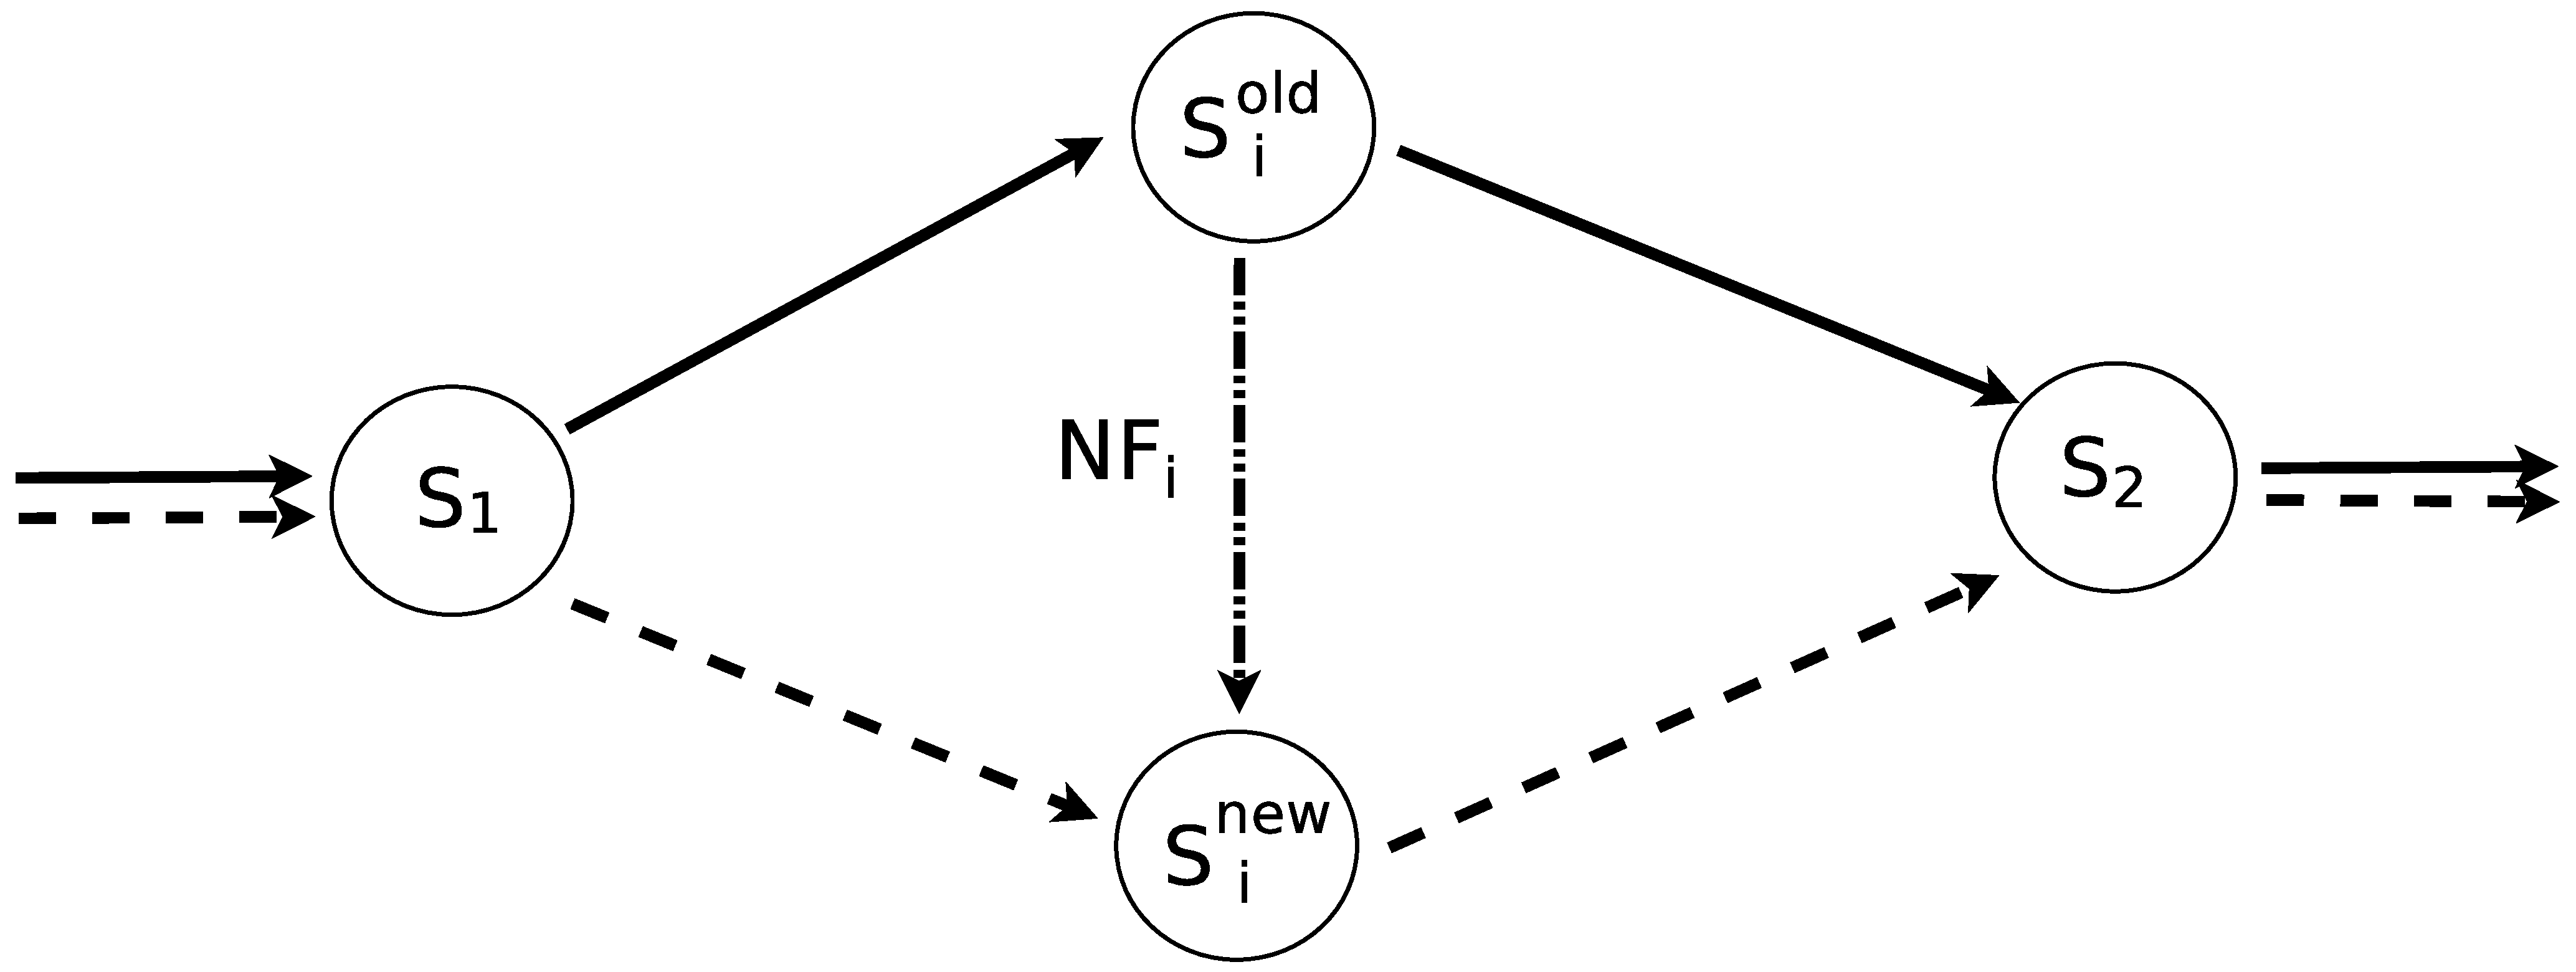
\includegraphics[width=0.85\textwidth]{basicExample.eps}
\vspace{-0.3cm}
\caption{Example of NF migration}
\label{fig:nfexample}
\vspace{-0.5cm}
\end{figure}

To understand the challenges in permitting migration alongside route
updates, consider a network function \nfID{\nfIdx} that migrates from
the old position \oldSwitchID{\nfIdx} to the new position
\newSwitchID{\nfIdx}, shown in \figref{fig:nfexample}.  The flow \flowID{}, which should be processed
by \nfID{\nfIdx}, also needs its path to be updated from $\switchID{1}
\rightarrow \oldSwitchID{\nfIdx} \rightarrow \switchID{2}$ to
$\switchID{1} \rightarrow \newSwitchID{\nfIdx} \rightarrow
\switchID{2}$. The path change can be accomplished by updating the
rule matched to \flowID{} at \switchID{1}. Migrating \nfID{\nfIdx} and
updating the path of \flowID{} without coordination can be harmful,
however. For example, if the controller sends commands to migrate
\nfID{\nfIdx} and updates \switchID{1} simultaneously, \switchID{1}
might be updated before \nfID{\nfIdx} migrates to
\newSwitchID{\nfIdx}. Then, packets of \flowID{} might start to arrive
at \newSwitchID{\nfIdx} before \nfID{\nfIdx} can process packets
there, which may cause problems since packets can bypass
\nfID{\nfIdx}. Also, if \switchID{1} has not been updated by the time
\nfID{\nfIdx} leaves \oldSwitchID{\nfIdx}, packets may arrive at
\oldSwitchID{\nfIdx} with \nfID{\nfIdx} no longer there; depending on
how \oldSwitchID{\nfIdx} handles these packets, this could result in
packet loss or packets bypassing \nfID{\nfIdx}.

Our goal is to migrate NFs and update routing-policies efficiently
while ensuring packets are processed by NFs correctly.  Specifically,
our contribution here is an algorithm that leverages consistency
properties of underlying routing-update algorithms to permit NFs to be
migrated \textit{alongside} rule deployment for new routing policies,
more efficiently than simply serializing routing-policy update after
NF migration.  In particular, our approach demonstrates that by
leveraging an SDN routing-policy update algorithm that provides a
property that we call \textit{relaxed waypoint correctness} (see
\secref{sec:schedule:condition}), we can implement waypoint
correctness when NFs are allowed to change locations much more
efficiently than known approaches to achieving both.

\subsection{Component Changes}
\label{sec:migration:components}

To support NF migration, we require that the controller, switches, and
rules be functionally enhanced in the following ways.  Below we refer
to each NF being hosted at a switch; this hosting could be implemented
on the switch for a simple NF or at an attached middlebox for a more
complex one.

\begin{figure}
\centering
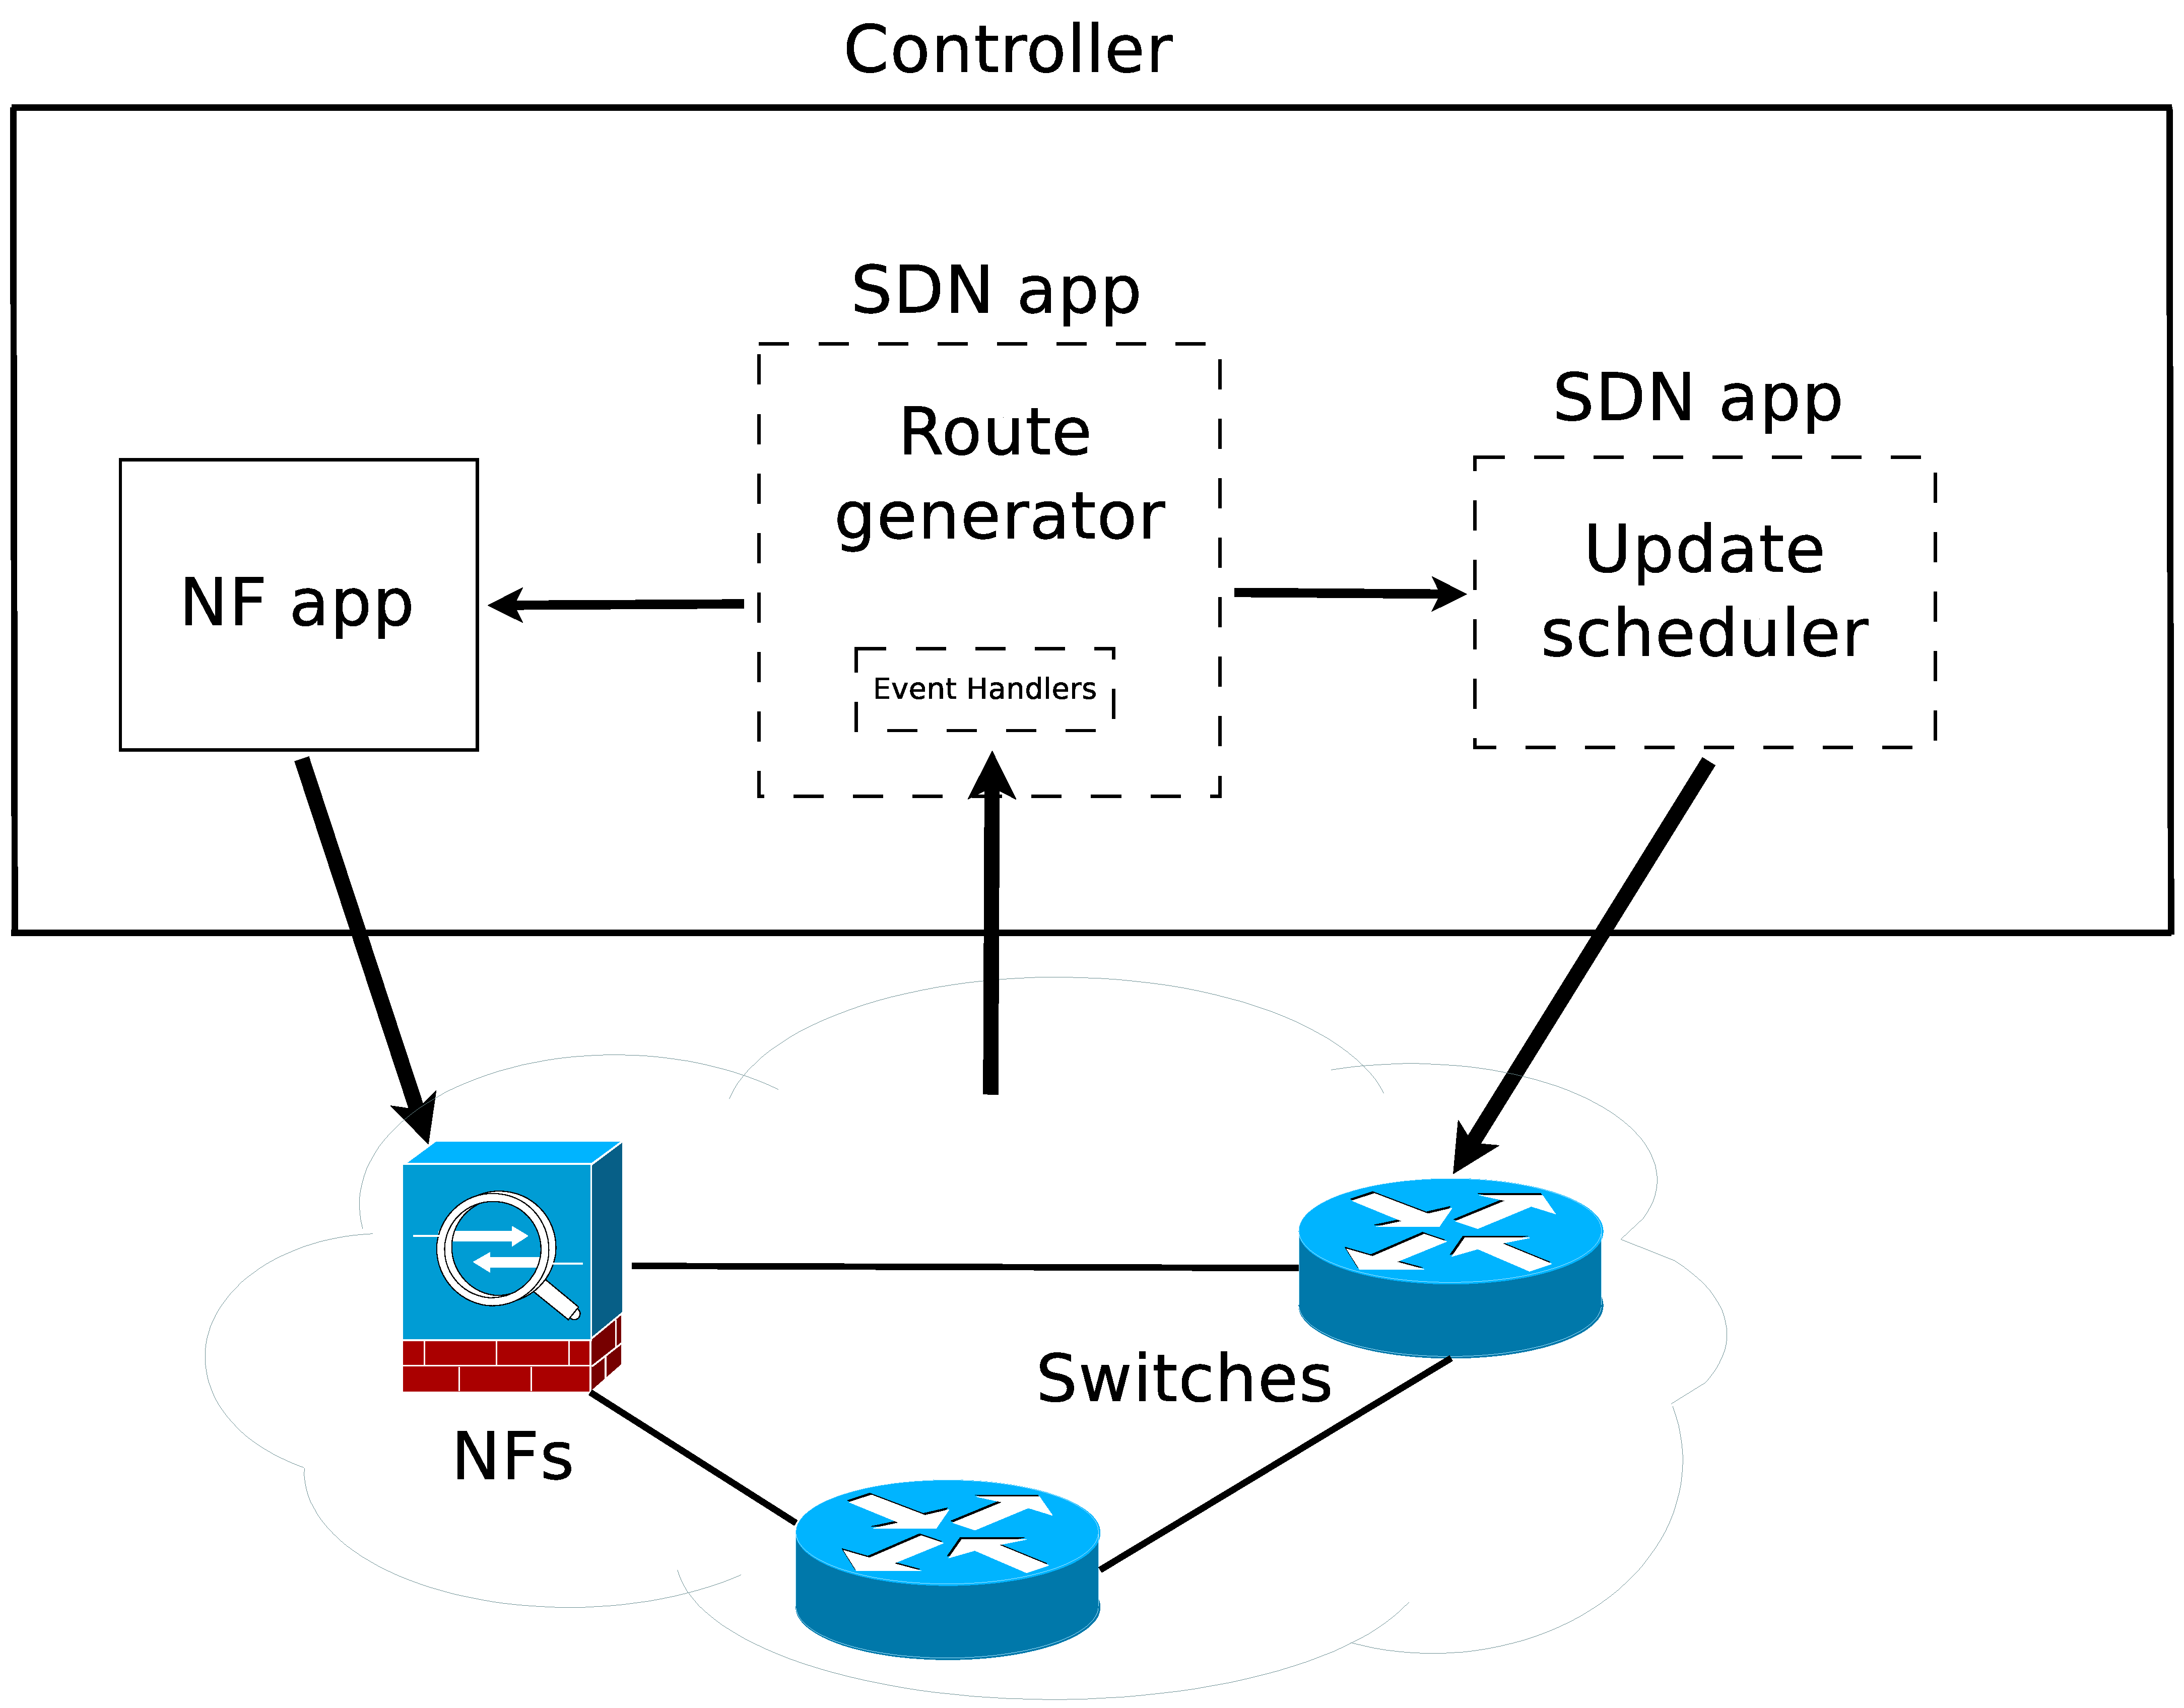
\includegraphics[width=0.8\columnwidth]{system.eps}
%\vspace{-0.3cm}
\caption{Typical components of a network controller}
\label{fig:architecture}
%\vspace{-0.5cm}
\end{figure}


\paragraph{Controller} The output from the route generator is also
provided to an NF application (see \figref{fig:architecture}), to
determine for each flow \flowID{} the switch at which \flowID{} will
be processed by each of its waypoint NFs; each NF will need to be
migrated to its corresponding switch as determined by the NF
application. It is necessary to assume that there is at least one
switch \switchID{} such that for every $\flowID{} \in
\nfID{\nfIdx}{}{\flowSpec}$, \switchID{} is included in the path of
\flowID{}, as else there is no switch to where \nfID{\nfIdx} can be
migrated to process every flow in \nfID{\nfIdx}{}{\flowSpec}.

\paragraph{Switches} We add three new switch interfaces to perform NF migration. 
\begin{itemize}[nosep,leftmargin=1em,labelwidth=*,align=left]
\item \switchID{}{\export{\nfIdx}{\switchIdx}} marshals \nfID{\nfIdx}
  into a set \pktSet of packets with source address (the IP address)
  of \switchID{} and destination address of \switchID{\switchIdx}, and
  outputs \pktSet.  \switchID{}{\export{\nfIdx}{\switchIdx}} executes
  only while no \nfID{\nfIdx}{}{\processPkt} invocations are underway
  at \switchID{}, and \switchID{} no longer permits invocations of
  \nfID{\nfIdx}{}{\processPkt} once
  \switchID{}{\export{\nfIdx}{\switchIdx}} completes.
\item \switchID{}{\import{\nfIdx}{\switchIdx}} instructs switch
  \switchID{} to await the arrival of packets \pktSet from
  \switchID{\switchIdx}, from which to reconstitute function
  \nfID{\nfIdx} locally.  This invocation causes \switchID{\switchIdx}
  to allocate two buffers, an \textit{inbound} buffer to hold packets
  to be processed in \nfID{\nfIdx}{}{\processPkt} invocations once
  \nfID{\nfIdx}{} is reconstituted locally, and an \textit{outbound}
  buffer to hold packets output from \nfID{\nfIdx}{}{\processPkt}
  invocations.  Starting from this invocation and until \nfID{\nfIdx}
  is reconstituted locally, packets matched to any $\ruleID{} \in
  \switchID{}{\ruleSet}$ for which $\ruleID{}{\sendToField} =
  \nfID{\nfIdx}{}$ (see below) are buffered in the inbound buffer for
  \nfID{\nfIdx}{}.  Packets output from \nfID{\nfIdx}{}{\processPkt}
  invocations are buffered in the outbound buffer for \nfID{\nfIdx},
  until a \switchID{}{\release{\nfIdx}} invocation.
\item \switchID{}{\release{\nfIdx}} releases the packets buffered in
  the outbound buffer for \nfID{\nfIdx} to be matched against
  \switchID{}{\ruleSet}, and disables buffering so that packets
  inbound to or outbound from \nfID{\nfIdx}{} are no longer buffered.
\end{itemize}
\switchID{}{\import}, \switchID{}{\export}, and \switchID{}{\release}
can be invoked by the controller, just like \switchID{}{\flowAdd} and
\switchID{}{\flowDel}.

\iffalse
\highlight{For example, if \nfID{2} needs to be migrated from \switchID{3} to \switchID{6}, the controller should first issue \switchID{6}{\import{2}{3}} to command \switchID{6} to wait for messages from \switchID{3}. 
Then the controller leverages the interface \switchID{3}{\export{2}{6}} to instruct \switchID{3} to create a set of packets to marshal \nfID{2} and send these packets to \switchID{6}. Upon receiving packets from \switchID{3}, \switchID{6} reconstructs \nfID{2} and starts to perform \nfID{2}{}{\processPkt} invocations. Finally, after new routing policy is enabled, the controller can issue \switchID{6}{\release{2}} command and \switchID{6} releases the buffered packets to the network.}
\fi

\paragraph{Waypoint counters}  We add to each packet a field, called its
\textit{waypoint counter}, that can hold any value in
$\nats{\wpNmbrMax+1} = \{1, \ldots, \wpNmbrMax+1\}$.  Upon arrival in
the network, a packet's ingress switch initializes the packet's
waypoint counter to $1$.  In brief, this counter is incremented in the
packet as it is submitted to each of its waypoints for processing (see
below).  In this way, rules can treat a packet differently depending
on how many of its waypoints it has already traversed.

\paragraph{Rules} We extend rules to include a new field
\ruleID{}{\wpField} that takes on a value in $\nats{\wpNmbrMax} \cup
\{\ast\}$, and stipulate that a packet can be matched to this rule
only if $\ruleID{}{\wpField} = \ast$ or the packet's waypoint counter
equals \ruleID{}{\wpField}.  As such, when packet \pktID{} in flow
\flowID{} arrives at switch \switchID{}, \pktID{} is matched to the
highest priority rule $\ruleID{} \in \switchID{}{\ruleSet}$ for which
$\flowID{} \in \ruleID{}{\coverField}$ and either $\ruleID{}{\wpField}
= \ast$ or the packet's waypoint counter equals \ruleID{}{\wpField};
we denote this rule as \ruleMatchNew{\switchID{}}{\pktID{}}.  If there is
no $\ruleID{} \in \switchID{}{\ruleSet}$ to which \pktID{} can be
matched, then \pktID{} is dropped.

We also extend rules to accommodate additional functionality
related to the \ruleID{}{\sendToField} field.
\begin{itemize}[nosep,leftmargin=1em,labelwidth=*,align=left]
\item \ruleID{}{\sendToField} can be a network function \nfID{\nfIdx},
  in which case for any packet \pktID{} it matches to \ruleID{},
  $\switchID{} = \ruleID{}{\switchField}$ increments the \pktID{}'s
  waypoint counter and then submits \pktID{} to \nfID{\nfIdx} in an
  \nfID{\nfIdx}{}{\processPkt{\pktID{}}} invocation.  If
  \nfID{\nfIdx}{} is not hosted locally at \ruleID{}{\switchField{}},
  then the packet must be buffered (in the inbound buffer for
  \nfID{\nfIdx}, see above) until it is.  Any packets returned from
  the \nfID{\nfIdx}{}{\processPkt{\pktID{}}} invocation are matched
  again to \switchID{}{\ruleSet}.  We do not require \nfID{\nfIdx} to
  process packets' waypoint counters, but we do require that any
  packets \nfID{\nfIdx}{}{\processPkt{\pktID{}}} emits bear
  the same waypoint counter as \pktID{}.
\item \ruleID{}{\sendToField} can take on two more possible values,
  namely functions \encapsulate{\flowID{}} and \decapsulate.  If a
  switch \switchID{} matches packet \pktID{} to rule $\ruleID{} \in
  \switchID{}{\ruleSet}$ where $\ruleID{}{\sendToField} =
  \encapsulate{\flowID{}}$, then the packet is encapsulated into a
  packet for flow \flowID{}, which is then resubmitted for matching
  against \switchID{}{\ruleSet} at this switch \switchID{}.  A packet
  matched to a rule $\ruleID{} \in \switchID{}{\ruleSet}$ where
  $\ruleID{}{\sendToField} = \decapsulate$ is decapsulated (i.e., the
  existing packet header is removed) and the packet contained therein
  is then resubmitted for matching against \switchID{}{\ruleSet}.
\end{itemize}
As before, all rule fields remain immutable.
\iffalse
\highlight{For example, \switchID{1} is the new location for \nfID{2} and has rules \ruleID{1}, \ruleID{2}, \ruleID{3}.
\flowID{1} matches to \ruleID{1} and $\ruleID{1}{\sendToField} = \decapsulate$. \ruleID{2} satisfies that $\flowID{2} \in \ruleID{2}{\coverField}$, $\ruleID{2}{\wpField} = 3$ and $\ruleID{2}{\sendToField} = \nfID{2}$.
\ruleID{3} satisfies that $\flowID{2} \in \ruleID{3}{\coverField}$, $\ruleID{3}{\wpField} = \ast$ and $\ruleID{3}{\sendToField} = \switchID{2}$. \ruleID{2} is of higher priority than \ruleID{3}, i.e., $\ruleID{2}{\priorityField} > \ruleID{3}{\priorityField}$. Say \switchID{1} receives a packet \pktID{1} of \flowID{1}. \switchID{1} decapsulates \pktID{1} to \pktID{2} of \flowID{2}, since \pktID{1} matches to \ruleID{1}. Assume \pktID{2} carries waypoint counter $3$. Then \switchID{1} resubmits \pktID{2} to the rule table and executes the action of \ruleID{2}. \pktID{2} is sent to \nfID{2} and its waypoint counter is increased to $4$. Therefore, when \switchID{1} processes \pktID{2} again, \pktID{2} matches to \ruleID{3} and is forwarded to \switchID{2}.
}
\fi

\subsection{Algorithm}
\label{sec:migration:algo}

\begin{figure}[t]
\centering
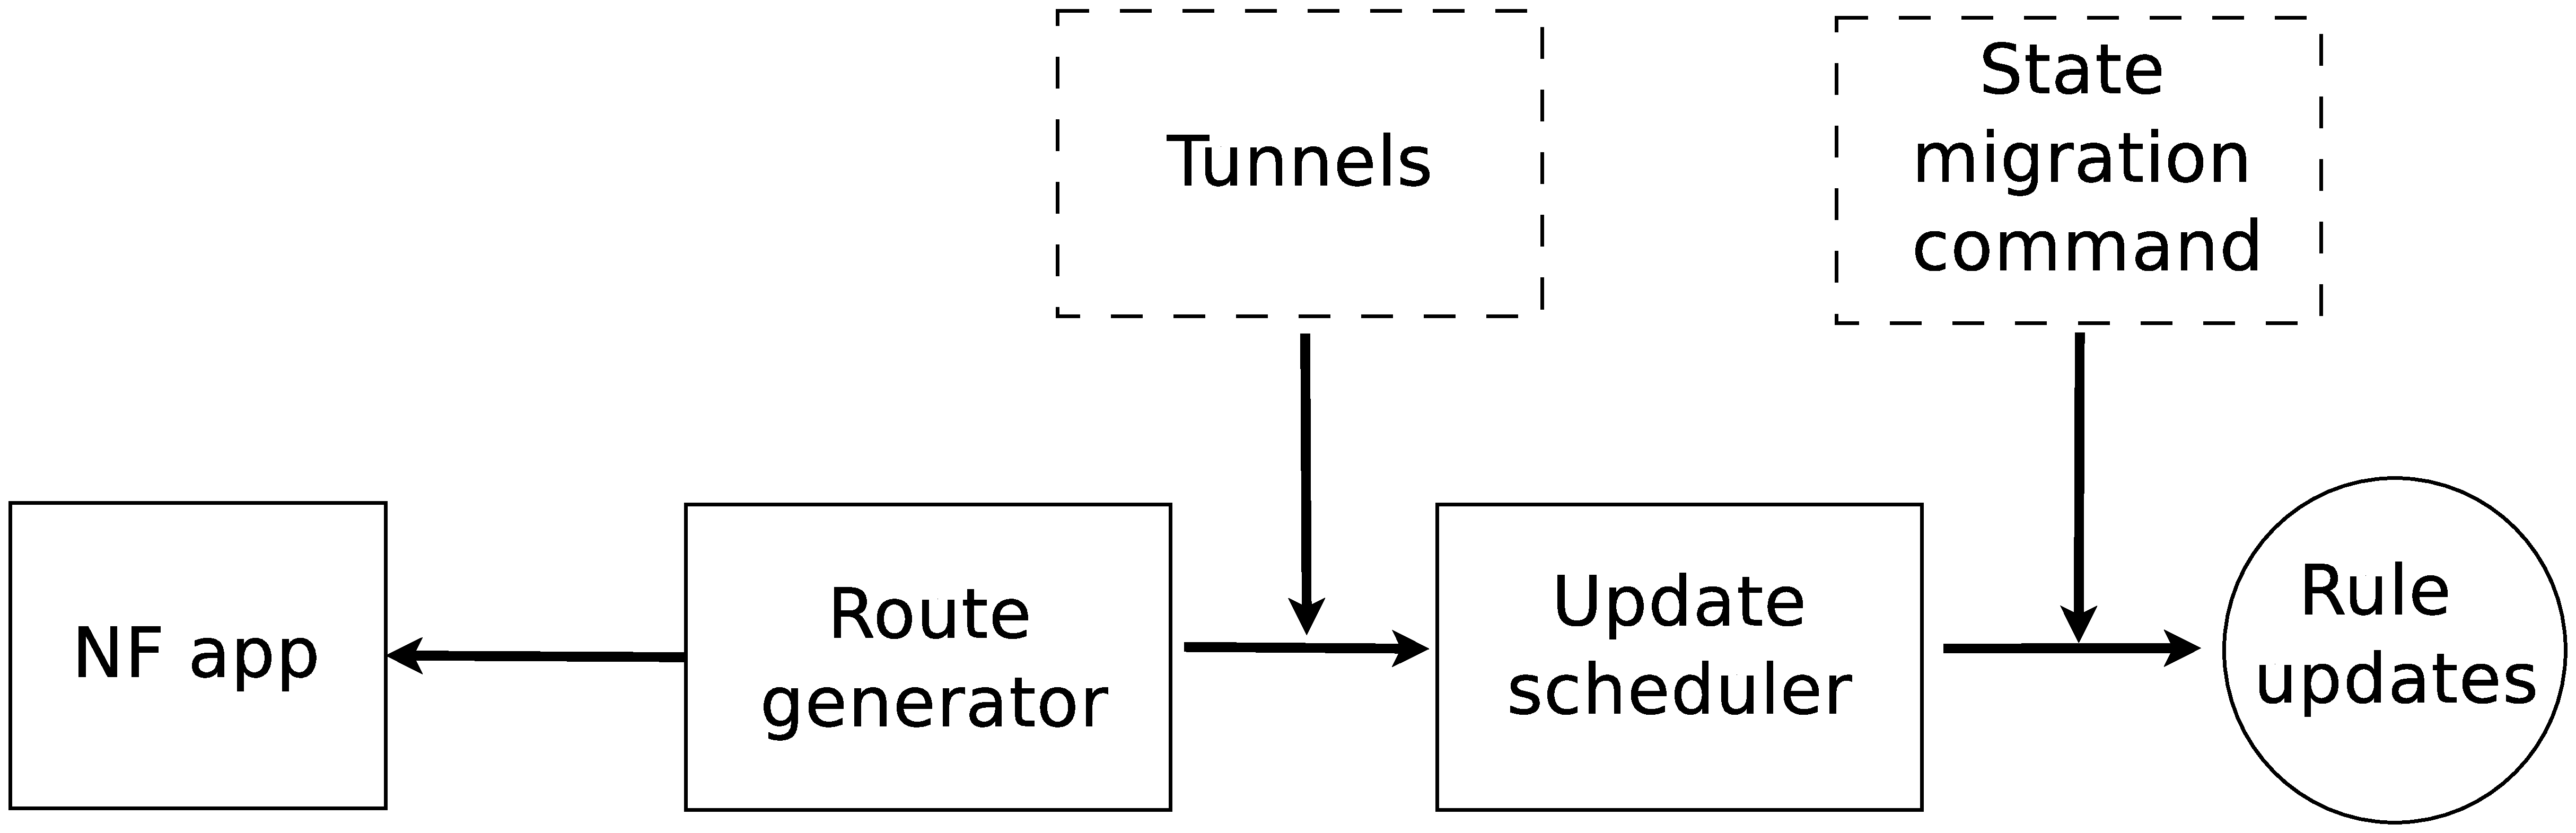
\includegraphics[width=0.9\textwidth]{algorithm.eps}
\caption{Conceptual additions by our algorithm}
\label{fig:algorithm}
\vspace{-0.3cm}
\end{figure}

Our algorithm augments the SDN framework outlined in
\secref{sec:goals} with two conceptual steps (see
\figref{fig:algorithm}).  The first instantiates routing policy for
tunnels to migrate NFs from their old locations to their new locations
and to relocate traffic that arrives at an NF's old location to its
new location.  Once these routes have been determined, the full
routing policy (including these new routes) is then submitted to the
routing-policy update scheduler, which produces the schedule for
deploying rules to switches.  The second phase of our algorithm then
augments this update schedule with commands to bridge traffic on/off
of tunnels as needed, to invoke each NF with packets destined for it
at its new location, and to initiate migration of NFs.  A later phase
of our algorithm (not shown in \figref{fig:algorithm}) cleans up the
bridging rules once they are no longer needed.



The first of these steps is implemented as follows, per \nfID{\nfIdx}
that migrates from \oldSwitchID{\nfIdx} to \newSwitchID{\nfIdx} in
this epoch.

\hspace*{-\parindent}
\fbox{\begin{minipage}[t]{0.95\columnwidth}
\textbf{Migration routes}: The controller constructs a route from
\oldSwitchID{\nfIdx} to \newSwitchID{\nfIdx} to carry flows
\flowIDMigrate{\nfIdx}, \flowIDTunnel{\nfIdx} with source
\oldSwitchID{\nfIdx} and destination \newSwitchID{\nfIdx}.
\flowIDMigrate{\nfIdx}, \flowIDTunnel{\nfIdx} and their associated
route are added to the routing policy that is input to the update
scheduler.
\end{minipage}}

\flowIDMigrate{\nfIdx} will be used to migrate \nfID{\nfIdx} from
\oldSwitchID{\nfIdx} to \newSwitchID{\nfIdx}, and
\flowIDTunnel{\nfIdx} will be used to tunnel packets from
\oldSwitchID{\nfIdx} to \newSwitchID{\nfIdx} that should be processed
by \nfID{\nfIdx}.  Because we assume that the IP addresses of
\oldSwitchID{\nfIdx} and \newSwitchID{\nfIdx} are distinct from the
source and destination addresses of flows routed according to the
policies output from the route generator, the routes chosen to carry
\flowIDMigrate{\nfIdx}, \flowIDTunnel{\nfIdx} cannot contradict the
routes output from the route generator.

\figref{fig:algorithmExample} shows an example for this step.  Suppose
a flow \flowID{} which is processed by \nfID{1} and \nfID{2} needs to
be rerouted from the path $\switchID{1} \rightarrow \switchID{2}
\rightarrow \switchID{3} \rightarrow \switchID{4} \rightarrow
\switchID{5} \rightarrow \switchID{6}$ (solid line) to the path
$\switchID{1} \rightarrow \switchID{7} \rightarrow \switchID{4}
\rightarrow \switchID{8} \rightarrow \switchID{9} \rightarrow
\switchID{6}$ (dash line).  And consequently, the controller decides
to migrate \nfID{1} from \switchID{2} ($= \oldSwitchID{1}$) to
\switchID{7} ($= \newSwitchID{1}$) and \nfID{2} from \switchID{3} ($=
\oldSwitchID{2}$) to \switchID{9} ($= \newSwitchID{2}$).
$\switchID{2} \rightarrow \switchID{1} \rightarrow \switchID{7}$ can
be selected for migration route between \oldSwitchID{1} and
\newSwitchID{1}. $\switchID{3} \rightarrow \switchID{4} \rightarrow
\switchID{8} \rightarrow \switchID{9}$ can be selected for migration
route between \oldSwitchID{2} and \newSwitchID{2}.

\begin{figure}
\centering
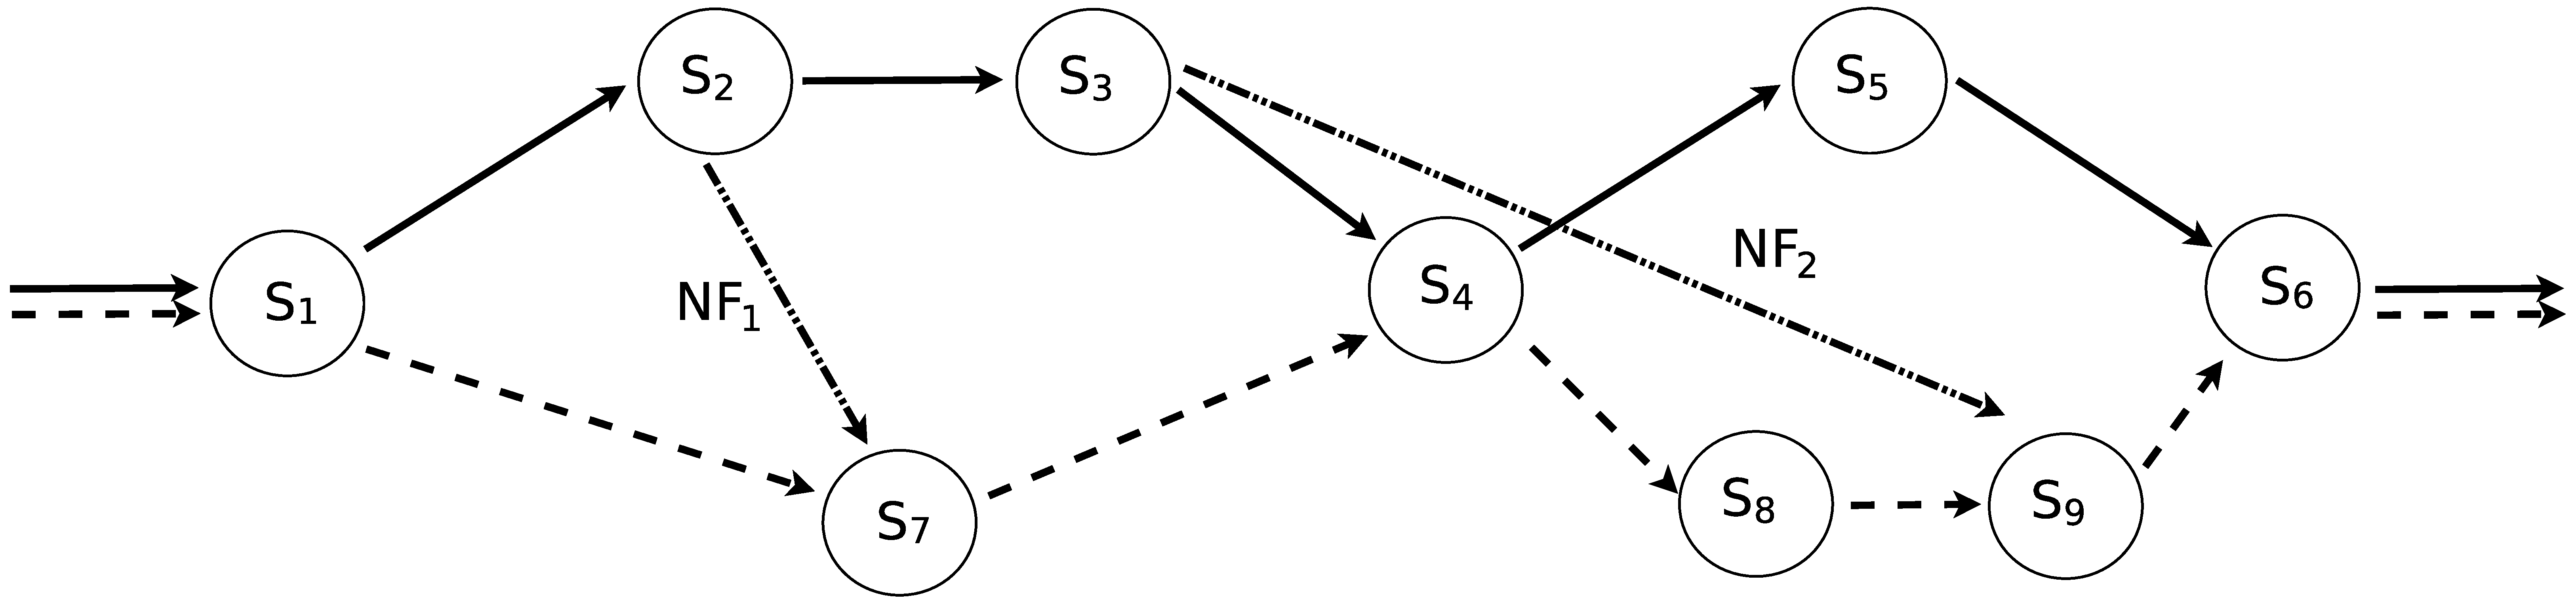
\includegraphics[width=0.95\columnwidth]{algorithmExample.eps}

\caption{Example for algorithm description}
\label{fig:algorithmExample}
\end{figure}

Recall that the update generator now outputs a schedule for rule
deployment in \updateSteps steps $\updateID{1}, \updateID{2}, \ldots,
\updateID{\updateSteps}$, where each \updateID{\updateIdx} includes a
set of \flowAdd and \flowDel commands.  Continuing with the example of
\figref{fig:algorithmExample}, to ensure that packets cannot bypass
waypoints, the update scheduler might formulate the following
three-step schedule.  In the first step, \switchID{7}, \switchID{8},
and \switchID{9} install new rules; i.e., \updateID{1} should include
the flow modification commands for these three switches.  In the
second step (\updateID{2}), \switchID{4} is updated to send packets to
\switchID{8}.  In the third step (\updateID{3}), \switchID{1} is
modified and packets are sent through the new path.  Recall that these
update steps include commands output by the update scheduler to
install rules to route the tunnels generated in the previous step of
our algorithm.

Continuing our algorithm, it first sets $\ruleID{}{\wpField} \gets
\ast$ for any rule \ruleID{} in any \flowAdd or \flowDel command
in any step of the given update schedule $\updateID{1}, \ldots,
\updateID{\updateSteps}$.  Then, for each \nfID{\nfIdx} to be hosted
at a switch \newSwitchID{\nfIdx} in this epoch different from the
switch \oldSwitchID{\nfIdx} where it was hosted in the last, the
controller performs the following steps.

\hspace*{-\parindent} \fbox{\begin{minipage}[t]{0.95\columnwidth}
    \textbf{Rules for routing to \nfID{\nfIdx}}: The controller constructs
    $\wpNmbrMax+2$ rules as follows.  First, the controller constructs
    a rule \ruleIDIn{\nfIdx} with the following fields:
\begin{itemize}[nosep,leftmargin=1em,labelwidth=*,align=left]
  \item $\ruleIDIn{\nfIdx}{\switchField} \gets \oldSwitchID{\nfIdx}$
  \item $\ruleIDIn{\nfIdx}{\coverField} \!\gets\!
    \left\{\flowID{} ~\left|~\!
    \begin{array}{@{}r@{\hspace{0.25em}}r@{}}
      \exists \pktID{}, \ruleID{}: & \pktID{} \in \flowID{} \\
      \wedge & \ruleID{} \in \oldSwitchID{\nfIdx}{\ruleSet} \\
      \wedge & \ruleID{} = \ruleMatchNew{\oldSwitchID{\nfIdx}}{\pktID{}}\\
      \wedge & \ruleID{}{\sendToField} = \nfID{\nfIdx}
    \end{array}
    \right.
    \right\}$
  \item $\ruleIDIn{\nfIdx}{\wpField} \gets \ast$
  \item $\ruleIDIn{\nfIdx}{\priorityField} \gets \infty$
  \item $\ruleIDIn{\nfIdx}{\sendToField} \gets
    \encapsulate{\flowIDTunnel{\nfIdx}}$
\end{itemize}
In addition, the controller constructs the rule \ruleIDOut{} with
the following fields:
\begin{itemize}[nosep,leftmargin=1em,labelwidth=*,align=left]
  \item $\ruleIDOut{\nfIdx}{\switchField} \gets \newSwitchID{\nfIdx}$
  \item $\ruleIDOut{\nfIdx}{\coverField} \gets \{\flowIDTunnel{\nfIdx}\}$
  \item $\ruleIDOut{\nfIdx}{\wpField} \gets \ast$
  \item $\ruleIDOut{\nfIdx}{\priorityField} \gets \infty$
  \item $\ruleIDOut{\nfIdx}{\sendToField} \gets \decapsulate$
\end{itemize}
Finally, for each $\wpIdx \in \nats{\wpNmbrMax}$, the controller
constructs a rule \ruleIDInv{\nfIdx}{\wpIdx} with the following
fields:
\begin{itemize}[nosep,leftmargin=1em,labelwidth=*,align=left]
  \item $\ruleIDInv{\nfIdx}{\wpIdx}{\switchField} \gets \newSwitchID{\nfIdx}$
  \item $\ruleIDInv{\nfIdx}{\wpIdx}{\coverField} \gets \{\flowID{} \mid \wpFn{\flowID{}}{\wpIdx} = \nfIdx\}$
  \item $\ruleIDInv{\nfIdx}{\wpIdx}{\wpField} \gets \wpIdx$
  \item $\ruleIDInv{\nfIdx}{\wpIdx}{\priorityField} \gets \infty$
  \item $\ruleIDInv{\nfIdx}{\wpIdx}{\sendToField} \gets \nfID{\nfIdx}$
\end{itemize}
\end{minipage}}

In the example of \figref{fig:algorithmExample}, \switchID{2} and
\switchID{3} should install rule \ruleIDIn{1} and \ruleIDIn{2},
respectively, to encapsulate packets of \flowID{} onto
\flowIDTunnel{\nfIdx}.  In this way, packets arriving at \switchID{2}
or \switchID{3} can be relocated to new positions \switchID{7} and
\switchID{9}, respectively, during NF migration. Packets relocated
through these tunnels to the new NF locations should be decapsulated
back to the original flow \flowID{} such that they can traverse the
remainder of the new path after being processed by the appropriate
NF. Therefore, \switchID{7} and \switchID{9} need rules \ruleIDOut{1}
and \ruleIDOut{2}, respectively.

\ruleIDInv{\nfIdx}{\wpIdx} has two functions. First, it sends packets
that need to be processed (i.e., with waypoint counter \wpIdx where
$\wpFn{\flowID{}}(\wpIdx) = \nfIdx$) to \nfID{\nfIdx}.  Note that
packets on \flowID{} output from \nfID{\nfIdx} will have a waypoint
counter of $\wpIdx+1$ and thus will not be matched to
\ruleIDInv{\nfIdx}{\wpIdx} again.  Second, \ruleIDInv{\nfIdx}{\wpIdx}
prevents packets from being processed twice by \nfID{\nfIdx}.
Continuing with the example of \figref{fig:algorithmExample}, since at
the beginning of $\updateID{3}$, \switchID{4} has been updated (in
\updateID{2}) but \switchID{1} has not yet been changed, packets on
\flowID{} traversing a part of old path ($\switchID{1} \rightarrow
\switchID{2} \rightarrow \switchID{3} \rightarrow \switchID{4}$) and a
part of new path ($\switchID{4} \rightarrow \switchID{8} \rightarrow
\switchID{9} \rightarrow \switchID{6}$) encounter both the old
(\switchID{3}) and new position (\switchID{9}) of \nfID{2}.
$\ruleIDInv{2}{2}$ at \switchID{9} ensures packets carrying waypoint
counter $2$ can be processed by \nfID{2}, but packets with waypoint
counter $3$ (\nfID{2} already processed these packets at \switchID{3})
are forwarded to next switch \switchID{6} immediately.

Now that these rules have been generated, we need to integrate them
into the update schedule.  To do so, the algorithm initializes
\updateID{\updateSteps+1} to be empty, i.e.,
$\updateID{\updateSteps+1} \gets \{\}$.  Then, for each migrating
network function \nfID{\nfIdx}, the controller performs the following.

\hspace*{-\parindent}
\fbox{\begin{minipage}[t]{0.95\columnwidth}
\textbf{Update schedule}: To deploy \ruleIDIn{\nfIdx},
\ruleIDOut{\nfIdx}, $\{\ruleIDInv{\nfIdx}{\wpIdx}\}_{\wpIdx \in
  \nats{\wpNmbrMax}}$ in the update schedule \updateID{1},
\updateID{2}, $\ldots$, \updateID{\updateSteps+1}, the controller
performs the following steps.
\begin{itemize}[nosep,leftmargin=1em,labelwidth=*,align=left]
  \item The controller adds
    \newSwitchID{\nfIdx}{\flowAdd{\ruleIDOut{\nfIdx}}},
    \newSwitchID{\nfIdx}{\import{\nfIdx}{\switchIdx}}, and
    \newSwitchID{\nfIdx}{\flowAdd{\ruleIDInv{\nfIdx}{\wpIdx}}} for
    each $\wpIdx \in \nats{\wpNmbrMax}$ to \updateID{1},
    where $\oldSwitchID{\nfIdx} = \switchID{\switchIdx}$.
  \item The controller searches for the last step
    \updateID{\updateIdx} in which rules to route
    \flowIDMigrate{\nfIdx}, \flowIDTunnel{\nfIdx} are deployed.  It
    adds \oldSwitchID{\nfIdx}{\flowAdd{\ruleIDIn{\nfIdx}}} and
    \oldSwitchID{\nfIdx}{\export{\nfIdx}{\switchIdx}} to
    \updateID{\updateIdx+1} where $\newSwitchID{\nfIdx} =
    \switchID{\switchIdx}$.
  \item The controller adds \newSwitchID{\nfIdx}{\release{\nfIdx}} to
    \updateID{\updateSteps+1}.
  \end{itemize}
\end{minipage}}

The first bullet incorporates commands to prepare switches at new
positions for NF migration. 
In the example of \figref{fig:algorithmExample}, the controller issues commands \switchID{7}{\import{1}{2}}, \switchID{7}{\flowAdd{\ruleIDOut{1}}} and \switchID{7}{\flowAdd{\ruleIDInv{1}{1}}} to \switchID{7}. So \switchID{7} waits for messages from \switchID{2} and prepares to reconstruct \nfID{1} locally. The controller also performs similar operations on \switchID{9}.

The second bullet incorporates commands to migrate \nfID{\nfIdx} from its old to its new
position. This should be done after the rules implementing the
migration route have been deployed (i.e., after step
$\updateID{\updateIdx}$). 
In the example of \figref{fig:algorithmExample}, assume the controller deploys rules to create a tunnel $\switchID{2} \rightarrow \switchID{1} \rightarrow \switchID{7}$ to migrate \nfID{1} from \switchID{2} to \switchID{7} in step \updateID{1}. Then, in step \updateID{2}, the controller can use the interface \switchID{2}{\export{1}{7}} to instruct \switchID{2} to create a set of packets to marshal \nfID{1} and send these packets to \switchID{7}. Upon receiving packets from \switchID{2}, \switchID{7} reconstructs \nfID{1} and starts to perform \nfID{1}{}{\processPkt} invocations. Meanwhile, \switchID{2} uses the rule \ruleIDIn{1} to encapsulate the packets of \flowID{} to packets of \flowIDTunnel{1}. Packets of \flowIDTunnel{1} are then forwarded to \switchID{7} and \switchID{7} uses the rule \ruleIDOut{1} to decapsulate these packets back to packets of \flowID{}. The packets have not been processed by \switchID{2} and therefore should carry the waypoint counter $1$. Thus, \switchID{7} uses the rule \ruleIDInv{1}{1} to forward packets to \nfID{1}. After processed by \nfID{1}, these packets are buffered at \switchID{7} with the waypoint counter $2$.

The last bullet ensures that packets
released from switches at new positions can be matched to rules
implementing new routing policy at all downstream switches.
In the example of \figref{fig:algorithmExample}, the controller sends \switchID{7}{\release{1}} in step \updateID{4}. \switchID{7} then releases the buffered packets to the network since \switchID{4}, \switchID{8} and \switchID{9} have installed rules to forward packets to the destination.

The last step of our algorithm cleans up migration-related rules once
they will no longer be used.  Specifically, for each migrated
\nfID{\nfIdx}, the following is performed:

\hspace*{-\parindent}
\fbox{\begin{minipage}[t]{0.95\columnwidth}
\textbf{Bridging rules cleanup}: After sufficient time passes to
ensure that \flowIDMigrate{\nfIdx} and \flowIDTunnel{\nfIdx} will
contain no more packets, the controller issues
\oldSwitchID{\nfIdx}{\flowDel{\ruleIDIn{\nfIdx}}} and
\newSwitchID{\nfIdx}{\flowDel{\ruleIDOut{\nfIdx}}} commands.
\end{minipage}}

In \figref{fig:algorithmExample}, this step causes the deletion of
\ruleIDIn{1} and \ruleIDOut{1} from \switchID{2} and \switchID{7},
respectively, and the deletion of \ruleIDIn{2} and \ruleIDOut{2} from
\switchID{3} and \switchID{9}, respectively.  The rules to implement
the migration routes $\switchID{2} \rightarrow \switchID{1}
\rightarrow \switchID{7}$ and $\switchID{3} \rightarrow \switchID{4}
\rightarrow \switchID{8} \rightarrow \switchID{9}$ can also be
removed, if doing so does not disrupt other routing policy.

\section{Update Scheduling}
\label{sec:schedule}

The algorithm described in the previous section adapts a given update
schedule with additional \flowDel, \flowAdd, \export, \import, and
\release commands to migrate NFs during path updates.  In this
section, we explore the requirements for the given update schedule
that, when combined with the algorithm of the previous section,
ensures waypoint correctness as defined in
\secref{sec:goals:correctness}.  We define a sufficient condition in
\secref{sec:schedule:condition}.  Finally, in
\secref{sec:schedule:rwc} we provide an update scheduling algorithm
that is tailored to implement specifically this condition.

\subsection{A Sufficient Condition for Waypoint Correctness}
\label{sec:schedule:condition}

In this section we give a sufficient condition for the NF-migration
algorithm of \secref{sec:migration} to ensure the waypoint correctness
property defined in \secref{sec:goals:correctness}.  Recall that
during a route change, each \nfID{\nfIdx} is migrated from its old
location \oldSwitchID{\nfIdx} to its new location
\newSwitchID{\nfIdx}, while traffic to be processed by \nfID{\nfIdx}
that arrives at \oldSwitchID{\nfIdx} and matched to a rule \ruleID{}
with $\ruleID{}{\sendToField} = \nfID{\nfIdx}$ is transported from
\oldSwitchID{\nfIdx} to \newSwitchID{\nfIdx} to be processed once
\nfID{\nfIdx} is reconstituted there.  Whether traffic reaches
\newSwitchID{\nfIdx} via this mechanism or by the new routing policy
does not matter.  Rather, all that really matters is that a packet on
flow \flowID{} with waypoint counter \wpIdx reaches either
\oldSwitchID{\wpFn{\flowID{}}{\wpIdx}} or
\newSwitchID{\wpFn{\flowID{}}{\wpIdx}}.  We call this property
\textit{relaxed waypoint correctness}:

\paragraph{Relaxed waypoint correctness} An update scheduling algorithm
satisfies \textit{relaxed waypoint correctness} if during any route
update, it ensures that for each flow \flowID{} and each $\wpIdx \in
\nats{\wpNmbr{\flowID{}}}$, each packet on flow \flowID{} with
waypoint counter \wpIdx reaches \oldSwitchID{\wpFn{\flowID{}}{\wpIdx}}
or \newSwitchID{\wpFn{\flowID{}}(\wpIdx)}.\footnote{Strictly speaking,
  since a packet on flow \flowID{} has its waypoint counter
  incremented to $\wpIdx+1$ right \textit{before} processing by
  \nfID{\nfIdx} for $\nfIdx = \wpFn{\flowID{}}(\wpIdx)$, it is
  possible that this property will fail for a packet that is not then
  output from \nfID{\nfIdx} (e.g., because \nfID{\nfIdx} drops it).
  We require this property for every packet on \flowID{} output from
  \nfID{\nfIdx}, however.}

\medskip

Our NF-migration algorithm in \secref{sec:migration} guarantees the waypoint correctness property defined in \secref{sec:goals:correctness}, if the underlying update scheduling algorithm (used by the update scheduler in the controller) satisfies the relaxed waypoint correctness.
An example of an update scheduling algorithm that implements this
property is CU~\cite{CU}, which on its own ensures that each packet
traverses either the old path in its entirety or the new path in its
entirety.  When conjoined with our NF migration algorithm, a packet
that is being routed along its old path might be tunneled from
\oldSwitchID{\nfIdx} to \newSwitchID{\nfIdx} for processing by
\nfID{\nfIdx}, after which it will be buffered until the route update
is complete.  From that point forward, it will be routed along its new
path.  A natural question is whether there are route update algorithms
that satisfy relaxed waypoint correctness without enforcing a packet
to traverse only the path of its old flow or of its new one.  In
the next section we answer this question in the affirmative.

%\input{modelchecking}


\subsection{Update Scheduling for Relaxed Waypoint Correctness}
\label{sec:schedule:rwc}

In this section we provide an update scheduling algorithm, which we
call \ourRouteUpdateName (for \ourRouteUpdateNameLong), that is
specifically designed to satisfy relaxed waypoint correctness, no
more, no less, whenever it is possible to achieve this property while
updating each switch only once during an epoch change.  The algorithm
is inspired by the TSU~\cite{tsu} routing update algorithm, though we
have adapted it to accommodate NF migration and waypoint ordering.

The algorithm computes the update schedule \updateID{1}, \updateID{2},
$\ldots$, \updateID{\updateSteps} using an optimization expressed as a
0-1 integer linear program, which can be solved (if it has a solution)
using solvers like CPLEX~\cite{CPLEX} or Gurobi~\cite{gurobi}.  This algorithm assumes that the
old and new routing policies differ only in a single path; i.e., a
flow \flowID{} (or set of flows) transitions from the same old path to
the same new path.  (Multiple path changes can be implemented
one-by-one in multiple updates.)  Moreover, this algorithm assumes
that both the old and new path are loop-free.

\subsubsection{Integer program}
\label{sec:schedule:tsu:ip}

Let \oldSwitchesSet be the set of switches that appear on the old
path; \newSwitchesSet the set of switches that appear on the new path;
$\switchesSet = \oldSwitchesSet \cup \newSwitchesSet$; $\oldPathNB{}
\subseteq \oldSwitchesSet \times \oldSwitchesSet$ the links comprising
the old path; and $\newPathNB{} \subseteq \newSwitchesSet \times
\newSwitchesSet$ the links comprising the new path.  Therefore,
$\oldPathNB{} \setminus \newPathNB{}$ is the set of links that will be
\textit{disabled} by the path change (i.e., that will no longer be
traversed by the rerouted flow \flowID{}), and $\newPathNB{} \setminus
\oldPathNB{}$ is the set of links that will be \textit{enabled} by the
path change.  Let $\switchesWLinkSwapSet \subseteq \oldSwitchesSet
\cap \newSwitchesSet$ contain the switches at which links to carry
\flowID{} must be both enabled and disabled, i.e.,
$\switchID{\switchIdx} \in \switchesWLinkSwapSet$ iff
$\switchID{\switchIdx} \in \oldSwitchesSet \cap \newSwitchesSet$ and
for some \switchID{\switchIdxAlt}, $(\switchID{\switchIdx},
\switchID{\switchIdxAlt}) \in (\oldPathNB{} \setminus \newPathNB{}) \cup
(\newPathNB{} \setminus \oldPathNB{})$.  Let \enableLinksSet be the new links
enabled at the switches in \switchesWLinkSwapSet, and let
\disableLinksSet bet the old links disabled at the switches in
\switchesWLinkSwapSet; i.e., $(\switchID{\switchIdx},
\switchID{\switchIdxAlt}) \in \enableLinksSet$ iff
$\switchID{\switchIdx} \in \switchesWLinkSwapSet$ and
$(\switchID{\switchIdx}, \switchID{\switchIdxAlt}) \in \newPathNB{}
\setminus \oldPathNB{}$, and $(\switchID{\switchIdx},
\switchID{\switchIdxAlt}) \in \disableLinksSet$ iff
$\switchID{\switchIdx} \in \switchesWLinkSwapSet$ and
$(\switchID{\switchIdx}, \switchID{\switchIdxAlt}) \in \oldPathNB{}
\setminus \newPathNB{}$.  For a natural number \genericNat, let
$\nats{\genericNat} = \{1, \ldots, \genericNat\}$.


\begin{figure*}[t]
\centering
\noindent
\fbox{\begin{minipage}{0.95\linewidth}
  
  \begin{align}
    \mathclap{\mbox{Minimize } \updateStepsAlt \mbox{ subject to:}}
    \label{eqn:update:goal} \\
    \updateStepsAlt & \geq \updateIdx \cdot \switchUpdateInd{\updateIdx}{\switchIdx}
    & \forall \updateIdx \in \nats{\switchNmbr}, \switchID{\switchIdx} \in \switchesWLinkSwapSet
    \label{eqn:update:roundBound} \\
    1 & = \sum_{\updateIdx \in \nats{\switchNmbr}} \switchUpdateInd{\updateIdx}{\switchIdx}
    & \forall \switchID{\switchIdx} \in \switchesWLinkSwapSet
    \label{eqn:update:oneChange} \\
    \linkActiveInd{\updateIdx}{\switchIdx}{\switchIdxAlt} & = 1 - \sum_{\updateIdxAlt \leq \updateIdx} \switchUpdateInd{\updateIdxAlt}{\switchIdx}
    & \forall \updateIdx \in \nats{\switchNmbr}, (\switchID{\switchIdx}, \switchID{\switchIdxAlt}) \in \disableLinksSet
    \label{eqn:update:disableLinks} \\
    \linkActiveInd{\updateIdx}{\switchIdx}{\switchIdxAlt} & = \sum_{\updateIdxAlt \leq \updateIdx} \switchUpdateInd{\updateIdxAlt}{\switchIdx}
    & \forall \updateIdx \in \nats{\switchNmbr}, (\switchID{\switchIdx}, \switchID{\switchIdxAlt}) \in \enableLinksSet
    \label{eqn:update:enableLinks} \\
    \linkActiveInd{\updateIdx}{\switchIdx}{\switchIdxAlt} & = 1
    & \forall \updateIdx \in \nats{\switchNmbr},
    (\switchID{\switchIdx}, \switchID{\switchIdxAlt}) \in
    (\oldPathNB{} \cup \newPathNB) \setminus (\enableLinksSet \cup \disableLinksSet)
    \label{eqn:update:keepLinks} \\
    \todoNF{\updateIdx}{\wpIdx}{\switchIdxAlt} & \geq \todoNF{\updateIdx}{\wpIdx}{\switchIdx} + \linkActiveInd{\updateIdx-1}{\switchIdx}{\switchIdxAlt} - 1
    & \forall \updateIdx \in \nats{\switchNmbr}, \wpIdx \in \nats{\wpNmbr{\flowID{}}}, \switchID{\switchIdxAlt} \in \switchesSet,
     \switchID{\switchIdx} \in \switchesSet \setminus \{\oldSwitchID{\wpFn{\flowID{}}{\wpIdx}}, \newSwitchID{\wpFn{\flowID{}}{\wpIdx}}\}
    \label{eqn:update:stillToDoBegin} \\
    \todoNF{\updateIdx}{\wpIdx}{\switchIdxAlt} & \geq \todoNF{\updateIdx}{\wpIdx}{\switchIdx} + \linkActiveInd{\updateIdx}{\switchIdx}{\switchIdxAlt} - 1
    & \forall \updateIdx \in \nats{\switchNmbr}, \wpIdx \in \nats{\wpNmbr{\flowID{}}}, \switchID{\switchIdxAlt} \in \switchesSet,
     \switchID{\switchIdx} \in \switchesSet \setminus \{\oldSwitchID{\wpFn{\flowID{}}{\wpIdx}}, \newSwitchID{\wpFn{\flowID{}}{\wpIdx}}\}
    \label{eqn:update:stillToDoEnd} \\
    \todoNF{\updateIdx}{\wpIdx}{\switchIdx} & = 1
    & \forall \updateIdx \in \nats{\switchNmbr}, \wpIdx \in \nats{\wpNmbr{\flowID{}}}, \switchID{\switchIdx} \in \{\inSwitch{\flowID{}}\}
    \label{eqn:update:toDo} \\
    \todoNF{\updateIdx}{\wpIdx}{\switchIdx} & = 0
    & \forall \updateIdx \in \nats{\switchNmbr}, \wpIdx \in \nats{\wpNmbr{\flowID{}}}, \switchID{\switchIdx} \in \{\outSwitch{\flowID{}}\}
    \label{eqn:update:done} \\
    \todoNF{\updateIdx}{\wpIdx+1}{\switchIdx} & \ge \todoNF{\updateIdx}{\wpIdx}{\switchIdx}
    & \forall \updateIdx \in \nats{\switchNmbr}, \wpIdx \in \nats{\wpNmbr{\flowID{}}-1},
    \switchID{\switchIdx} \in \switchesSet
    \label{eqn:update:order}
  \end{align}
\end{minipage}}
\caption{\ourRouteUpdateName integer program for generating update schedule \label{fig:update}}
\end{figure*}


The optimization, shown in \figref{fig:update}, minimizes the number
\updateStepsAlt of update steps subject to constraints
\eqnrefs{eqn:update:roundBound}{eqn:update:order}.
\switchUpdateInd{\updateIdx}{\switchIdx} is a binary indicator
variable signaling whether switch $\switchID{\switchIdx} \in
\switchesWLinkSwapSet$ is updated in step \updateIdx; i.e., if the
solution to the integer program has
$\switchUpdateInd{\updateIdx}{\switchIdx} = 1$, then the controller
will include its updates to \switchID{\switchIdx} in
\updateID{\updateIdx}.  Constraint~\eqnref{eqn:update:oneChange}
ensures that each switch in \switchesWLinkSwapSet is updated exactly
once.

The binary variable
\linkActiveInd{\updateIdx}{\switchIdx}{\switchIdxAlt} for each
$(\switchID{\switchIdx}, \switchID{\switchIdxAlt}) \in \oldPathNB{} \cup
\newPathNB{}$ indicates whether the rerouted flows will be forwarded
directly from \switchID{\switchIdx} to \switchID{\switchIdxAlt} as of
the end of update \updateID{\updateIdx}.
Constraint~\eqnref{eqn:update:disableLinks} ensures that
$\linkActiveInd{\updateIdx}{\switchIdx}{\switchIdxAlt} = 0$ once link
$(\switchID{\switchIdx}, \switchID{\switchIdxAlt}) \in
\disableLinksSet$ has been disabled, and
constraint~\eqnref{eqn:update:enableLinks} ensures that
$\linkActiveInd{\updateIdx}{\switchIdx}{\switchIdxAlt} = 1$ once link
$(\switchID{\switchIdx}, \switchID{\switchIdxAlt}) \in
\enableLinksSet$ has been enabled.
Constraint~\eqnref{eqn:update:keepLinks} ensures that
$\linkActiveInd{\updateIdx}{\switchIdx}{\switchIdxAlt} = 1$ for any
other link in $\oldPathNB{} \cup \newPathNB{}$.

The binary variable \todoNF{\updateIdx}{\wpIdx}{\switchIdx} indicates
whether a packet on the rerouted flow \flowID{}, upon reaching switch
\switchIdx after the end of update $\updateIdx-1$ and before the end
of update \updateIdx, has yet to be processed by \nfID{\nfIdx} where
$\nfIdx = \wpFn{\flowID{}}{\wpIdx}$.
Constraints~\eqnref{eqn:update:stillToDoBegin}
and~\eqnref{eqn:update:stillToDoEnd} ensure that if
$\linkActiveInd{\updateIdx-1}{\switchIdx}{\switchIdxAlt} =
\linkActiveInd{\updateIdx}{\switchIdx}{\switchIdxAlt} = 1$ and so the
packet is forwarded directly from \switchID{\switchIdx} to
\switchID{\switchIdxAlt}, and if the packet was not yet processed by
\nfID{\nfIdx} upon reaching \switchID{\switchIdx} (i.e.,
$\todoNF{\updateIdx}{\wpIdx}{\switchIdx} = 1$), then it still remains
to be processed upon reaching \switchID{\switchIdxAlt} (i.e.,
$\todoNF{\updateIdx}{\wpIdx}{\switchIdxAlt} = 1$).  Of course, this
reasoning is valid only if $\switchID{\switchIdx} \not\in
\{\oldSwitchID{\nfIdx}, \newSwitchID{\nfIdx}\}$; if
$\switchID{\switchIdx} = \oldSwitchID{\nfIdx}$ then the packet will be
processed by \nfID{\nfIdx} there, and if $\switchID{\switchIdx} =
\newSwitchID{\nfIdx}$ then the packet will be buffered at
\switchID{\switchIdx} awaiting \nfID{\nfIdx}.  Therefore,
constraints~\eqnref{eqn:update:stillToDoBegin}
and~\eqnref{eqn:update:stillToDoEnd} are included only for
$\switchID{\switchIdx} \not\in \{\oldSwitchID{\nfIdx},
\newSwitchID{\nfIdx}\}$.  Constraints~\eqnref{eqn:update:toDo}
and~\eqnref{eqn:update:done} indicate that the packets on flow
\flowID{} have yet to be processed by \nfID{\nfIdx} upon their arrival
at their ingress \inSwitch{\flowID{}} and must be processed by
\nfID{\nfIdx} upon departing the network at their egress
\outSwitch{\flowID{}}.  Finally, constraint~\eqnref{eqn:update:order}
ensures that if a packet has yet to be processed by \nfID{\nfIdx} for
$\nfIdx = \wpFn{\flowID{}}{\wpIdx}$, then it also has yet to be
processed by \nfID{\nfIdxAlt} for $\nfIdxAlt =
\wpFn{\flowID{}}{\wpIdx+1}$.

\subsubsection{Generating the update schedule}
\label{sec:schedule:tsu:schedule}

Given a solution to the integer program of \figref{fig:update}, the
update scheduler generates the update schedule as follows.  We assume
that $\switchesSet \setminus ((\oldSwitchesSet \cap \newSwitchesSet)
\setminus \switchesWLinkSwapSet)$ is the set of switches at which the
new rules \newRules to implement the new routing policy differ from
the rules \oldRules already deployed to the network to implement the
old routing policy.
\begin{itemize}[nosep,leftmargin=1em,labelwidth=*,align=left]
\item For each $\switchID{\switchIdx} \in \newSwitchesSet
  \setminus \oldSwitchesSet$, the update scheduler adds
  \switchID{\switchIdx}{\flowAdd{\ruleID{}}} to \updateID{1} for each
  $\ruleID{} \in \newRules\setminus\oldRules$ for which
  $\ruleID{}{\switchField} = \switchID{\switchIdx}$.

\item For $\switchID{\switchIdx} \in \switchesWLinkSwapSet$ for
  which $\switchUpdateInd{\updateIdx}{\switchIdx} = 1$, the update
  scheduler adds \switchID{\switchIdx}{\flowAdd{\ruleID{}}} to
  \updateID{\updateIdx+1} for each $\ruleID{} \in
  \newRules\setminus\oldRules$ for which $\ruleID{}{\switchField} =
  \switchID{\switchIdx}$, and \switchID{}{\flowDel{\ruleID{}}} to
  \updateID{\updateIdx+1} for each $\ruleID{} \in
  \oldRules\setminus\newRules$ for which $\ruleID{}{\switchField} =
  \switchID{\switchIdx}$.

\item For $\switchID{\switchIdx} \in \oldSwitchesSet \setminus
  \newSwitchesSet$, the scheduler adds
  \switchID{\switchIdx}{\flowDel{\ruleID{}}} to \updateID{\updateStepsAlt+2} and for each $\ruleID{} \in \oldRules\setminus\newRules$ for
  which $\ruleID{}{\switchField} = \switchID{\switchIdx}$.
\end{itemize}
After we obtain the update schedule \updateID{1}, \updateID{2},
$\ldots$, \updateID{\updateSteps} ($\updateSteps = \updateStepsAlt + 2$), it can then be turned over to the algorithm of
\secref{sec:migration:algo} for adaptation as prescribed there.


\section{Implementation}
\label{sec:implementation}

We implemented our NF migration algorithm (\secref{sec:migration})
using Open vSwitch~\cite{ovs} and the Ryu
controller~\cite{ryu}. Packets' waypoint counters were stored in six
bits of the VLAN tag, permitting up to $\wpNmbrMax = 2^6 - 2$
waypoints per flow.  PRADS~\cite{prads} was used to instantiate
network functions and was modified to provide APIs for migration. We
used and implemented three underlying route-update algorithms, namely
SCC, CU~\cite{CU}, and \ourRouteUpdateName to generate
rule-deployment schedules to transition to a new routing policy. We
incorporated our state migration algorithm into the rule-update
schedule as described in \secref{sec:migration} to achieve waypoint
correctness.  The \ourRouteUpdateName integer program in
\figref{fig:update} was solved using Gurobi~\cite{gurobi}.

\subsection{Route-Update Algorithms}
\label{sec:implementation:route}

\paragraph{SCC}
\iffalse
SCC is a route-update algorithm that uses rule timestamps and packet
timestamps to ensure a property the authors call \textit{suffix causal
  consistency}.  In SCC, each packet carries a packet
timestamp that may be changed by the rules to which it is matched as
it traverses switches in the network. Each switch receiving this
packet searches for the rule of the highest priority in its flow table
that covers this packet and ensures this rule is recent enough to
match to this packet by comparing the packet timestamp with the rule
timestamp.  To implement relaxed waypoint correctness, the algorithm
performs updates in two steps. First, the ingress switch is updated to
guarantee packets can be matched to rules consistent with the new
routing policy.  Then the remaining switches are updated
simultaneously to forward each packet through its new path.
\fi

We optimized the implementation of our SCC algorithm described in \chapref{chap:scc}.
Our implementation leverages unused header bits, namely six bits of
the VLAN tag, to store the timestamp in each packet.  (The remaining
six bits of the VLAN tag was used to record the packet's waypoint
counter, as already mentioned.)  We
modified Open vSwitch(OVS) to extract these bits from each packet and
to set these bits based on the action of the rule to which it is
matched. The SCC rule timestamp value for each rule \ruleID{} is
embedded into the corresponding field of the rule to avoid changing
the OpenFlow protocol used between OVS and the controller. However,
this value is not used for rule matching.  Rather, it is extracted
from the rule upon rule installation and masked during matching. If
the timestamp of the rule to which the packet is matched is smaller
than the packet timestamp, then this packet is buffered awaiting
more up-to-date rules.

Since OVS does not provide packet buffering anymore, we connected each
OVS with a local Ryu controller. Instead of buffering packets itself,
OVS forwards packets to the local controller. The local controller
is in charge of buffering packets and updating rules for this
switch. A globally centralized controller running our algorithm uses a
RESTful API to issue rule modification commands to the local
controller. Then the local controller updates OVS using OpenFlow and
also sends buffered packets back to the switch when appropriate.


\paragraph{CU}
\iffalse
Consistent Update (CU) uses a two-phase commit to apply rule updates
atomically throughout a network.  Like SCC, each ingress switch marks
each inbound packet with a timestamp indicating if the old or new
configuration should be used to route it, and each downstream switch
uses rules with the same timestamp to match the packet. However,
unlike SCC, the timestamp carried by the packet will not be changed as
it traverses the network. The algorithm first deploys, but does not
yet enable, rules with a new timestamp at all switches.  Then, after
all the new rules have been installed, the controller updates the
ingress switch to start tagging packets with the new timestamp to
allow each downstream switch to apply the new
configuration. Therefore, CU makes each packet traverse either its old
or new path in its entirety, and in this way enforces relaxed waypoint
correctness. After waiting sufficient time for any packets marked with
the old timestamp to have departed the network, the controller
instructs all switches to delete the old rules.
\fi

Like in SCC, our implementation leverages six bits of the VLAN tag to
store the CU timestamp in each packet. However, unlike SCC, the value
of the rule timestamp is used to match packets; i.e., the value of the
rule timestamp must be equal to the value of timestamp carried by the
packet in order to match to this packet. Also, since CU does not need
to buffer packets, local controllers are not required. A centralized
controller running the CU algorithm used OpenFlow to directly issue
rule modification commands to OVS.

\paragraph{\ourRouteUpdateName}
We used Gurobi to solve the optimization formulated in
\figref{fig:update}. The centralized controller runs
\ourRouteUpdateName and deploys updates in multiple steps.
$\ourRouteUpdateName$ does not use any timestamp to ensure
consistency.

\subsection{NF Migration}

The centralized controller runs SCC, CU, or \ourRouteUpdateName to
generate a rule-update schedule and incorporates our state migration
rules into the update deployment as described in
\secref{sec:migration}.  We used the IP addresses of
\newSwitchID{\nfIdx} and \oldSwitchID{\nfIdx} to create rules to
forward flows \flowIDMigrate{\nfIdx}, \flowIDTunnel{\nfIdx}.  In our
experiments, we used the Passive Real-time Assets Detection Systems
(PRADS) to instantiate network functions. PRADS passively listens to
network traffic and gathers information about hosts and services
sending traffic. We modified PRADS to permit import/export of portions
of its state, such as per flow statistics. After receiving the
\oldSwitchID{\nfIdx}{\export} command, \oldSwitchID{\nfIdx} exported
the relevant PRADS state and crafted packets on \flowIDMigrate{\nfIdx}.
Each PRADS instance executed on a host directly connected to
$\oldSwitchID{\nfIdx}$ or $\newSwitchID{\nfIdx}$.
$\oldSwitchID{\nfIdx}$ and $\newSwitchID{\nfIdx}$ were in charge of
forwarding packets to the PRADS instance.  To implement encapsulation
and decapsulation, we used the IP tunnel command to configure Generic
Routing Encapsulation (GRE) tunnel on each host.  Moreover, to
guarantee that packets carrying NF state are delivered to destination
NF instances, a TCP connection was used. $\newSwitchID{\nfIdx}$ used
the local controller to buffer packets until receiving a
$\switchID{}{\release{\nfIdx}}$ invocation.

For comparison purposes in our empirical evaluations, we also
leveraged implementations of SwingState~\cite{swingstate} and
OpenNF~\cite{opennf}.

\paragraph{SwingState}
SwingState migrates an NF over a tunnel between its old and new
locations.  First, a GRE tunnel is built between \oldSwitchID{\nfIdx}
and \newSwitchID{\nfIdx}. Any route-update algorithm can be leveraged
to deploy forwarding rules on switches. Then, \oldSwitchID{\nfIdx}
starts to migrate the NF by prepending its state to the clone of
incoming packets and forwarding those packets to \newSwitchID{\nfIdx}.
Meanwhile, \oldSwitchID{\nfIdx} still forwards incoming packets to the
destination through the old path. When \newSwitchID{\nfIdx} receives
packets with NF state piggybacked on them, it instantiates the NF
before processing these packets.  After states are synchronized
between \oldSwitchID{\nfIdx} and \newSwitchID{\nfIdx},
\oldSwitchID{\nfIdx} forwards packets normally and meanwhile tunnels a
copy of each incoming packet to \newSwitchID{\nfIdx}.  Finally, the
path change is performed.  Different from our algorithm, SwingState
has to transfer NF states before path changes can begin.

\paragraph{OpenNF}
OpenNF utilizes the centralized controller as a relay node to transfer
NF states and redistribute incoming packets. Specifically, before the
Ryu controller issues a command to \oldSwitchID{\nfIdx} to export
state for \nfID{\nfIdx}, it deploys a rule for an OpenFlow packet-in
event to \oldSwitchID{\nfIdx} to redistribute affected packets to the
controller. Then, the Ryu controller transfers the NF states to
\newSwitchID{\nfIdx}.  Next, incoming packets buffered on the
controller are delivered to \newSwitchID{\nfIdx} using OpenFlow
packet-out messages.  Finally, the path change is performed using some
route-update algorithm.  Similar to SwingState, OpenNF also separates
state migration from path change.


\section{Evaluation}
\label{sec:evaluation}

In this section we evaluate our design and demonstrate our algorithm
outperforms SwingState and OpenNF.

\subsection{Setup}
Our experiments were conducted on topologies emulated in
Mininet~\cite{Mininet} on a 32-core, 2.1\gigahertz computer with
256\gigabytes of memory. We used a fat-tree topology with
$\portsPerSwitch = 8$ ports per switch, and one ISP topology (Forthnet
from Topology Zoo~\cite{ISP}) for these tests. The $\portsPerSwitch =
8$ fat-tree contained 80 switches, and IP addresses were assigned as
prescribed by Al-Fares et al. \cite{FatTree}. The Forthnet topology
contained 62 switches and 62 links. To simulate the delay between the
controller and switches, we randomly chose the position of the
controller and computed the path from the controller to each switch
using a Spanning Tree Protocol.  The delay for each hop was measured
using a simple topology with one OVS switch and two hosts sending ping
packets.  Specifically, the delay between each switch and the
controller was computed as $\delayBase + \oneHopDelay \times
\hopNumber$ where $\delayBase$ is the control path delay measured by
Huang et al.~\cite{switchSimulator} for a setting similar to ours and
$\oneHopDelay \times \hopNumber$ is the delay for one extra hop
multiplied by the number of hops.  \delayBase was sampled from a
normal distribution with mean $32\millisecs$ and standard deviation
$5.1\millisecs$ and \oneHopDelay from normal distribution with mean
$3\millisecs$ and standard deviation $0.3\millisecs$.

To create realistic path changes on the fat-tree networks, we replayed
a log of route changes collected from Facebook's
network~\cite{Facebookdata}. For the ISP topologies, we used
shortest-path routing and induced route changes by breaking links.  In
each case, NFs were reassigned from the old path to the new path
randomly but constrained to appear on the new path in waypoint order.

In our evaluations, we primarily compare our state migration algorithm
with OpenNF~\cite{opennf} and SwingState~\cite{swingstate} when
applied with three route-update algorithms, namely SCC,
CU~\cite{CU} and \ourRouteUpdateName~\cite{tsu}, based on our own
implementation of each.

\subsection{NF Migration and Path Change Time}
\begin{figure}[h]
\centering
 \begin{subfigure}[b]{0.79\linewidth}
    \resizebox{\textwidth}{!}{\footnotesize{% GNUPLOT: LaTeX picture with Postscript
\begingroup
  \fontfamily{Times-Roman}%
  \selectfont
  \makeatletter
  \providecommand\color[2][]{%
    \GenericError{(gnuplot) \space\space\space\@spaces}{%
      Package color not loaded in conjunction with
      terminal option `colourtext'%
    }{See the gnuplot documentation for explanation.%
    }{Either use 'blacktext' in gnuplot or load the package
      color.sty in LaTeX.}%
    \renewcommand\color[2][]{}%
  }%
  \providecommand\includegraphics[2][]{%
    \GenericError{(gnuplot) \space\space\space\@spaces}{%
      Package graphicx or graphics not loaded%
    }{See the gnuplot documentation for explanation.%
    }{The gnuplot epslatex terminal needs graphicx.sty or graphics.sty.}%
    \renewcommand\includegraphics[2][]{}%
  }%
  \providecommand\rotatebox[2]{#2}%
  \@ifundefined{ifGPcolor}{%
    \newif\ifGPcolor
    \GPcolortrue
  }{}%
  \@ifundefined{ifGPblacktext}{%
    \newif\ifGPblacktext
    \GPblacktexttrue
  }{}%
  % define a \g@addto@macro without @ in the name:
  \let\gplgaddtomacro\g@addto@macro
  % define empty templates for all commands taking text:
  \gdef\gplbacktext{}%
  \gdef\gplfronttext{}%
  \makeatother
  \ifGPblacktext
    % no textcolor at all
    \def\colorrgb#1{}%
    \def\colorgray#1{}%
  \else
    % gray or color?
    \ifGPcolor
      \def\colorrgb#1{\color[rgb]{#1}}%
      \def\colorgray#1{\color[gray]{#1}}%
      \expandafter\def\csname LTw\endcsname{\color{white}}%
      \expandafter\def\csname LTb\endcsname{\color{black}}%
      \expandafter\def\csname LTa\endcsname{\color{black}}%
      \expandafter\def\csname LT0\endcsname{\color[rgb]{1,0,0}}%
      \expandafter\def\csname LT1\endcsname{\color[rgb]{0,1,0}}%
      \expandafter\def\csname LT2\endcsname{\color[rgb]{0,0,1}}%
      \expandafter\def\csname LT3\endcsname{\color[rgb]{1,0,1}}%
      \expandafter\def\csname LT4\endcsname{\color[rgb]{0,1,1}}%
      \expandafter\def\csname LT5\endcsname{\color[rgb]{1,1,0}}%
      \expandafter\def\csname LT6\endcsname{\color[rgb]{0,0,0}}%
      \expandafter\def\csname LT7\endcsname{\color[rgb]{1,0.3,0}}%
      \expandafter\def\csname LT8\endcsname{\color[rgb]{0.5,0.5,0.5}}%
    \else
      % gray
      \def\colorrgb#1{\color{black}}%
      \def\colorgray#1{\color[gray]{#1}}%
      \expandafter\def\csname LTw\endcsname{\color{white}}%
      \expandafter\def\csname LTb\endcsname{\color{black}}%
      \expandafter\def\csname LTa\endcsname{\color{black}}%
      \expandafter\def\csname LT0\endcsname{\color{black}}%
      \expandafter\def\csname LT1\endcsname{\color{black}}%
      \expandafter\def\csname LT2\endcsname{\color{black}}%
      \expandafter\def\csname LT3\endcsname{\color{black}}%
      \expandafter\def\csname LT4\endcsname{\color{black}}%
      \expandafter\def\csname LT5\endcsname{\color{black}}%
      \expandafter\def\csname LT6\endcsname{\color{black}}%
      \expandafter\def\csname LT7\endcsname{\color{black}}%
      \expandafter\def\csname LT8\endcsname{\color{black}}%
    \fi
  \fi
    \setlength{\unitlength}{0.0500bp}%
    \ifx\gptboxheight\undefined%
      \newlength{\gptboxheight}%
      \newlength{\gptboxwidth}%
      \newsavebox{\gptboxtext}%
    \fi%
    \setlength{\fboxrule}{0.5pt}%
    \setlength{\fboxsep}{1pt}%
\begin{picture}(7200.00,2880.00)%
    \gplgaddtomacro\gplbacktext{%
      \csname LTb\endcsname%%
      \put(782,528){\makebox(0,0)[r]{\strut{}$600$}}%
      \csname LTb\endcsname%%
      \put(782,1089){\makebox(0,0)[r]{\strut{}$700$}}%
      \csname LTb\endcsname%%
      \put(782,1651){\makebox(0,0)[r]{\strut{}$800$}}%
      \csname LTb\endcsname%%
      \put(782,2212){\makebox(0,0)[r]{\strut{}$900$}}%
      \csname LTb\endcsname%%
      \put(1126,242){\rotatebox{25}{\makebox(0,0)[r]{\strut{}SCC}}}%
      \csname LTb\endcsname%%
      \put(1617,242){\rotatebox{25}{\makebox(0,0)[r]{\strut{}CU}}}%
      \csname LTb\endcsname%%
      \put(2107,242){\rotatebox{25}{\makebox(0,0)[r]{\strut{}RWC}}}%
    }%
    \gplgaddtomacro\gplfronttext{%
      \csname LTb\endcsname%%
      \put(269,1482){\rotatebox{-270}{\makebox(0,0){\strut{}Time (ms)}}}%
      \csname LTb\endcsname%%
      \put(1439,2701){\makebox(0,0){\strut{}Nimble}}%
    }%
    \gplgaddtomacro\gplbacktext{%
      \csname LTb\endcsname%%
      \put(2942,528){\makebox(0,0)[r]{\strut{}$1300$}}%
      \csname LTb\endcsname%%
      \put(2942,1089){\makebox(0,0)[r]{\strut{}$1500$}}%
      \csname LTb\endcsname%%
      \put(2942,1651){\makebox(0,0)[r]{\strut{}$1700$}}%
      \csname LTb\endcsname%%
      \put(2942,2212){\makebox(0,0)[r]{\strut{}$1900$}}%
      \csname LTb\endcsname%%
      \put(3286,242){\rotatebox{25}{\makebox(0,0)[r]{\strut{}SCC}}}%
      \csname LTb\endcsname%%
      \put(3777,242){\rotatebox{25}{\makebox(0,0)[r]{\strut{}CU}}}%
      \csname LTb\endcsname%%
      \put(4267,242){\rotatebox{25}{\makebox(0,0)[r]{\strut{}RWC}}}%
    }%
    \gplgaddtomacro\gplfronttext{%
      \csname LTb\endcsname%%
      \put(3599,2701){\makebox(0,0){\strut{}SwingState}}%
    }%
    \gplgaddtomacro\gplbacktext{%
      \csname LTb\endcsname%%
      \put(5102,528){\makebox(0,0)[r]{\strut{}$3000$}}%
      \csname LTb\endcsname%%
      \put(5102,1089){\makebox(0,0)[r]{\strut{}$3400$}}%
      \csname LTb\endcsname%%
      \put(5102,1651){\makebox(0,0)[r]{\strut{}$3800$}}%
      \csname LTb\endcsname%%
      \put(5102,2212){\makebox(0,0)[r]{\strut{}$4200$}}%
      \csname LTb\endcsname%%
      \put(5446,242){\rotatebox{25}{\makebox(0,0)[r]{\strut{}SCC}}}%
      \csname LTb\endcsname%%
      \put(5937,242){\rotatebox{25}{\makebox(0,0)[r]{\strut{}CU}}}%
      \csname LTb\endcsname%%
      \put(6427,242){\rotatebox{25}{\makebox(0,0)[r]{\strut{}RWC}}}%
    }%
    \gplgaddtomacro\gplfronttext{%
      \csname LTb\endcsname%%
      \put(5759,2701){\makebox(0,0){\strut{}OpenNF}}%
    }%
    \gplbacktext
    \put(0,0){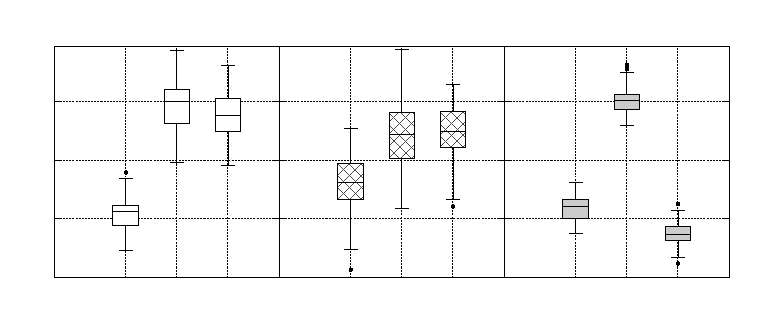
\includegraphics[width={360.00bp},height={144.00bp}]{Fat_path}}%
    \gplfronttext
  \end{picture}%
\endgroup
}}
    \caption{fat-tree}
    \label{fig:time:fat}
  \end{subfigure}
   \begin{subfigure}[b]{0.79\linewidth}
    \resizebox{\textwidth}{!}{\footnotesize{% GNUPLOT: LaTeX picture with Postscript
\begingroup
  \fontfamily{Times-Roman}%
  \selectfont
  \makeatletter
  \providecommand\color[2][]{%
    \GenericError{(gnuplot) \space\space\space\@spaces}{%
      Package color not loaded in conjunction with
      terminal option `colourtext'%
    }{See the gnuplot documentation for explanation.%
    }{Either use 'blacktext' in gnuplot or load the package
      color.sty in LaTeX.}%
    \renewcommand\color[2][]{}%
  }%
  \providecommand\includegraphics[2][]{%
    \GenericError{(gnuplot) \space\space\space\@spaces}{%
      Package graphicx or graphics not loaded%
    }{See the gnuplot documentation for explanation.%
    }{The gnuplot epslatex terminal needs graphicx.sty or graphics.sty.}%
    \renewcommand\includegraphics[2][]{}%
  }%
  \providecommand\rotatebox[2]{#2}%
  \@ifundefined{ifGPcolor}{%
    \newif\ifGPcolor
    \GPcolortrue
  }{}%
  \@ifundefined{ifGPblacktext}{%
    \newif\ifGPblacktext
    \GPblacktexttrue
  }{}%
  % define a \g@addto@macro without @ in the name:
  \let\gplgaddtomacro\g@addto@macro
  % define empty templates for all commands taking text:
  \gdef\gplbacktext{}%
  \gdef\gplfronttext{}%
  \makeatother
  \ifGPblacktext
    % no textcolor at all
    \def\colorrgb#1{}%
    \def\colorgray#1{}%
  \else
    % gray or color?
    \ifGPcolor
      \def\colorrgb#1{\color[rgb]{#1}}%
      \def\colorgray#1{\color[gray]{#1}}%
      \expandafter\def\csname LTw\endcsname{\color{white}}%
      \expandafter\def\csname LTb\endcsname{\color{black}}%
      \expandafter\def\csname LTa\endcsname{\color{black}}%
      \expandafter\def\csname LT0\endcsname{\color[rgb]{1,0,0}}%
      \expandafter\def\csname LT1\endcsname{\color[rgb]{0,1,0}}%
      \expandafter\def\csname LT2\endcsname{\color[rgb]{0,0,1}}%
      \expandafter\def\csname LT3\endcsname{\color[rgb]{1,0,1}}%
      \expandafter\def\csname LT4\endcsname{\color[rgb]{0,1,1}}%
      \expandafter\def\csname LT5\endcsname{\color[rgb]{1,1,0}}%
      \expandafter\def\csname LT6\endcsname{\color[rgb]{0,0,0}}%
      \expandafter\def\csname LT7\endcsname{\color[rgb]{1,0.3,0}}%
      \expandafter\def\csname LT8\endcsname{\color[rgb]{0.5,0.5,0.5}}%
    \else
      % gray
      \def\colorrgb#1{\color{black}}%
      \def\colorgray#1{\color[gray]{#1}}%
      \expandafter\def\csname LTw\endcsname{\color{white}}%
      \expandafter\def\csname LTb\endcsname{\color{black}}%
      \expandafter\def\csname LTa\endcsname{\color{black}}%
      \expandafter\def\csname LT0\endcsname{\color{black}}%
      \expandafter\def\csname LT1\endcsname{\color{black}}%
      \expandafter\def\csname LT2\endcsname{\color{black}}%
      \expandafter\def\csname LT3\endcsname{\color{black}}%
      \expandafter\def\csname LT4\endcsname{\color{black}}%
      \expandafter\def\csname LT5\endcsname{\color{black}}%
      \expandafter\def\csname LT6\endcsname{\color{black}}%
      \expandafter\def\csname LT7\endcsname{\color{black}}%
      \expandafter\def\csname LT8\endcsname{\color{black}}%
    \fi
  \fi
    \setlength{\unitlength}{0.0500bp}%
    \ifx\gptboxheight\undefined%
      \newlength{\gptboxheight}%
      \newlength{\gptboxwidth}%
      \newsavebox{\gptboxtext}%
    \fi%
    \setlength{\fboxrule}{0.5pt}%
    \setlength{\fboxsep}{1pt}%
\begin{picture}(7200.00,2880.00)%
    \gplgaddtomacro\gplbacktext{%
      \csname LTb\endcsname%%
      \put(782,528){\makebox(0,0)[r]{\strut{}$1900$}}%
      \csname LTb\endcsname%%
      \put(782,1089){\makebox(0,0)[r]{\strut{}$2100$}}%
      \csname LTb\endcsname%%
      \put(782,1651){\makebox(0,0)[r]{\strut{}$2300$}}%
      \csname LTb\endcsname%%
      \put(782,2212){\makebox(0,0)[r]{\strut{}$2500$}}%
      \csname LTb\endcsname%%
      \put(1126,242){\rotatebox{25}{\makebox(0,0)[r]{\strut{}SCC}}}%
      \csname LTb\endcsname%%
      \put(1617,242){\rotatebox{25}{\makebox(0,0)[r]{\strut{}CU}}}%
      \csname LTb\endcsname%%
      \put(2107,242){\rotatebox{25}{\makebox(0,0)[r]{\strut{}RWC}}}%
    }%
    \gplgaddtomacro\gplfronttext{%
      \csname LTb\endcsname%%
      \put(126,1482){\rotatebox{-270}{\makebox(0,0){\strut{}Time (ms)}}}%
      \put(1439,2701){\makebox(0,0){\strut{}Nimble}}%
    }%
    \gplgaddtomacro\gplbacktext{%
      \csname LTb\endcsname%%
      \put(2942,528){\makebox(0,0)[r]{\strut{}$2600$}}%
      \csname LTb\endcsname%%
      \put(2942,1089){\makebox(0,0)[r]{\strut{}$3000$}}%
      \csname LTb\endcsname%%
      \put(2942,1651){\makebox(0,0)[r]{\strut{}$3400$}}%
      \csname LTb\endcsname%%
      \put(2942,2212){\makebox(0,0)[r]{\strut{}$3800$}}%
      \csname LTb\endcsname%%
      \put(3286,242){\rotatebox{25}{\makebox(0,0)[r]{\strut{}SCC}}}%
      \csname LTb\endcsname%%
      \put(3777,242){\rotatebox{25}{\makebox(0,0)[r]{\strut{}CU}}}%
      \csname LTb\endcsname%%
      \put(4267,242){\rotatebox{25}{\makebox(0,0)[r]{\strut{}RWC}}}%
    }%
    \gplgaddtomacro\gplfronttext{%
      \csname LTb\endcsname%%
      \put(3599,2701){\makebox(0,0){\strut{}SwingState}}%
    }%
    \gplgaddtomacro\gplbacktext{%
      \csname LTb\endcsname%%
      \put(5102,528){\makebox(0,0)[r]{\strut{}$6600$}}%
      \csname LTb\endcsname%%
      \put(5102,1089){\makebox(0,0)[r]{\strut{}$7600$}}%
      \csname LTb\endcsname%%
      \put(5102,1651){\makebox(0,0)[r]{\strut{}$8600$}}%
      \csname LTb\endcsname%%
      \put(5102,2212){\makebox(0,0)[r]{\strut{}$9600$}}%
      \csname LTb\endcsname%%
      \put(5446,242){\rotatebox{25}{\makebox(0,0)[r]{\strut{}SCC}}}%
      \csname LTb\endcsname%%
      \put(5937,242){\rotatebox{25}{\makebox(0,0)[r]{\strut{}CU}}}%
      \csname LTb\endcsname%%
      \put(6427,242){\rotatebox{25}{\makebox(0,0)[r]{\strut{}RWC}}}%
    }%
    \gplgaddtomacro\gplfronttext{%
      \csname LTb\endcsname%%
      \put(5759,2701){\makebox(0,0){\strut{}OpenNF}}%
    }%
    \gplbacktext
    \put(0,0){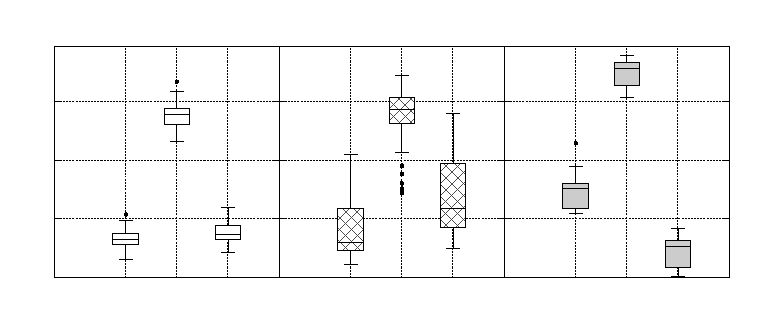
\includegraphics{Forthnet_path}}%
    \gplfronttext
  \end{picture}%
\endgroup
}}
    \caption{Forthnet}
    \label{fig:time:forthnet}
  \end{subfigure}
\caption{NF migration and path change times}
\label{fig:time}
\end{figure}



\iffalse
\begin{figure}[h!]
\centering
\begin{minipage}{0.49\linewidth}
   \begin{subfigure}[b]{0.99\linewidth}
    \resizebox{\textwidth}{!}{\footnotesize{% GNUPLOT: LaTeX picture with Postscript
\begingroup
  \fontfamily{Times-Roman}%
  \selectfont
  \makeatletter
  \providecommand\color[2][]{%
    \GenericError{(gnuplot) \space\space\space\@spaces}{%
      Package color not loaded in conjunction with
      terminal option `colourtext'%
    }{See the gnuplot documentation for explanation.%
    }{Either use 'blacktext' in gnuplot or load the package
      color.sty in LaTeX.}%
    \renewcommand\color[2][]{}%
  }%
  \providecommand\includegraphics[2][]{%
    \GenericError{(gnuplot) \space\space\space\@spaces}{%
      Package graphicx or graphics not loaded%
    }{See the gnuplot documentation for explanation.%
    }{The gnuplot epslatex terminal needs graphicx.sty or graphics.sty.}%
    \renewcommand\includegraphics[2][]{}%
  }%
  \providecommand\rotatebox[2]{#2}%
  \@ifundefined{ifGPcolor}{%
    \newif\ifGPcolor
    \GPcolortrue
  }{}%
  \@ifundefined{ifGPblacktext}{%
    \newif\ifGPblacktext
    \GPblacktexttrue
  }{}%
  % define a \g@addto@macro without @ in the name:
  \let\gplgaddtomacro\g@addto@macro
  % define empty templates for all commands taking text:
  \gdef\gplbacktext{}%
  \gdef\gplfronttext{}%
  \makeatother
  \ifGPblacktext
    % no textcolor at all
    \def\colorrgb#1{}%
    \def\colorgray#1{}%
  \else
    % gray or color?
    \ifGPcolor
      \def\colorrgb#1{\color[rgb]{#1}}%
      \def\colorgray#1{\color[gray]{#1}}%
      \expandafter\def\csname LTw\endcsname{\color{white}}%
      \expandafter\def\csname LTb\endcsname{\color{black}}%
      \expandafter\def\csname LTa\endcsname{\color{black}}%
      \expandafter\def\csname LT0\endcsname{\color[rgb]{1,0,0}}%
      \expandafter\def\csname LT1\endcsname{\color[rgb]{0,1,0}}%
      \expandafter\def\csname LT2\endcsname{\color[rgb]{0,0,1}}%
      \expandafter\def\csname LT3\endcsname{\color[rgb]{1,0,1}}%
      \expandafter\def\csname LT4\endcsname{\color[rgb]{0,1,1}}%
      \expandafter\def\csname LT5\endcsname{\color[rgb]{1,1,0}}%
      \expandafter\def\csname LT6\endcsname{\color[rgb]{0,0,0}}%
      \expandafter\def\csname LT7\endcsname{\color[rgb]{1,0.3,0}}%
      \expandafter\def\csname LT8\endcsname{\color[rgb]{0.5,0.5,0.5}}%
    \else
      % gray
      \def\colorrgb#1{\color{black}}%
      \def\colorgray#1{\color[gray]{#1}}%
      \expandafter\def\csname LTw\endcsname{\color{white}}%
      \expandafter\def\csname LTb\endcsname{\color{black}}%
      \expandafter\def\csname LTa\endcsname{\color{black}}%
      \expandafter\def\csname LT0\endcsname{\color{black}}%
      \expandafter\def\csname LT1\endcsname{\color{black}}%
      \expandafter\def\csname LT2\endcsname{\color{black}}%
      \expandafter\def\csname LT3\endcsname{\color{black}}%
      \expandafter\def\csname LT4\endcsname{\color{black}}%
      \expandafter\def\csname LT5\endcsname{\color{black}}%
      \expandafter\def\csname LT6\endcsname{\color{black}}%
      \expandafter\def\csname LT7\endcsname{\color{black}}%
      \expandafter\def\csname LT8\endcsname{\color{black}}%
    \fi
  \fi
    \setlength{\unitlength}{0.0500bp}%
    \ifx\gptboxheight\undefined%
      \newlength{\gptboxheight}%
      \newlength{\gptboxwidth}%
      \newsavebox{\gptboxtext}%
    \fi%
    \setlength{\fboxrule}{0.5pt}%
    \setlength{\fboxsep}{1pt}%
\begin{picture}(5760.00,2880.00)%
    \gplgaddtomacro\gplbacktext{%
      \csname LTb\endcsname%%
      \put(686,554){\makebox(0,0)[r]{\strut{}$12250$}}%
      \put(686,1043){\makebox(0,0)[r]{\strut{}$12500$}}%
      \put(686,1532){\makebox(0,0)[r]{\strut{}$12750$}}%
      \put(686,2021){\makebox(0,0)[r]{\strut{}$13000$}}%
      \put(686,2510){\makebox(0,0)[r]{\strut{}$13250$}}%
      \put(770,252){\makebox(0,0){\strut{}$0$}}%
      \put(1260,252){\makebox(0,0){\strut{}$500$}}%
      \put(1750,252){\makebox(0,0){\strut{}$1000$}}%
      \put(2240,252){\makebox(0,0){\strut{}$1500$}}%
      \put(2730,252){\makebox(0,0){\strut{}$2000$}}%
      \put(3220,252){\makebox(0,0){\strut{}$2500$}}%
      \put(3710,252){\makebox(0,0){\strut{}$3000$}}%
      \put(4200,252){\makebox(0,0){\strut{}$3500$}}%
      \put(4690,252){\makebox(0,0){\strut{}$4000$}}%
      \put(5180,252){\makebox(0,0){\strut{}$4500$}}%
    }%
    \gplgaddtomacro\gplfronttext{%
      \csname LTb\endcsname%%
      \put(168,1474){\rotatebox{-270}{\makebox(0,0){\strut{}Total number of rules}}}%
      \put(3138,98){\makebox(0,0){\strut{}Time (ms)}}%
      \csname LTb\endcsname%%
      \put(1133,2733){\makebox(0,0)[l]{\strut{}SCC+Nimble}}%
      \csname LTb\endcsname%%
      \put(2792,2733){\makebox(0,0)[l]{\strut{}SCC+OpenNF}}%
      \csname LTb\endcsname%%
      \put(4451,2733){\makebox(0,0)[l]{\strut{}SCC+SwingState}}%
    }%
    \gplbacktext
    \put(0,0){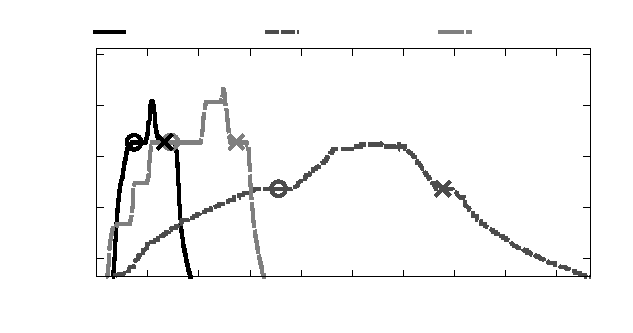
\includegraphics{SCCRuleFat}}%
    \gplfronttext
  \end{picture}%
\endgroup
}}
    \caption{SCC}
    \label{fig:rule_number:fat:scc}
  \end{subfigure}
  \par\bigskip
  \begin{subfigure}[b]{0.99\linewidth}
    \resizebox{\textwidth}{!}{\footnotesize{% GNUPLOT: LaTeX picture with Postscript
\begingroup
  \fontfamily{Times-Roman}%
  \selectfont
  \makeatletter
  \providecommand\color[2][]{%
    \GenericError{(gnuplot) \space\space\space\@spaces}{%
      Package color not loaded in conjunction with
      terminal option `colourtext'%
    }{See the gnuplot documentation for explanation.%
    }{Either use 'blacktext' in gnuplot or load the package
      color.sty in LaTeX.}%
    \renewcommand\color[2][]{}%
  }%
  \providecommand\includegraphics[2][]{%
    \GenericError{(gnuplot) \space\space\space\@spaces}{%
      Package graphicx or graphics not loaded%
    }{See the gnuplot documentation for explanation.%
    }{The gnuplot epslatex terminal needs graphicx.sty or graphics.sty.}%
    \renewcommand\includegraphics[2][]{}%
  }%
  \providecommand\rotatebox[2]{#2}%
  \@ifundefined{ifGPcolor}{%
    \newif\ifGPcolor
    \GPcolortrue
  }{}%
  \@ifundefined{ifGPblacktext}{%
    \newif\ifGPblacktext
    \GPblacktexttrue
  }{}%
  % define a \g@addto@macro without @ in the name:
  \let\gplgaddtomacro\g@addto@macro
  % define empty templates for all commands taking text:
  \gdef\gplbacktext{}%
  \gdef\gplfronttext{}%
  \makeatother
  \ifGPblacktext
    % no textcolor at all
    \def\colorrgb#1{}%
    \def\colorgray#1{}%
  \else
    % gray or color?
    \ifGPcolor
      \def\colorrgb#1{\color[rgb]{#1}}%
      \def\colorgray#1{\color[gray]{#1}}%
      \expandafter\def\csname LTw\endcsname{\color{white}}%
      \expandafter\def\csname LTb\endcsname{\color{black}}%
      \expandafter\def\csname LTa\endcsname{\color{black}}%
      \expandafter\def\csname LT0\endcsname{\color[rgb]{1,0,0}}%
      \expandafter\def\csname LT1\endcsname{\color[rgb]{0,1,0}}%
      \expandafter\def\csname LT2\endcsname{\color[rgb]{0,0,1}}%
      \expandafter\def\csname LT3\endcsname{\color[rgb]{1,0,1}}%
      \expandafter\def\csname LT4\endcsname{\color[rgb]{0,1,1}}%
      \expandafter\def\csname LT5\endcsname{\color[rgb]{1,1,0}}%
      \expandafter\def\csname LT6\endcsname{\color[rgb]{0,0,0}}%
      \expandafter\def\csname LT7\endcsname{\color[rgb]{1,0.3,0}}%
      \expandafter\def\csname LT8\endcsname{\color[rgb]{0.5,0.5,0.5}}%
    \else
      % gray
      \def\colorrgb#1{\color{black}}%
      \def\colorgray#1{\color[gray]{#1}}%
      \expandafter\def\csname LTw\endcsname{\color{white}}%
      \expandafter\def\csname LTb\endcsname{\color{black}}%
      \expandafter\def\csname LTa\endcsname{\color{black}}%
      \expandafter\def\csname LT0\endcsname{\color{black}}%
      \expandafter\def\csname LT1\endcsname{\color{black}}%
      \expandafter\def\csname LT2\endcsname{\color{black}}%
      \expandafter\def\csname LT3\endcsname{\color{black}}%
      \expandafter\def\csname LT4\endcsname{\color{black}}%
      \expandafter\def\csname LT5\endcsname{\color{black}}%
      \expandafter\def\csname LT6\endcsname{\color{black}}%
      \expandafter\def\csname LT7\endcsname{\color{black}}%
      \expandafter\def\csname LT8\endcsname{\color{black}}%
    \fi
  \fi
    \setlength{\unitlength}{0.0500bp}%
    \ifx\gptboxheight\undefined%
      \newlength{\gptboxheight}%
      \newlength{\gptboxwidth}%
      \newsavebox{\gptboxtext}%
    \fi%
    \setlength{\fboxrule}{0.5pt}%
    \setlength{\fboxsep}{1pt}%
\begin{picture}(5760.00,2880.00)%
    \gplgaddtomacro\gplbacktext{%
      \csname LTb\endcsname%%
      \put(686,588){\makebox(0,0)[r]{\strut{}$12300$}}%
      \put(686,1039){\makebox(0,0)[r]{\strut{}$12600$}}%
      \put(686,1490){\makebox(0,0)[r]{\strut{}$12900$}}%
      \put(686,1940){\makebox(0,0)[r]{\strut{}$13200$}}%
      \put(686,2391){\makebox(0,0)[r]{\strut{}$13500$}}%
      \put(770,252){\makebox(0,0){\strut{}$0$}}%
      \put(1557,252){\makebox(0,0){\strut{}$1000$}}%
      \put(2344,252){\makebox(0,0){\strut{}$2000$}}%
      \put(3130,252){\makebox(0,0){\strut{}$3000$}}%
      \put(3917,252){\makebox(0,0){\strut{}$4000$}}%
      \put(4704,252){\makebox(0,0){\strut{}$5000$}}%
      \put(5491,252){\makebox(0,0){\strut{}$6000$}}%
    }%
    \gplgaddtomacro\gplfronttext{%
      \csname LTb\endcsname%%
      \put(168,1474){\rotatebox{-270}{\makebox(0,0){\strut{}Total number of rules}}}%
      \put(3138,98){\makebox(0,0){\strut{}Time (ms)}}%
      \csname LTb\endcsname%%
      \put(1259,2733){\makebox(0,0)[l]{\strut{}CU+Nimble}}%
      \csname LTb\endcsname%%
      \put(2834,2733){\makebox(0,0)[l]{\strut{}CU+OpenNF}}%
      \csname LTb\endcsname%%
      \put(4409,2733){\makebox(0,0)[l]{\strut{}CU+SwingState}}%
    }%
    \gplbacktext
    \put(0,0){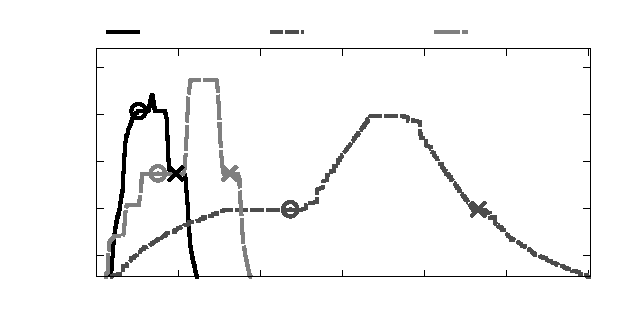
\includegraphics{CURuleFat}}%
    \gplfronttext
  \end{picture}%
\endgroup
}}
    \caption{CU}
    \label{fig:rule_number:fat:scc}
  \end{subfigure}
  \par\bigskip
  \begin{subfigure}[b]{0.99\linewidth}
    \resizebox{\textwidth}{!}{\footnotesize{% GNUPLOT: LaTeX picture with Postscript
\begingroup
  \fontfamily{Times-Roman}%
  \selectfont
  \makeatletter
  \providecommand\color[2][]{%
    \GenericError{(gnuplot) \space\space\space\@spaces}{%
      Package color not loaded in conjunction with
      terminal option `colourtext'%
    }{See the gnuplot documentation for explanation.%
    }{Either use 'blacktext' in gnuplot or load the package
      color.sty in LaTeX.}%
    \renewcommand\color[2][]{}%
  }%
  \providecommand\includegraphics[2][]{%
    \GenericError{(gnuplot) \space\space\space\@spaces}{%
      Package graphicx or graphics not loaded%
    }{See the gnuplot documentation for explanation.%
    }{The gnuplot epslatex terminal needs graphicx.sty or graphics.sty.}%
    \renewcommand\includegraphics[2][]{}%
  }%
  \providecommand\rotatebox[2]{#2}%
  \@ifundefined{ifGPcolor}{%
    \newif\ifGPcolor
    \GPcolortrue
  }{}%
  \@ifundefined{ifGPblacktext}{%
    \newif\ifGPblacktext
    \GPblacktexttrue
  }{}%
  % define a \g@addto@macro without @ in the name:
  \let\gplgaddtomacro\g@addto@macro
  % define empty templates for all commands taking text:
  \gdef\gplbacktext{}%
  \gdef\gplfronttext{}%
  \makeatother
  \ifGPblacktext
    % no textcolor at all
    \def\colorrgb#1{}%
    \def\colorgray#1{}%
  \else
    % gray or color?
    \ifGPcolor
      \def\colorrgb#1{\color[rgb]{#1}}%
      \def\colorgray#1{\color[gray]{#1}}%
      \expandafter\def\csname LTw\endcsname{\color{white}}%
      \expandafter\def\csname LTb\endcsname{\color{black}}%
      \expandafter\def\csname LTa\endcsname{\color{black}}%
      \expandafter\def\csname LT0\endcsname{\color[rgb]{1,0,0}}%
      \expandafter\def\csname LT1\endcsname{\color[rgb]{0,1,0}}%
      \expandafter\def\csname LT2\endcsname{\color[rgb]{0,0,1}}%
      \expandafter\def\csname LT3\endcsname{\color[rgb]{1,0,1}}%
      \expandafter\def\csname LT4\endcsname{\color[rgb]{0,1,1}}%
      \expandafter\def\csname LT5\endcsname{\color[rgb]{1,1,0}}%
      \expandafter\def\csname LT6\endcsname{\color[rgb]{0,0,0}}%
      \expandafter\def\csname LT7\endcsname{\color[rgb]{1,0.3,0}}%
      \expandafter\def\csname LT8\endcsname{\color[rgb]{0.5,0.5,0.5}}%
    \else
      % gray
      \def\colorrgb#1{\color{black}}%
      \def\colorgray#1{\color[gray]{#1}}%
      \expandafter\def\csname LTw\endcsname{\color{white}}%
      \expandafter\def\csname LTb\endcsname{\color{black}}%
      \expandafter\def\csname LTa\endcsname{\color{black}}%
      \expandafter\def\csname LT0\endcsname{\color{black}}%
      \expandafter\def\csname LT1\endcsname{\color{black}}%
      \expandafter\def\csname LT2\endcsname{\color{black}}%
      \expandafter\def\csname LT3\endcsname{\color{black}}%
      \expandafter\def\csname LT4\endcsname{\color{black}}%
      \expandafter\def\csname LT5\endcsname{\color{black}}%
      \expandafter\def\csname LT6\endcsname{\color{black}}%
      \expandafter\def\csname LT7\endcsname{\color{black}}%
      \expandafter\def\csname LT8\endcsname{\color{black}}%
    \fi
  \fi
    \setlength{\unitlength}{0.0500bp}%
    \ifx\gptboxheight\undefined%
      \newlength{\gptboxheight}%
      \newlength{\gptboxwidth}%
      \newsavebox{\gptboxtext}%
    \fi%
    \setlength{\fboxrule}{0.5pt}%
    \setlength{\fboxsep}{1pt}%
\begin{picture}(5760.00,2880.00)%
    \gplgaddtomacro\gplbacktext{%
      \csname LTb\endcsname%%
      \put(686,547){\makebox(0,0)[r]{\strut{}$12250$}}%
      \put(686,1015){\makebox(0,0)[r]{\strut{}$12500$}}%
      \put(686,1484){\makebox(0,0)[r]{\strut{}$12750$}}%
      \put(686,1952){\makebox(0,0)[r]{\strut{}$13000$}}%
      \put(686,2421){\makebox(0,0)[r]{\strut{}$13250$}}%
      \put(770,252){\makebox(0,0){\strut{}$0$}}%
      \put(1272,252){\makebox(0,0){\strut{}$500$}}%
      \put(1775,252){\makebox(0,0){\strut{}$1000$}}%
      \put(2277,252){\makebox(0,0){\strut{}$1500$}}%
      \put(2780,252){\makebox(0,0){\strut{}$2000$}}%
      \put(3282,252){\makebox(0,0){\strut{}$2500$}}%
      \put(3785,252){\makebox(0,0){\strut{}$3000$}}%
      \put(4287,252){\makebox(0,0){\strut{}$3500$}}%
      \put(4790,252){\makebox(0,0){\strut{}$4000$}}%
      \put(5292,252){\makebox(0,0){\strut{}$4500$}}%
    }%
    \gplgaddtomacro\gplfronttext{%
      \csname LTb\endcsname%%
      \put(168,1474){\rotatebox{-270}{\makebox(0,0){\strut{}Total number of rules}}}%
      \put(3138,98){\makebox(0,0){\strut{}Time (ms)}}%
      \csname LTb\endcsname%%
      \put(1133,2733){\makebox(0,0)[l]{\strut{}RWC+Nimble}}%
      \csname LTb\endcsname%%
      \put(2792,2733){\makebox(0,0)[l]{\strut{}RWC+OpenNF}}%
      \csname LTb\endcsname%%
      \put(4451,2733){\makebox(0,0)[l]{\strut{}RWC+SwingState}}%
    }%
    \gplbacktext
    \put(0,0){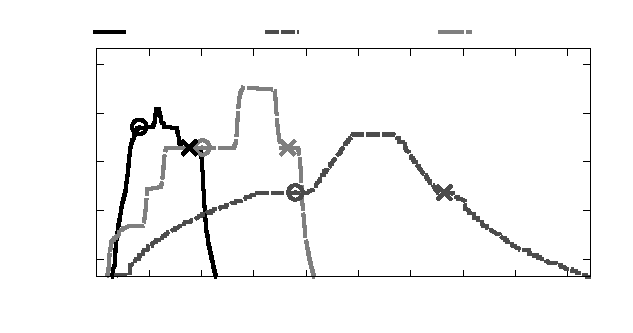
\includegraphics{RWCRuleFat}}%
    \gplfronttext
  \end{picture}%
\endgroup
}}
    \caption{\ourRouteUpdateName}
    \label{fig:rule_number:fat:cu}
  \end{subfigure}
  \caption{Rules in the network during 100 path changes and
    accompanying NF migrations for fat-tree topology; markers show
    completion of path changes ($\times$) and NF migrations
    ({\LARGE $\circ$})}
\label{fig:rule_number:fat}
\end{minipage}
\centering
\begin{minipage}{0.49\linewidth}
   \begin{subfigure}[b]{0.99\linewidth}
    \resizebox{\textwidth}{!}{\footnotesize{% GNUPLOT: LaTeX picture with Postscript
\begingroup
  \fontfamily{Times-Roman}%
  \selectfont
  \makeatletter
  \providecommand\color[2][]{%
    \GenericError{(gnuplot) \space\space\space\@spaces}{%
      Package color not loaded in conjunction with
      terminal option `colourtext'%
    }{See the gnuplot documentation for explanation.%
    }{Either use 'blacktext' in gnuplot or load the package
      color.sty in LaTeX.}%
    \renewcommand\color[2][]{}%
  }%
  \providecommand\includegraphics[2][]{%
    \GenericError{(gnuplot) \space\space\space\@spaces}{%
      Package graphicx or graphics not loaded%
    }{See the gnuplot documentation for explanation.%
    }{The gnuplot epslatex terminal needs graphicx.sty or graphics.sty.}%
    \renewcommand\includegraphics[2][]{}%
  }%
  \providecommand\rotatebox[2]{#2}%
  \@ifundefined{ifGPcolor}{%
    \newif\ifGPcolor
    \GPcolortrue
  }{}%
  \@ifundefined{ifGPblacktext}{%
    \newif\ifGPblacktext
    \GPblacktexttrue
  }{}%
  % define a \g@addto@macro without @ in the name:
  \let\gplgaddtomacro\g@addto@macro
  % define empty templates for all commands taking text:
  \gdef\gplbacktext{}%
  \gdef\gplfronttext{}%
  \makeatother
  \ifGPblacktext
    % no textcolor at all
    \def\colorrgb#1{}%
    \def\colorgray#1{}%
  \else
    % gray or color?
    \ifGPcolor
      \def\colorrgb#1{\color[rgb]{#1}}%
      \def\colorgray#1{\color[gray]{#1}}%
      \expandafter\def\csname LTw\endcsname{\color{white}}%
      \expandafter\def\csname LTb\endcsname{\color{black}}%
      \expandafter\def\csname LTa\endcsname{\color{black}}%
      \expandafter\def\csname LT0\endcsname{\color[rgb]{1,0,0}}%
      \expandafter\def\csname LT1\endcsname{\color[rgb]{0,1,0}}%
      \expandafter\def\csname LT2\endcsname{\color[rgb]{0,0,1}}%
      \expandafter\def\csname LT3\endcsname{\color[rgb]{1,0,1}}%
      \expandafter\def\csname LT4\endcsname{\color[rgb]{0,1,1}}%
      \expandafter\def\csname LT5\endcsname{\color[rgb]{1,1,0}}%
      \expandafter\def\csname LT6\endcsname{\color[rgb]{0,0,0}}%
      \expandafter\def\csname LT7\endcsname{\color[rgb]{1,0.3,0}}%
      \expandafter\def\csname LT8\endcsname{\color[rgb]{0.5,0.5,0.5}}%
    \else
      % gray
      \def\colorrgb#1{\color{black}}%
      \def\colorgray#1{\color[gray]{#1}}%
      \expandafter\def\csname LTw\endcsname{\color{white}}%
      \expandafter\def\csname LTb\endcsname{\color{black}}%
      \expandafter\def\csname LTa\endcsname{\color{black}}%
      \expandafter\def\csname LT0\endcsname{\color{black}}%
      \expandafter\def\csname LT1\endcsname{\color{black}}%
      \expandafter\def\csname LT2\endcsname{\color{black}}%
      \expandafter\def\csname LT3\endcsname{\color{black}}%
      \expandafter\def\csname LT4\endcsname{\color{black}}%
      \expandafter\def\csname LT5\endcsname{\color{black}}%
      \expandafter\def\csname LT6\endcsname{\color{black}}%
      \expandafter\def\csname LT7\endcsname{\color{black}}%
      \expandafter\def\csname LT8\endcsname{\color{black}}%
    \fi
  \fi
    \setlength{\unitlength}{0.0500bp}%
    \ifx\gptboxheight\undefined%
      \newlength{\gptboxheight}%
      \newlength{\gptboxwidth}%
      \newsavebox{\gptboxtext}%
    \fi%
    \setlength{\fboxrule}{0.5pt}%
    \setlength{\fboxsep}{1pt}%
\begin{picture}(5760.00,2880.00)%
    \gplgaddtomacro\gplbacktext{%
      \csname LTb\endcsname%%
      \put(686,553){\makebox(0,0)[r]{\strut{}$12000$}}%
      \put(686,1005){\makebox(0,0)[r]{\strut{}$12400$}}%
      \put(686,1456){\makebox(0,0)[r]{\strut{}$12800$}}%
      \put(686,1908){\makebox(0,0)[r]{\strut{}$13200$}}%
      \put(686,2360){\makebox(0,0)[r]{\strut{}$13600$}}%
      \put(770,252){\makebox(0,0){\strut{}$0$}}%
      \put(1627,252){\makebox(0,0){\strut{}$2000$}}%
      \put(2483,252){\makebox(0,0){\strut{}$4000$}}%
      \put(3340,252){\makebox(0,0){\strut{}$6000$}}%
      \put(4197,252){\makebox(0,0){\strut{}$8000$}}%
      \put(5053,252){\makebox(0,0){\strut{}$10000$}}%
    }%
    \gplgaddtomacro\gplfronttext{%
      \csname LTb\endcsname%%
      \put(168,1474){\rotatebox{-270}{\makebox(0,0){\strut{}Total number of rules}}}%
      \put(3138,98){\makebox(0,0){\strut{}Time (ms)}}%
      \csname LTb\endcsname%%
      \put(1133,2733){\makebox(0,0)[l]{\strut{}SCC+Nimble}}%
      \csname LTb\endcsname%%
      \put(2792,2733){\makebox(0,0)[l]{\strut{}SCC+OpenNF}}%
      \csname LTb\endcsname%%
      \put(4451,2733){\makebox(0,0)[l]{\strut{}SCC+SwingState}}%
    }%
    \gplbacktext
    \put(0,0){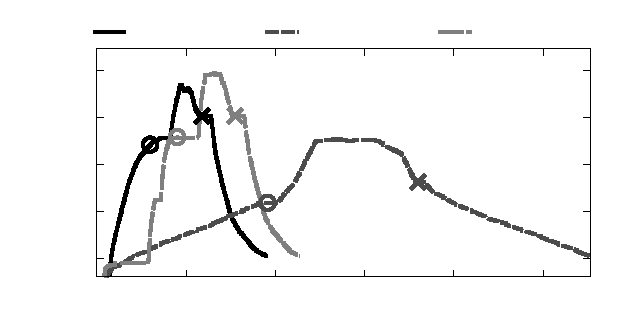
\includegraphics{SCCRuleForthnet}}%
    \gplfronttext
  \end{picture}%
\endgroup
}}
    \caption{SCC}
    \label{fig:rule_number:Forthnet:scc}
  \end{subfigure}
  \par\bigskip
  \begin{subfigure}[b]{0.99\linewidth}
    \resizebox{\textwidth}{!}{\footnotesize{% GNUPLOT: LaTeX picture with Postscript
\begingroup
  \fontfamily{Times-Roman}%
  \selectfont
  \makeatletter
  \providecommand\color[2][]{%
    \GenericError{(gnuplot) \space\space\space\@spaces}{%
      Package color not loaded in conjunction with
      terminal option `colourtext'%
    }{See the gnuplot documentation for explanation.%
    }{Either use 'blacktext' in gnuplot or load the package
      color.sty in LaTeX.}%
    \renewcommand\color[2][]{}%
  }%
  \providecommand\includegraphics[2][]{%
    \GenericError{(gnuplot) \space\space\space\@spaces}{%
      Package graphicx or graphics not loaded%
    }{See the gnuplot documentation for explanation.%
    }{The gnuplot epslatex terminal needs graphicx.sty or graphics.sty.}%
    \renewcommand\includegraphics[2][]{}%
  }%
  \providecommand\rotatebox[2]{#2}%
  \@ifundefined{ifGPcolor}{%
    \newif\ifGPcolor
    \GPcolortrue
  }{}%
  \@ifundefined{ifGPblacktext}{%
    \newif\ifGPblacktext
    \GPblacktexttrue
  }{}%
  % define a \g@addto@macro without @ in the name:
  \let\gplgaddtomacro\g@addto@macro
  % define empty templates for all commands taking text:
  \gdef\gplbacktext{}%
  \gdef\gplfronttext{}%
  \makeatother
  \ifGPblacktext
    % no textcolor at all
    \def\colorrgb#1{}%
    \def\colorgray#1{}%
  \else
    % gray or color?
    \ifGPcolor
      \def\colorrgb#1{\color[rgb]{#1}}%
      \def\colorgray#1{\color[gray]{#1}}%
      \expandafter\def\csname LTw\endcsname{\color{white}}%
      \expandafter\def\csname LTb\endcsname{\color{black}}%
      \expandafter\def\csname LTa\endcsname{\color{black}}%
      \expandafter\def\csname LT0\endcsname{\color[rgb]{1,0,0}}%
      \expandafter\def\csname LT1\endcsname{\color[rgb]{0,1,0}}%
      \expandafter\def\csname LT2\endcsname{\color[rgb]{0,0,1}}%
      \expandafter\def\csname LT3\endcsname{\color[rgb]{1,0,1}}%
      \expandafter\def\csname LT4\endcsname{\color[rgb]{0,1,1}}%
      \expandafter\def\csname LT5\endcsname{\color[rgb]{1,1,0}}%
      \expandafter\def\csname LT6\endcsname{\color[rgb]{0,0,0}}%
      \expandafter\def\csname LT7\endcsname{\color[rgb]{1,0.3,0}}%
      \expandafter\def\csname LT8\endcsname{\color[rgb]{0.5,0.5,0.5}}%
    \else
      % gray
      \def\colorrgb#1{\color{black}}%
      \def\colorgray#1{\color[gray]{#1}}%
      \expandafter\def\csname LTw\endcsname{\color{white}}%
      \expandafter\def\csname LTb\endcsname{\color{black}}%
      \expandafter\def\csname LTa\endcsname{\color{black}}%
      \expandafter\def\csname LT0\endcsname{\color{black}}%
      \expandafter\def\csname LT1\endcsname{\color{black}}%
      \expandafter\def\csname LT2\endcsname{\color{black}}%
      \expandafter\def\csname LT3\endcsname{\color{black}}%
      \expandafter\def\csname LT4\endcsname{\color{black}}%
      \expandafter\def\csname LT5\endcsname{\color{black}}%
      \expandafter\def\csname LT6\endcsname{\color{black}}%
      \expandafter\def\csname LT7\endcsname{\color{black}}%
      \expandafter\def\csname LT8\endcsname{\color{black}}%
    \fi
  \fi
    \setlength{\unitlength}{0.0500bp}%
    \ifx\gptboxheight\undefined%
      \newlength{\gptboxheight}%
      \newlength{\gptboxwidth}%
      \newsavebox{\gptboxtext}%
    \fi%
    \setlength{\fboxrule}{0.5pt}%
    \setlength{\fboxsep}{1pt}%
\begin{picture}(5760.00,2880.00)%
    \gplgaddtomacro\gplbacktext{%
      \csname LTb\endcsname%%
      \put(686,417){\makebox(0,0)[r]{\strut{}$11900$}}%
      \put(686,920){\makebox(0,0)[r]{\strut{}$12600$}}%
      \put(686,1422){\makebox(0,0)[r]{\strut{}$13300$}}%
      \put(686,1924){\makebox(0,0)[r]{\strut{}$14000$}}%
      \put(686,2427){\makebox(0,0)[r]{\strut{}$14700$}}%
      \put(770,252){\makebox(0,0){\strut{}$0$}}%
      \put(1509,252){\makebox(0,0){\strut{}$2000$}}%
      \put(2248,252){\makebox(0,0){\strut{}$4000$}}%
      \put(2986,252){\makebox(0,0){\strut{}$6000$}}%
      \put(3725,252){\makebox(0,0){\strut{}$8000$}}%
      \put(4464,252){\makebox(0,0){\strut{}$10000$}}%
      \put(5203,252){\makebox(0,0){\strut{}$12000$}}%
    }%
    \gplgaddtomacro\gplfronttext{%
      \csname LTb\endcsname%%
      \put(168,1474){\rotatebox{-270}{\makebox(0,0){\strut{}Total number of rules}}}%
      \put(3138,98){\makebox(0,0){\strut{}Time (ms)}}%
      \csname LTb\endcsname%%
      \put(1259,2733){\makebox(0,0)[l]{\strut{}CU+Nimble}}%
      \csname LTb\endcsname%%
      \put(2834,2733){\makebox(0,0)[l]{\strut{}CU+OpenNF}}%
      \csname LTb\endcsname%%
      \put(4409,2733){\makebox(0,0)[l]{\strut{}CU+SwingState}}%
    }%
    \gplbacktext
    \put(0,0){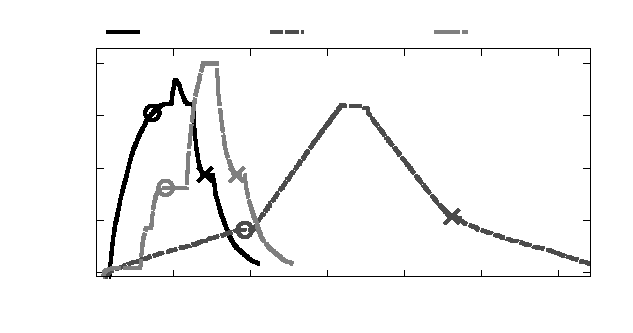
\includegraphics{CURuleForthnet}}%
    \gplfronttext
  \end{picture}%
\endgroup
}}
    \caption{CU}
    \label{fig:rule_number:Forthnet:scc}
  \end{subfigure}
  \par\bigskip
  \begin{subfigure}[b]{0.99\linewidth}
    \resizebox{\textwidth}{!}{\small{% GNUPLOT: LaTeX picture with Postscript
\begingroup
  \fontfamily{Times-Roman}%
  \selectfont
  \makeatletter
  \providecommand\color[2][]{%
    \GenericError{(gnuplot) \space\space\space\@spaces}{%
      Package color not loaded in conjunction with
      terminal option `colourtext'%
    }{See the gnuplot documentation for explanation.%
    }{Either use 'blacktext' in gnuplot or load the package
      color.sty in LaTeX.}%
    \renewcommand\color[2][]{}%
  }%
  \providecommand\includegraphics[2][]{%
    \GenericError{(gnuplot) \space\space\space\@spaces}{%
      Package graphicx or graphics not loaded%
    }{See the gnuplot documentation for explanation.%
    }{The gnuplot epslatex terminal needs graphicx.sty or graphics.sty.}%
    \renewcommand\includegraphics[2][]{}%
  }%
  \providecommand\rotatebox[2]{#2}%
  \@ifundefined{ifGPcolor}{%
    \newif\ifGPcolor
    \GPcolortrue
  }{}%
  \@ifundefined{ifGPblacktext}{%
    \newif\ifGPblacktext
    \GPblacktexttrue
  }{}%
  % define a \g@addto@macro without @ in the name:
  \let\gplgaddtomacro\g@addto@macro
  % define empty templates for all commands taking text:
  \gdef\gplbacktext{}%
  \gdef\gplfronttext{}%
  \makeatother
  \ifGPblacktext
    % no textcolor at all
    \def\colorrgb#1{}%
    \def\colorgray#1{}%
  \else
    % gray or color?
    \ifGPcolor
      \def\colorrgb#1{\color[rgb]{#1}}%
      \def\colorgray#1{\color[gray]{#1}}%
      \expandafter\def\csname LTw\endcsname{\color{white}}%
      \expandafter\def\csname LTb\endcsname{\color{black}}%
      \expandafter\def\csname LTa\endcsname{\color{black}}%
      \expandafter\def\csname LT0\endcsname{\color[rgb]{1,0,0}}%
      \expandafter\def\csname LT1\endcsname{\color[rgb]{0,1,0}}%
      \expandafter\def\csname LT2\endcsname{\color[rgb]{0,0,1}}%
      \expandafter\def\csname LT3\endcsname{\color[rgb]{1,0,1}}%
      \expandafter\def\csname LT4\endcsname{\color[rgb]{0,1,1}}%
      \expandafter\def\csname LT5\endcsname{\color[rgb]{1,1,0}}%
      \expandafter\def\csname LT6\endcsname{\color[rgb]{0,0,0}}%
      \expandafter\def\csname LT7\endcsname{\color[rgb]{1,0.3,0}}%
      \expandafter\def\csname LT8\endcsname{\color[rgb]{0.5,0.5,0.5}}%
    \else
      % gray
      \def\colorrgb#1{\color{black}}%
      \def\colorgray#1{\color[gray]{#1}}%
      \expandafter\def\csname LTw\endcsname{\color{white}}%
      \expandafter\def\csname LTb\endcsname{\color{black}}%
      \expandafter\def\csname LTa\endcsname{\color{black}}%
      \expandafter\def\csname LT0\endcsname{\color{black}}%
      \expandafter\def\csname LT1\endcsname{\color{black}}%
      \expandafter\def\csname LT2\endcsname{\color{black}}%
      \expandafter\def\csname LT3\endcsname{\color{black}}%
      \expandafter\def\csname LT4\endcsname{\color{black}}%
      \expandafter\def\csname LT5\endcsname{\color{black}}%
      \expandafter\def\csname LT6\endcsname{\color{black}}%
      \expandafter\def\csname LT7\endcsname{\color{black}}%
      \expandafter\def\csname LT8\endcsname{\color{black}}%
    \fi
  \fi
    \setlength{\unitlength}{0.0500bp}%
    \ifx\gptboxheight\undefined%
      \newlength{\gptboxheight}%
      \newlength{\gptboxwidth}%
      \newsavebox{\gptboxtext}%
    \fi%
    \setlength{\fboxrule}{0.5pt}%
    \setlength{\fboxsep}{1pt}%
\begin{picture}(5760.00,2880.00)%
    \gplgaddtomacro\gplbacktext{%
      \csname LTb\endcsname%%
      \put(686,540){\makebox(0,0)[r]{\strut{}$12000$}}%
      \put(686,1061){\makebox(0,0)[r]{\strut{}$12500$}}%
      \put(686,1582){\makebox(0,0)[r]{\strut{}$13000$}}%
      \put(686,2104){\makebox(0,0)[r]{\strut{}$13500$}}%
      \put(770,252){\makebox(0,0){\strut{}$0$}}%
      \put(1716,252){\makebox(0,0){\strut{}$2000$}}%
      \put(2662,252){\makebox(0,0){\strut{}$4000$}}%
      \put(3608,252){\makebox(0,0){\strut{}$6000$}}%
      \put(4554,252){\makebox(0,0){\strut{}$8000$}}%
      \put(5500,252){\makebox(0,0){\strut{}$10000$}}%
    }%
    \gplgaddtomacro\gplfronttext{%
      \csname LTb\endcsname%%
      \put(168,1474){\rotatebox{-270}{\makebox(0,0){\strut{}Total number of rules}}}%
      \put(3138,98){\makebox(0,0){\strut{}Time (ms)}}%
      \csname LTb\endcsname%%
      \put(1133,2733){\makebox(0,0)[l]{\strut{}RWC+Nimble}}%
      \csname LTb\endcsname%%
      \put(2792,2733){\makebox(0,0)[l]{\strut{}RWC+OpenNF}}%
      \csname LTb\endcsname%%
      \put(4451,2733){\makebox(0,0)[l]{\strut{}RWC+SwingState}}%
    }%
    \gplbacktext
    \put(0,0){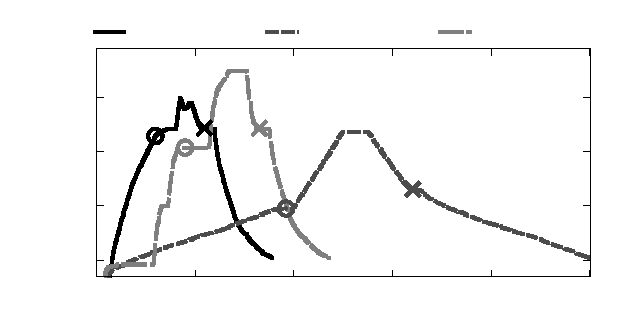
\includegraphics{RWCRuleForthnet}}%
    \gplfronttext
  \end{picture}%
\endgroup
}}
    \caption{\ourRouteUpdateName}
    \label{fig:rule_number:Forthnet:cu}
  \end{subfigure}
  \caption{Rules in the network during 178 path changes and
    accompanying NF migrations for Forthnet topology; markers show
    completion of path changes ($\times$) and NF migrations
    ({\LARGE $\circ$})}
\label{fig:rule_number:Forthnet}
\end{minipage}
\end{figure}
\fi

We measured the performance of our algorithm for NF migration and path
change, in comparison to other algorithms.  Each evaluation involved
$100$ runs, in which hosts sent $100$ packets per second for each
flow. \figref{fig:time} demonstrates the times required to finish both
NF migration and path changes; \figref{fig:time:fat} shows times for
100 path changes with two NF migrations per path change in a fat-tree
topology ($\portsPerSwitch = 8$), and \figref{fig:time:forthnet} shows
times for 178 path changes with three NF migrations per path change in
the Forthnet topology induced by breaking its ``busiest'' link
carrying the most flows.  Each boxplot in these figures represents 100
points, one per run; the box marks the first, second (median), and
third quartiles, and whiskers extend to cover points within
$1.5\times$ the interquartile range.  Outliers are shown as dots.


As can be seen in these figures, \sysname performed much faster than
SwingState and OpenNF, since NF migration and path change were
executed simultaneously. OpenNF required much more time to perform the
updates because it uses a single controller to buffer and redistribute
packets. Upon receiving a large number of incoming packets, the
controller consumed a lot of resources to process these packets, which
significantly slowed down the rule-update process.


\begin{figure}[H]
\centering
   \begin{subfigure}[b]{0.69\linewidth}
    \resizebox{\textwidth}{!}{\footnotesize{% GNUPLOT: LaTeX picture with Postscript
\begingroup
  \fontfamily{Times-Roman}%
  \selectfont
  \makeatletter
  \providecommand\color[2][]{%
    \GenericError{(gnuplot) \space\space\space\@spaces}{%
      Package color not loaded in conjunction with
      terminal option `colourtext'%
    }{See the gnuplot documentation for explanation.%
    }{Either use 'blacktext' in gnuplot or load the package
      color.sty in LaTeX.}%
    \renewcommand\color[2][]{}%
  }%
  \providecommand\includegraphics[2][]{%
    \GenericError{(gnuplot) \space\space\space\@spaces}{%
      Package graphicx or graphics not loaded%
    }{See the gnuplot documentation for explanation.%
    }{The gnuplot epslatex terminal needs graphicx.sty or graphics.sty.}%
    \renewcommand\includegraphics[2][]{}%
  }%
  \providecommand\rotatebox[2]{#2}%
  \@ifundefined{ifGPcolor}{%
    \newif\ifGPcolor
    \GPcolortrue
  }{}%
  \@ifundefined{ifGPblacktext}{%
    \newif\ifGPblacktext
    \GPblacktexttrue
  }{}%
  % define a \g@addto@macro without @ in the name:
  \let\gplgaddtomacro\g@addto@macro
  % define empty templates for all commands taking text:
  \gdef\gplbacktext{}%
  \gdef\gplfronttext{}%
  \makeatother
  \ifGPblacktext
    % no textcolor at all
    \def\colorrgb#1{}%
    \def\colorgray#1{}%
  \else
    % gray or color?
    \ifGPcolor
      \def\colorrgb#1{\color[rgb]{#1}}%
      \def\colorgray#1{\color[gray]{#1}}%
      \expandafter\def\csname LTw\endcsname{\color{white}}%
      \expandafter\def\csname LTb\endcsname{\color{black}}%
      \expandafter\def\csname LTa\endcsname{\color{black}}%
      \expandafter\def\csname LT0\endcsname{\color[rgb]{1,0,0}}%
      \expandafter\def\csname LT1\endcsname{\color[rgb]{0,1,0}}%
      \expandafter\def\csname LT2\endcsname{\color[rgb]{0,0,1}}%
      \expandafter\def\csname LT3\endcsname{\color[rgb]{1,0,1}}%
      \expandafter\def\csname LT4\endcsname{\color[rgb]{0,1,1}}%
      \expandafter\def\csname LT5\endcsname{\color[rgb]{1,1,0}}%
      \expandafter\def\csname LT6\endcsname{\color[rgb]{0,0,0}}%
      \expandafter\def\csname LT7\endcsname{\color[rgb]{1,0.3,0}}%
      \expandafter\def\csname LT8\endcsname{\color[rgb]{0.5,0.5,0.5}}%
    \else
      % gray
      \def\colorrgb#1{\color{black}}%
      \def\colorgray#1{\color[gray]{#1}}%
      \expandafter\def\csname LTw\endcsname{\color{white}}%
      \expandafter\def\csname LTb\endcsname{\color{black}}%
      \expandafter\def\csname LTa\endcsname{\color{black}}%
      \expandafter\def\csname LT0\endcsname{\color{black}}%
      \expandafter\def\csname LT1\endcsname{\color{black}}%
      \expandafter\def\csname LT2\endcsname{\color{black}}%
      \expandafter\def\csname LT3\endcsname{\color{black}}%
      \expandafter\def\csname LT4\endcsname{\color{black}}%
      \expandafter\def\csname LT5\endcsname{\color{black}}%
      \expandafter\def\csname LT6\endcsname{\color{black}}%
      \expandafter\def\csname LT7\endcsname{\color{black}}%
      \expandafter\def\csname LT8\endcsname{\color{black}}%
    \fi
  \fi
    \setlength{\unitlength}{0.0500bp}%
    \ifx\gptboxheight\undefined%
      \newlength{\gptboxheight}%
      \newlength{\gptboxwidth}%
      \newsavebox{\gptboxtext}%
    \fi%
    \setlength{\fboxrule}{0.5pt}%
    \setlength{\fboxsep}{1pt}%
\begin{picture}(5760.00,2880.00)%
    \gplgaddtomacro\gplbacktext{%
      \csname LTb\endcsname%%
      \put(686,554){\makebox(0,0)[r]{\strut{}$12250$}}%
      \put(686,1043){\makebox(0,0)[r]{\strut{}$12500$}}%
      \put(686,1532){\makebox(0,0)[r]{\strut{}$12750$}}%
      \put(686,2021){\makebox(0,0)[r]{\strut{}$13000$}}%
      \put(686,2510){\makebox(0,0)[r]{\strut{}$13250$}}%
      \put(770,252){\makebox(0,0){\strut{}$0$}}%
      \put(1260,252){\makebox(0,0){\strut{}$500$}}%
      \put(1750,252){\makebox(0,0){\strut{}$1000$}}%
      \put(2240,252){\makebox(0,0){\strut{}$1500$}}%
      \put(2730,252){\makebox(0,0){\strut{}$2000$}}%
      \put(3220,252){\makebox(0,0){\strut{}$2500$}}%
      \put(3710,252){\makebox(0,0){\strut{}$3000$}}%
      \put(4200,252){\makebox(0,0){\strut{}$3500$}}%
      \put(4690,252){\makebox(0,0){\strut{}$4000$}}%
      \put(5180,252){\makebox(0,0){\strut{}$4500$}}%
    }%
    \gplgaddtomacro\gplfronttext{%
      \csname LTb\endcsname%%
      \put(168,1474){\rotatebox{-270}{\makebox(0,0){\strut{}Total number of rules}}}%
      \put(3138,98){\makebox(0,0){\strut{}Time (ms)}}%
      \csname LTb\endcsname%%
      \put(1133,2733){\makebox(0,0)[l]{\strut{}SCC+Nimble}}%
      \csname LTb\endcsname%%
      \put(2792,2733){\makebox(0,0)[l]{\strut{}SCC+OpenNF}}%
      \csname LTb\endcsname%%
      \put(4451,2733){\makebox(0,0)[l]{\strut{}SCC+SwingState}}%
    }%
    \gplbacktext
    \put(0,0){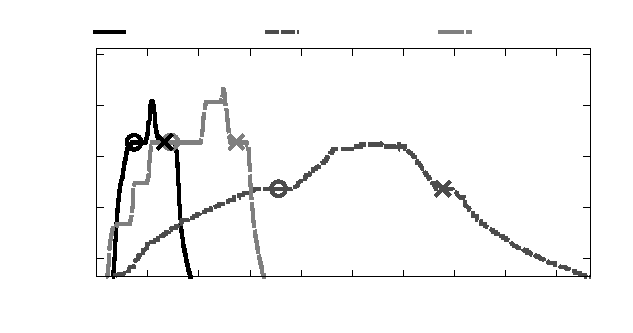
\includegraphics{SCCRuleFat}}%
    \gplfronttext
  \end{picture}%
\endgroup
}}
    \caption{SCC}
    \label{fig:rule_number:fat:scc}
  \end{subfigure}
  \par\bigskip
  \begin{subfigure}[b]{0.69\linewidth}
    \resizebox{\textwidth}{!}{\footnotesize{% GNUPLOT: LaTeX picture with Postscript
\begingroup
  \fontfamily{Times-Roman}%
  \selectfont
  \makeatletter
  \providecommand\color[2][]{%
    \GenericError{(gnuplot) \space\space\space\@spaces}{%
      Package color not loaded in conjunction with
      terminal option `colourtext'%
    }{See the gnuplot documentation for explanation.%
    }{Either use 'blacktext' in gnuplot or load the package
      color.sty in LaTeX.}%
    \renewcommand\color[2][]{}%
  }%
  \providecommand\includegraphics[2][]{%
    \GenericError{(gnuplot) \space\space\space\@spaces}{%
      Package graphicx or graphics not loaded%
    }{See the gnuplot documentation for explanation.%
    }{The gnuplot epslatex terminal needs graphicx.sty or graphics.sty.}%
    \renewcommand\includegraphics[2][]{}%
  }%
  \providecommand\rotatebox[2]{#2}%
  \@ifundefined{ifGPcolor}{%
    \newif\ifGPcolor
    \GPcolortrue
  }{}%
  \@ifundefined{ifGPblacktext}{%
    \newif\ifGPblacktext
    \GPblacktexttrue
  }{}%
  % define a \g@addto@macro without @ in the name:
  \let\gplgaddtomacro\g@addto@macro
  % define empty templates for all commands taking text:
  \gdef\gplbacktext{}%
  \gdef\gplfronttext{}%
  \makeatother
  \ifGPblacktext
    % no textcolor at all
    \def\colorrgb#1{}%
    \def\colorgray#1{}%
  \else
    % gray or color?
    \ifGPcolor
      \def\colorrgb#1{\color[rgb]{#1}}%
      \def\colorgray#1{\color[gray]{#1}}%
      \expandafter\def\csname LTw\endcsname{\color{white}}%
      \expandafter\def\csname LTb\endcsname{\color{black}}%
      \expandafter\def\csname LTa\endcsname{\color{black}}%
      \expandafter\def\csname LT0\endcsname{\color[rgb]{1,0,0}}%
      \expandafter\def\csname LT1\endcsname{\color[rgb]{0,1,0}}%
      \expandafter\def\csname LT2\endcsname{\color[rgb]{0,0,1}}%
      \expandafter\def\csname LT3\endcsname{\color[rgb]{1,0,1}}%
      \expandafter\def\csname LT4\endcsname{\color[rgb]{0,1,1}}%
      \expandafter\def\csname LT5\endcsname{\color[rgb]{1,1,0}}%
      \expandafter\def\csname LT6\endcsname{\color[rgb]{0,0,0}}%
      \expandafter\def\csname LT7\endcsname{\color[rgb]{1,0.3,0}}%
      \expandafter\def\csname LT8\endcsname{\color[rgb]{0.5,0.5,0.5}}%
    \else
      % gray
      \def\colorrgb#1{\color{black}}%
      \def\colorgray#1{\color[gray]{#1}}%
      \expandafter\def\csname LTw\endcsname{\color{white}}%
      \expandafter\def\csname LTb\endcsname{\color{black}}%
      \expandafter\def\csname LTa\endcsname{\color{black}}%
      \expandafter\def\csname LT0\endcsname{\color{black}}%
      \expandafter\def\csname LT1\endcsname{\color{black}}%
      \expandafter\def\csname LT2\endcsname{\color{black}}%
      \expandafter\def\csname LT3\endcsname{\color{black}}%
      \expandafter\def\csname LT4\endcsname{\color{black}}%
      \expandafter\def\csname LT5\endcsname{\color{black}}%
      \expandafter\def\csname LT6\endcsname{\color{black}}%
      \expandafter\def\csname LT7\endcsname{\color{black}}%
      \expandafter\def\csname LT8\endcsname{\color{black}}%
    \fi
  \fi
    \setlength{\unitlength}{0.0500bp}%
    \ifx\gptboxheight\undefined%
      \newlength{\gptboxheight}%
      \newlength{\gptboxwidth}%
      \newsavebox{\gptboxtext}%
    \fi%
    \setlength{\fboxrule}{0.5pt}%
    \setlength{\fboxsep}{1pt}%
\begin{picture}(5760.00,2880.00)%
    \gplgaddtomacro\gplbacktext{%
      \csname LTb\endcsname%%
      \put(686,588){\makebox(0,0)[r]{\strut{}$12300$}}%
      \put(686,1039){\makebox(0,0)[r]{\strut{}$12600$}}%
      \put(686,1490){\makebox(0,0)[r]{\strut{}$12900$}}%
      \put(686,1940){\makebox(0,0)[r]{\strut{}$13200$}}%
      \put(686,2391){\makebox(0,0)[r]{\strut{}$13500$}}%
      \put(770,252){\makebox(0,0){\strut{}$0$}}%
      \put(1557,252){\makebox(0,0){\strut{}$1000$}}%
      \put(2344,252){\makebox(0,0){\strut{}$2000$}}%
      \put(3130,252){\makebox(0,0){\strut{}$3000$}}%
      \put(3917,252){\makebox(0,0){\strut{}$4000$}}%
      \put(4704,252){\makebox(0,0){\strut{}$5000$}}%
      \put(5491,252){\makebox(0,0){\strut{}$6000$}}%
    }%
    \gplgaddtomacro\gplfronttext{%
      \csname LTb\endcsname%%
      \put(168,1474){\rotatebox{-270}{\makebox(0,0){\strut{}Total number of rules}}}%
      \put(3138,98){\makebox(0,0){\strut{}Time (ms)}}%
      \csname LTb\endcsname%%
      \put(1259,2733){\makebox(0,0)[l]{\strut{}CU+Nimble}}%
      \csname LTb\endcsname%%
      \put(2834,2733){\makebox(0,0)[l]{\strut{}CU+OpenNF}}%
      \csname LTb\endcsname%%
      \put(4409,2733){\makebox(0,0)[l]{\strut{}CU+SwingState}}%
    }%
    \gplbacktext
    \put(0,0){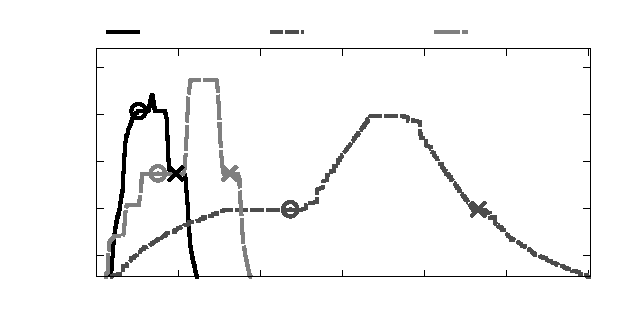
\includegraphics{CURuleFat}}%
    \gplfronttext
  \end{picture}%
\endgroup
}}
    \caption{CU}
    \label{fig:rule_number:fat:scc}
  \end{subfigure}
  \par\bigskip
  \begin{subfigure}[b]{0.69\linewidth}
    \resizebox{\textwidth}{!}{\footnotesize{% GNUPLOT: LaTeX picture with Postscript
\begingroup
  \fontfamily{Times-Roman}%
  \selectfont
  \makeatletter
  \providecommand\color[2][]{%
    \GenericError{(gnuplot) \space\space\space\@spaces}{%
      Package color not loaded in conjunction with
      terminal option `colourtext'%
    }{See the gnuplot documentation for explanation.%
    }{Either use 'blacktext' in gnuplot or load the package
      color.sty in LaTeX.}%
    \renewcommand\color[2][]{}%
  }%
  \providecommand\includegraphics[2][]{%
    \GenericError{(gnuplot) \space\space\space\@spaces}{%
      Package graphicx or graphics not loaded%
    }{See the gnuplot documentation for explanation.%
    }{The gnuplot epslatex terminal needs graphicx.sty or graphics.sty.}%
    \renewcommand\includegraphics[2][]{}%
  }%
  \providecommand\rotatebox[2]{#2}%
  \@ifundefined{ifGPcolor}{%
    \newif\ifGPcolor
    \GPcolortrue
  }{}%
  \@ifundefined{ifGPblacktext}{%
    \newif\ifGPblacktext
    \GPblacktexttrue
  }{}%
  % define a \g@addto@macro without @ in the name:
  \let\gplgaddtomacro\g@addto@macro
  % define empty templates for all commands taking text:
  \gdef\gplbacktext{}%
  \gdef\gplfronttext{}%
  \makeatother
  \ifGPblacktext
    % no textcolor at all
    \def\colorrgb#1{}%
    \def\colorgray#1{}%
  \else
    % gray or color?
    \ifGPcolor
      \def\colorrgb#1{\color[rgb]{#1}}%
      \def\colorgray#1{\color[gray]{#1}}%
      \expandafter\def\csname LTw\endcsname{\color{white}}%
      \expandafter\def\csname LTb\endcsname{\color{black}}%
      \expandafter\def\csname LTa\endcsname{\color{black}}%
      \expandafter\def\csname LT0\endcsname{\color[rgb]{1,0,0}}%
      \expandafter\def\csname LT1\endcsname{\color[rgb]{0,1,0}}%
      \expandafter\def\csname LT2\endcsname{\color[rgb]{0,0,1}}%
      \expandafter\def\csname LT3\endcsname{\color[rgb]{1,0,1}}%
      \expandafter\def\csname LT4\endcsname{\color[rgb]{0,1,1}}%
      \expandafter\def\csname LT5\endcsname{\color[rgb]{1,1,0}}%
      \expandafter\def\csname LT6\endcsname{\color[rgb]{0,0,0}}%
      \expandafter\def\csname LT7\endcsname{\color[rgb]{1,0.3,0}}%
      \expandafter\def\csname LT8\endcsname{\color[rgb]{0.5,0.5,0.5}}%
    \else
      % gray
      \def\colorrgb#1{\color{black}}%
      \def\colorgray#1{\color[gray]{#1}}%
      \expandafter\def\csname LTw\endcsname{\color{white}}%
      \expandafter\def\csname LTb\endcsname{\color{black}}%
      \expandafter\def\csname LTa\endcsname{\color{black}}%
      \expandafter\def\csname LT0\endcsname{\color{black}}%
      \expandafter\def\csname LT1\endcsname{\color{black}}%
      \expandafter\def\csname LT2\endcsname{\color{black}}%
      \expandafter\def\csname LT3\endcsname{\color{black}}%
      \expandafter\def\csname LT4\endcsname{\color{black}}%
      \expandafter\def\csname LT5\endcsname{\color{black}}%
      \expandafter\def\csname LT6\endcsname{\color{black}}%
      \expandafter\def\csname LT7\endcsname{\color{black}}%
      \expandafter\def\csname LT8\endcsname{\color{black}}%
    \fi
  \fi
    \setlength{\unitlength}{0.0500bp}%
    \ifx\gptboxheight\undefined%
      \newlength{\gptboxheight}%
      \newlength{\gptboxwidth}%
      \newsavebox{\gptboxtext}%
    \fi%
    \setlength{\fboxrule}{0.5pt}%
    \setlength{\fboxsep}{1pt}%
\begin{picture}(5760.00,2880.00)%
    \gplgaddtomacro\gplbacktext{%
      \csname LTb\endcsname%%
      \put(686,547){\makebox(0,0)[r]{\strut{}$12250$}}%
      \put(686,1015){\makebox(0,0)[r]{\strut{}$12500$}}%
      \put(686,1484){\makebox(0,0)[r]{\strut{}$12750$}}%
      \put(686,1952){\makebox(0,0)[r]{\strut{}$13000$}}%
      \put(686,2421){\makebox(0,0)[r]{\strut{}$13250$}}%
      \put(770,252){\makebox(0,0){\strut{}$0$}}%
      \put(1272,252){\makebox(0,0){\strut{}$500$}}%
      \put(1775,252){\makebox(0,0){\strut{}$1000$}}%
      \put(2277,252){\makebox(0,0){\strut{}$1500$}}%
      \put(2780,252){\makebox(0,0){\strut{}$2000$}}%
      \put(3282,252){\makebox(0,0){\strut{}$2500$}}%
      \put(3785,252){\makebox(0,0){\strut{}$3000$}}%
      \put(4287,252){\makebox(0,0){\strut{}$3500$}}%
      \put(4790,252){\makebox(0,0){\strut{}$4000$}}%
      \put(5292,252){\makebox(0,0){\strut{}$4500$}}%
    }%
    \gplgaddtomacro\gplfronttext{%
      \csname LTb\endcsname%%
      \put(168,1474){\rotatebox{-270}{\makebox(0,0){\strut{}Total number of rules}}}%
      \put(3138,98){\makebox(0,0){\strut{}Time (ms)}}%
      \csname LTb\endcsname%%
      \put(1133,2733){\makebox(0,0)[l]{\strut{}RWC+Nimble}}%
      \csname LTb\endcsname%%
      \put(2792,2733){\makebox(0,0)[l]{\strut{}RWC+OpenNF}}%
      \csname LTb\endcsname%%
      \put(4451,2733){\makebox(0,0)[l]{\strut{}RWC+SwingState}}%
    }%
    \gplbacktext
    \put(0,0){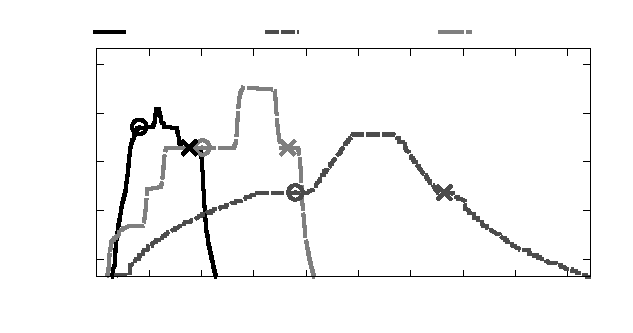
\includegraphics{RWCRuleFat}}%
    \gplfronttext
  \end{picture}%
\endgroup
}}
    \caption{\ourRouteUpdateName}
    \label{fig:rule_number:fat:cu}
  \end{subfigure}
  \caption{Rules in the network during 100 path changes and
    accompanying NF migrations for fat-tree topology; markers show
    completion of path changes ($\times$) and NF migrations
    ({\LARGE $\circ$})}
\label{fig:rule_number:fat}
\end{figure}



\subsection{Memory Overhead in Switches}


To evaluate the number of rules (including rules to build tunnels)
imposed on the switches by each algorithm, we examined the per-switch
logs of rule installations and deletions over 100 consecutive path
changes in the fat-tree topology ($\portsPerSwitch = 8$). We computed
a time series of the total number of rules installed across all
switches in the network, including the time cleaning up tunnels used
to migrate NFs and to tunnel traffic. This time series for a
representative run of each of SCC, CU, and \ourRouteUpdateName using
\sysname, SwingState and OpenNF is shown in
\figref{fig:rule_number:fat}.  We repeated this evaluation on the
Forthnet topology, but by breaking the busiest link; see
\figref{fig:rule_number:Forthnet}.  Each curve is marked with the time
when NF migration for all flows was done and the time when all path
changes were completed.  All three algorithms require installing rules
on \oldSwitchID{\nfIdx} and \newSwitchID{\nfIdx} to deal with incoming
packets and also to clean up these rules.  Different from OpenNF,
\sysname and SwingState need to build tunnels to migrate NFs and to
tunnel traffic.  As these figures show, \sysname requires less time to
finish NF migrations and path changes, because it performs both
operations simultaneously. OpenNF needs more time to finish path changes
than SwingState since OpenNF buffers and redistributes all incoming packets in the controller,
which induces a large delay before path change can be executed.


\begin{figure}[H]
\centering
   \begin{subfigure}[b]{0.69\linewidth}
    \resizebox{\textwidth}{!}{\footnotesize{% GNUPLOT: LaTeX picture with Postscript
\begingroup
  \fontfamily{Times-Roman}%
  \selectfont
  \makeatletter
  \providecommand\color[2][]{%
    \GenericError{(gnuplot) \space\space\space\@spaces}{%
      Package color not loaded in conjunction with
      terminal option `colourtext'%
    }{See the gnuplot documentation for explanation.%
    }{Either use 'blacktext' in gnuplot or load the package
      color.sty in LaTeX.}%
    \renewcommand\color[2][]{}%
  }%
  \providecommand\includegraphics[2][]{%
    \GenericError{(gnuplot) \space\space\space\@spaces}{%
      Package graphicx or graphics not loaded%
    }{See the gnuplot documentation for explanation.%
    }{The gnuplot epslatex terminal needs graphicx.sty or graphics.sty.}%
    \renewcommand\includegraphics[2][]{}%
  }%
  \providecommand\rotatebox[2]{#2}%
  \@ifundefined{ifGPcolor}{%
    \newif\ifGPcolor
    \GPcolortrue
  }{}%
  \@ifundefined{ifGPblacktext}{%
    \newif\ifGPblacktext
    \GPblacktexttrue
  }{}%
  % define a \g@addto@macro without @ in the name:
  \let\gplgaddtomacro\g@addto@macro
  % define empty templates for all commands taking text:
  \gdef\gplbacktext{}%
  \gdef\gplfronttext{}%
  \makeatother
  \ifGPblacktext
    % no textcolor at all
    \def\colorrgb#1{}%
    \def\colorgray#1{}%
  \else
    % gray or color?
    \ifGPcolor
      \def\colorrgb#1{\color[rgb]{#1}}%
      \def\colorgray#1{\color[gray]{#1}}%
      \expandafter\def\csname LTw\endcsname{\color{white}}%
      \expandafter\def\csname LTb\endcsname{\color{black}}%
      \expandafter\def\csname LTa\endcsname{\color{black}}%
      \expandafter\def\csname LT0\endcsname{\color[rgb]{1,0,0}}%
      \expandafter\def\csname LT1\endcsname{\color[rgb]{0,1,0}}%
      \expandafter\def\csname LT2\endcsname{\color[rgb]{0,0,1}}%
      \expandafter\def\csname LT3\endcsname{\color[rgb]{1,0,1}}%
      \expandafter\def\csname LT4\endcsname{\color[rgb]{0,1,1}}%
      \expandafter\def\csname LT5\endcsname{\color[rgb]{1,1,0}}%
      \expandafter\def\csname LT6\endcsname{\color[rgb]{0,0,0}}%
      \expandafter\def\csname LT7\endcsname{\color[rgb]{1,0.3,0}}%
      \expandafter\def\csname LT8\endcsname{\color[rgb]{0.5,0.5,0.5}}%
    \else
      % gray
      \def\colorrgb#1{\color{black}}%
      \def\colorgray#1{\color[gray]{#1}}%
      \expandafter\def\csname LTw\endcsname{\color{white}}%
      \expandafter\def\csname LTb\endcsname{\color{black}}%
      \expandafter\def\csname LTa\endcsname{\color{black}}%
      \expandafter\def\csname LT0\endcsname{\color{black}}%
      \expandafter\def\csname LT1\endcsname{\color{black}}%
      \expandafter\def\csname LT2\endcsname{\color{black}}%
      \expandafter\def\csname LT3\endcsname{\color{black}}%
      \expandafter\def\csname LT4\endcsname{\color{black}}%
      \expandafter\def\csname LT5\endcsname{\color{black}}%
      \expandafter\def\csname LT6\endcsname{\color{black}}%
      \expandafter\def\csname LT7\endcsname{\color{black}}%
      \expandafter\def\csname LT8\endcsname{\color{black}}%
    \fi
  \fi
    \setlength{\unitlength}{0.0500bp}%
    \ifx\gptboxheight\undefined%
      \newlength{\gptboxheight}%
      \newlength{\gptboxwidth}%
      \newsavebox{\gptboxtext}%
    \fi%
    \setlength{\fboxrule}{0.5pt}%
    \setlength{\fboxsep}{1pt}%
\begin{picture}(5760.00,2880.00)%
    \gplgaddtomacro\gplbacktext{%
      \csname LTb\endcsname%%
      \put(686,553){\makebox(0,0)[r]{\strut{}$12000$}}%
      \put(686,1005){\makebox(0,0)[r]{\strut{}$12400$}}%
      \put(686,1456){\makebox(0,0)[r]{\strut{}$12800$}}%
      \put(686,1908){\makebox(0,0)[r]{\strut{}$13200$}}%
      \put(686,2360){\makebox(0,0)[r]{\strut{}$13600$}}%
      \put(770,252){\makebox(0,0){\strut{}$0$}}%
      \put(1627,252){\makebox(0,0){\strut{}$2000$}}%
      \put(2483,252){\makebox(0,0){\strut{}$4000$}}%
      \put(3340,252){\makebox(0,0){\strut{}$6000$}}%
      \put(4197,252){\makebox(0,0){\strut{}$8000$}}%
      \put(5053,252){\makebox(0,0){\strut{}$10000$}}%
    }%
    \gplgaddtomacro\gplfronttext{%
      \csname LTb\endcsname%%
      \put(168,1474){\rotatebox{-270}{\makebox(0,0){\strut{}Total number of rules}}}%
      \put(3138,98){\makebox(0,0){\strut{}Time (ms)}}%
      \csname LTb\endcsname%%
      \put(1133,2733){\makebox(0,0)[l]{\strut{}SCC+Nimble}}%
      \csname LTb\endcsname%%
      \put(2792,2733){\makebox(0,0)[l]{\strut{}SCC+OpenNF}}%
      \csname LTb\endcsname%%
      \put(4451,2733){\makebox(0,0)[l]{\strut{}SCC+SwingState}}%
    }%
    \gplbacktext
    \put(0,0){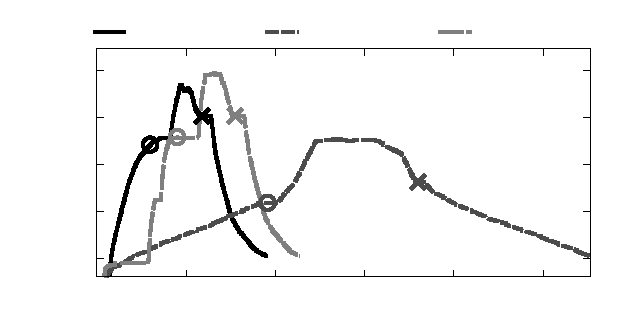
\includegraphics{SCCRuleForthnet}}%
    \gplfronttext
  \end{picture}%
\endgroup
}}
    \caption{SCC}
    \label{fig:rule_number:Forthnet:scc}
  \end{subfigure}
  \par\bigskip
  \begin{subfigure}[b]{0.69\linewidth}
    \resizebox{\textwidth}{!}{\footnotesize{% GNUPLOT: LaTeX picture with Postscript
\begingroup
  \fontfamily{Times-Roman}%
  \selectfont
  \makeatletter
  \providecommand\color[2][]{%
    \GenericError{(gnuplot) \space\space\space\@spaces}{%
      Package color not loaded in conjunction with
      terminal option `colourtext'%
    }{See the gnuplot documentation for explanation.%
    }{Either use 'blacktext' in gnuplot or load the package
      color.sty in LaTeX.}%
    \renewcommand\color[2][]{}%
  }%
  \providecommand\includegraphics[2][]{%
    \GenericError{(gnuplot) \space\space\space\@spaces}{%
      Package graphicx or graphics not loaded%
    }{See the gnuplot documentation for explanation.%
    }{The gnuplot epslatex terminal needs graphicx.sty or graphics.sty.}%
    \renewcommand\includegraphics[2][]{}%
  }%
  \providecommand\rotatebox[2]{#2}%
  \@ifundefined{ifGPcolor}{%
    \newif\ifGPcolor
    \GPcolortrue
  }{}%
  \@ifundefined{ifGPblacktext}{%
    \newif\ifGPblacktext
    \GPblacktexttrue
  }{}%
  % define a \g@addto@macro without @ in the name:
  \let\gplgaddtomacro\g@addto@macro
  % define empty templates for all commands taking text:
  \gdef\gplbacktext{}%
  \gdef\gplfronttext{}%
  \makeatother
  \ifGPblacktext
    % no textcolor at all
    \def\colorrgb#1{}%
    \def\colorgray#1{}%
  \else
    % gray or color?
    \ifGPcolor
      \def\colorrgb#1{\color[rgb]{#1}}%
      \def\colorgray#1{\color[gray]{#1}}%
      \expandafter\def\csname LTw\endcsname{\color{white}}%
      \expandafter\def\csname LTb\endcsname{\color{black}}%
      \expandafter\def\csname LTa\endcsname{\color{black}}%
      \expandafter\def\csname LT0\endcsname{\color[rgb]{1,0,0}}%
      \expandafter\def\csname LT1\endcsname{\color[rgb]{0,1,0}}%
      \expandafter\def\csname LT2\endcsname{\color[rgb]{0,0,1}}%
      \expandafter\def\csname LT3\endcsname{\color[rgb]{1,0,1}}%
      \expandafter\def\csname LT4\endcsname{\color[rgb]{0,1,1}}%
      \expandafter\def\csname LT5\endcsname{\color[rgb]{1,1,0}}%
      \expandafter\def\csname LT6\endcsname{\color[rgb]{0,0,0}}%
      \expandafter\def\csname LT7\endcsname{\color[rgb]{1,0.3,0}}%
      \expandafter\def\csname LT8\endcsname{\color[rgb]{0.5,0.5,0.5}}%
    \else
      % gray
      \def\colorrgb#1{\color{black}}%
      \def\colorgray#1{\color[gray]{#1}}%
      \expandafter\def\csname LTw\endcsname{\color{white}}%
      \expandafter\def\csname LTb\endcsname{\color{black}}%
      \expandafter\def\csname LTa\endcsname{\color{black}}%
      \expandafter\def\csname LT0\endcsname{\color{black}}%
      \expandafter\def\csname LT1\endcsname{\color{black}}%
      \expandafter\def\csname LT2\endcsname{\color{black}}%
      \expandafter\def\csname LT3\endcsname{\color{black}}%
      \expandafter\def\csname LT4\endcsname{\color{black}}%
      \expandafter\def\csname LT5\endcsname{\color{black}}%
      \expandafter\def\csname LT6\endcsname{\color{black}}%
      \expandafter\def\csname LT7\endcsname{\color{black}}%
      \expandafter\def\csname LT8\endcsname{\color{black}}%
    \fi
  \fi
    \setlength{\unitlength}{0.0500bp}%
    \ifx\gptboxheight\undefined%
      \newlength{\gptboxheight}%
      \newlength{\gptboxwidth}%
      \newsavebox{\gptboxtext}%
    \fi%
    \setlength{\fboxrule}{0.5pt}%
    \setlength{\fboxsep}{1pt}%
\begin{picture}(5760.00,2880.00)%
    \gplgaddtomacro\gplbacktext{%
      \csname LTb\endcsname%%
      \put(686,417){\makebox(0,0)[r]{\strut{}$11900$}}%
      \put(686,920){\makebox(0,0)[r]{\strut{}$12600$}}%
      \put(686,1422){\makebox(0,0)[r]{\strut{}$13300$}}%
      \put(686,1924){\makebox(0,0)[r]{\strut{}$14000$}}%
      \put(686,2427){\makebox(0,0)[r]{\strut{}$14700$}}%
      \put(770,252){\makebox(0,0){\strut{}$0$}}%
      \put(1509,252){\makebox(0,0){\strut{}$2000$}}%
      \put(2248,252){\makebox(0,0){\strut{}$4000$}}%
      \put(2986,252){\makebox(0,0){\strut{}$6000$}}%
      \put(3725,252){\makebox(0,0){\strut{}$8000$}}%
      \put(4464,252){\makebox(0,0){\strut{}$10000$}}%
      \put(5203,252){\makebox(0,0){\strut{}$12000$}}%
    }%
    \gplgaddtomacro\gplfronttext{%
      \csname LTb\endcsname%%
      \put(168,1474){\rotatebox{-270}{\makebox(0,0){\strut{}Total number of rules}}}%
      \put(3138,98){\makebox(0,0){\strut{}Time (ms)}}%
      \csname LTb\endcsname%%
      \put(1259,2733){\makebox(0,0)[l]{\strut{}CU+Nimble}}%
      \csname LTb\endcsname%%
      \put(2834,2733){\makebox(0,0)[l]{\strut{}CU+OpenNF}}%
      \csname LTb\endcsname%%
      \put(4409,2733){\makebox(0,0)[l]{\strut{}CU+SwingState}}%
    }%
    \gplbacktext
    \put(0,0){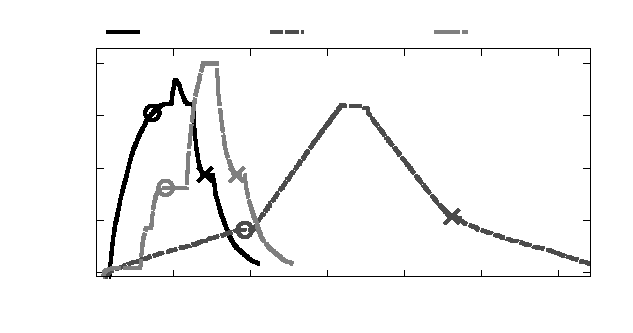
\includegraphics{CURuleForthnet}}%
    \gplfronttext
  \end{picture}%
\endgroup
}}
    \caption{CU}
    \label{fig:rule_number:Forthnet:scc}
  \end{subfigure}
  \par\bigskip
  \begin{subfigure}[b]{0.69\linewidth}
    \resizebox{\textwidth}{!}{\small{% GNUPLOT: LaTeX picture with Postscript
\begingroup
  \fontfamily{Times-Roman}%
  \selectfont
  \makeatletter
  \providecommand\color[2][]{%
    \GenericError{(gnuplot) \space\space\space\@spaces}{%
      Package color not loaded in conjunction with
      terminal option `colourtext'%
    }{See the gnuplot documentation for explanation.%
    }{Either use 'blacktext' in gnuplot or load the package
      color.sty in LaTeX.}%
    \renewcommand\color[2][]{}%
  }%
  \providecommand\includegraphics[2][]{%
    \GenericError{(gnuplot) \space\space\space\@spaces}{%
      Package graphicx or graphics not loaded%
    }{See the gnuplot documentation for explanation.%
    }{The gnuplot epslatex terminal needs graphicx.sty or graphics.sty.}%
    \renewcommand\includegraphics[2][]{}%
  }%
  \providecommand\rotatebox[2]{#2}%
  \@ifundefined{ifGPcolor}{%
    \newif\ifGPcolor
    \GPcolortrue
  }{}%
  \@ifundefined{ifGPblacktext}{%
    \newif\ifGPblacktext
    \GPblacktexttrue
  }{}%
  % define a \g@addto@macro without @ in the name:
  \let\gplgaddtomacro\g@addto@macro
  % define empty templates for all commands taking text:
  \gdef\gplbacktext{}%
  \gdef\gplfronttext{}%
  \makeatother
  \ifGPblacktext
    % no textcolor at all
    \def\colorrgb#1{}%
    \def\colorgray#1{}%
  \else
    % gray or color?
    \ifGPcolor
      \def\colorrgb#1{\color[rgb]{#1}}%
      \def\colorgray#1{\color[gray]{#1}}%
      \expandafter\def\csname LTw\endcsname{\color{white}}%
      \expandafter\def\csname LTb\endcsname{\color{black}}%
      \expandafter\def\csname LTa\endcsname{\color{black}}%
      \expandafter\def\csname LT0\endcsname{\color[rgb]{1,0,0}}%
      \expandafter\def\csname LT1\endcsname{\color[rgb]{0,1,0}}%
      \expandafter\def\csname LT2\endcsname{\color[rgb]{0,0,1}}%
      \expandafter\def\csname LT3\endcsname{\color[rgb]{1,0,1}}%
      \expandafter\def\csname LT4\endcsname{\color[rgb]{0,1,1}}%
      \expandafter\def\csname LT5\endcsname{\color[rgb]{1,1,0}}%
      \expandafter\def\csname LT6\endcsname{\color[rgb]{0,0,0}}%
      \expandafter\def\csname LT7\endcsname{\color[rgb]{1,0.3,0}}%
      \expandafter\def\csname LT8\endcsname{\color[rgb]{0.5,0.5,0.5}}%
    \else
      % gray
      \def\colorrgb#1{\color{black}}%
      \def\colorgray#1{\color[gray]{#1}}%
      \expandafter\def\csname LTw\endcsname{\color{white}}%
      \expandafter\def\csname LTb\endcsname{\color{black}}%
      \expandafter\def\csname LTa\endcsname{\color{black}}%
      \expandafter\def\csname LT0\endcsname{\color{black}}%
      \expandafter\def\csname LT1\endcsname{\color{black}}%
      \expandafter\def\csname LT2\endcsname{\color{black}}%
      \expandafter\def\csname LT3\endcsname{\color{black}}%
      \expandafter\def\csname LT4\endcsname{\color{black}}%
      \expandafter\def\csname LT5\endcsname{\color{black}}%
      \expandafter\def\csname LT6\endcsname{\color{black}}%
      \expandafter\def\csname LT7\endcsname{\color{black}}%
      \expandafter\def\csname LT8\endcsname{\color{black}}%
    \fi
  \fi
    \setlength{\unitlength}{0.0500bp}%
    \ifx\gptboxheight\undefined%
      \newlength{\gptboxheight}%
      \newlength{\gptboxwidth}%
      \newsavebox{\gptboxtext}%
    \fi%
    \setlength{\fboxrule}{0.5pt}%
    \setlength{\fboxsep}{1pt}%
\begin{picture}(5760.00,2880.00)%
    \gplgaddtomacro\gplbacktext{%
      \csname LTb\endcsname%%
      \put(686,540){\makebox(0,0)[r]{\strut{}$12000$}}%
      \put(686,1061){\makebox(0,0)[r]{\strut{}$12500$}}%
      \put(686,1582){\makebox(0,0)[r]{\strut{}$13000$}}%
      \put(686,2104){\makebox(0,0)[r]{\strut{}$13500$}}%
      \put(770,252){\makebox(0,0){\strut{}$0$}}%
      \put(1716,252){\makebox(0,0){\strut{}$2000$}}%
      \put(2662,252){\makebox(0,0){\strut{}$4000$}}%
      \put(3608,252){\makebox(0,0){\strut{}$6000$}}%
      \put(4554,252){\makebox(0,0){\strut{}$8000$}}%
      \put(5500,252){\makebox(0,0){\strut{}$10000$}}%
    }%
    \gplgaddtomacro\gplfronttext{%
      \csname LTb\endcsname%%
      \put(168,1474){\rotatebox{-270}{\makebox(0,0){\strut{}Total number of rules}}}%
      \put(3138,98){\makebox(0,0){\strut{}Time (ms)}}%
      \csname LTb\endcsname%%
      \put(1133,2733){\makebox(0,0)[l]{\strut{}RWC+Nimble}}%
      \csname LTb\endcsname%%
      \put(2792,2733){\makebox(0,0)[l]{\strut{}RWC+OpenNF}}%
      \csname LTb\endcsname%%
      \put(4451,2733){\makebox(0,0)[l]{\strut{}RWC+SwingState}}%
    }%
    \gplbacktext
    \put(0,0){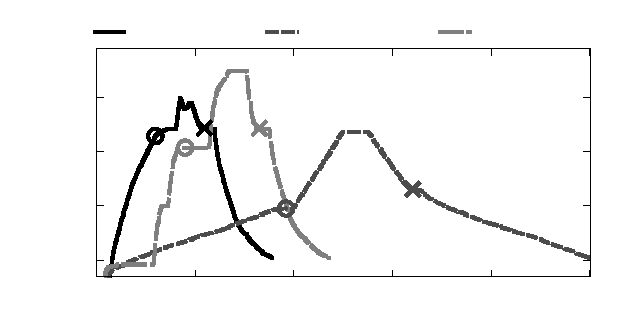
\includegraphics{RWCRuleForthnet}}%
    \gplfronttext
  \end{picture}%
\endgroup
}}
    \caption{\ourRouteUpdateName}
    \label{fig:rule_number:Forthnet:cu}
  \end{subfigure}
  \caption{Rules in the network during 178 path changes and
    accompanying NF migrations for Forthnet topology; markers show
    completion of path changes ($\times$) and NF migrations
    ({\LARGE $\circ$})}
\label{fig:rule_number:Forthnet}
\end{figure}



\subsection{Packet Latency During Link Failure}

To evaluate the latency imposed on each flow upon link failure by each
algorithm, we measured the time required for a destination host to
receive $10\megabytes$ from a source host through a TCP connection. We
broke one random link and selected $10$ flows to update their routing
polices.  The source host of each flow started to send a stream of
packets at speed $100\megabits/\sec$ to the destination host upon link
failure. The time shown in \figref{fig:latency} shows the times for
the destination to receive $10\megabytes$ using each
algorithm. \sysname outperforms SwingState and OpenNF because \sysname
recovers the new path more efficiently by performing NF migration and
path update simultaneously.  Though SwingState also uses tunnels to
migrate NFs, it mirrors packets but still delivers packets through
the old path during NF migration.  Plus, OpenNF uses a single
controller to redistribute incoming packets, which significantly slows
down the speed.

\begin{figure}[t]
\centering
 \begin{subfigure}[b]{0.7\columnwidth}
    \resizebox{\textwidth}{!}{\footnotesize{% GNUPLOT: LaTeX picture with Postscript
\begingroup
  \fontfamily{Times-Roman}%
  \selectfont
  \makeatletter
  \providecommand\color[2][]{%
    \GenericError{(gnuplot) \space\space\space\@spaces}{%
      Package color not loaded in conjunction with
      terminal option `colourtext'%
    }{See the gnuplot documentation for explanation.%
    }{Either use 'blacktext' in gnuplot or load the package
      color.sty in LaTeX.}%
    \renewcommand\color[2][]{}%
  }%
  \providecommand\includegraphics[2][]{%
    \GenericError{(gnuplot) \space\space\space\@spaces}{%
      Package graphicx or graphics not loaded%
    }{See the gnuplot documentation for explanation.%
    }{The gnuplot epslatex terminal needs graphicx.sty or graphics.sty.}%
    \renewcommand\includegraphics[2][]{}%
  }%
  \providecommand\rotatebox[2]{#2}%
  \@ifundefined{ifGPcolor}{%
    \newif\ifGPcolor
    \GPcolortrue
  }{}%
  \@ifundefined{ifGPblacktext}{%
    \newif\ifGPblacktext
    \GPblacktexttrue
  }{}%
  % define a \g@addto@macro without @ in the name:
  \let\gplgaddtomacro\g@addto@macro
  % define empty templates for all commands taking text:
  \gdef\gplbacktext{}%
  \gdef\gplfronttext{}%
  \makeatother
  \ifGPblacktext
    % no textcolor at all
    \def\colorrgb#1{}%
    \def\colorgray#1{}%
  \else
    % gray or color?
    \ifGPcolor
      \def\colorrgb#1{\color[rgb]{#1}}%
      \def\colorgray#1{\color[gray]{#1}}%
      \expandafter\def\csname LTw\endcsname{\color{white}}%
      \expandafter\def\csname LTb\endcsname{\color{black}}%
      \expandafter\def\csname LTa\endcsname{\color{black}}%
      \expandafter\def\csname LT0\endcsname{\color[rgb]{1,0,0}}%
      \expandafter\def\csname LT1\endcsname{\color[rgb]{0,1,0}}%
      \expandafter\def\csname LT2\endcsname{\color[rgb]{0,0,1}}%
      \expandafter\def\csname LT3\endcsname{\color[rgb]{1,0,1}}%
      \expandafter\def\csname LT4\endcsname{\color[rgb]{0,1,1}}%
      \expandafter\def\csname LT5\endcsname{\color[rgb]{1,1,0}}%
      \expandafter\def\csname LT6\endcsname{\color[rgb]{0,0,0}}%
      \expandafter\def\csname LT7\endcsname{\color[rgb]{1,0.3,0}}%
      \expandafter\def\csname LT8\endcsname{\color[rgb]{0.5,0.5,0.5}}%
    \else
      % gray
      \def\colorrgb#1{\color{black}}%
      \def\colorgray#1{\color[gray]{#1}}%
      \expandafter\def\csname LTw\endcsname{\color{white}}%
      \expandafter\def\csname LTb\endcsname{\color{black}}%
      \expandafter\def\csname LTa\endcsname{\color{black}}%
      \expandafter\def\csname LT0\endcsname{\color{black}}%
      \expandafter\def\csname LT1\endcsname{\color{black}}%
      \expandafter\def\csname LT2\endcsname{\color{black}}%
      \expandafter\def\csname LT3\endcsname{\color{black}}%
      \expandafter\def\csname LT4\endcsname{\color{black}}%
      \expandafter\def\csname LT5\endcsname{\color{black}}%
      \expandafter\def\csname LT6\endcsname{\color{black}}%
      \expandafter\def\csname LT7\endcsname{\color{black}}%
      \expandafter\def\csname LT8\endcsname{\color{black}}%
    \fi
  \fi
    \setlength{\unitlength}{0.0500bp}%
    \ifx\gptboxheight\undefined%
      \newlength{\gptboxheight}%
      \newlength{\gptboxwidth}%
      \newsavebox{\gptboxtext}%
    \fi%
    \setlength{\fboxrule}{0.5pt}%
    \setlength{\fboxsep}{1pt}%
\begin{picture}(7200.00,2880.00)%
    \gplgaddtomacro\gplbacktext{%
      \csname LTb\endcsname%%
      \put(782,528){\makebox(0,0)[r]{\strut{}$1100$}}%
      \csname LTb\endcsname%%
      \put(782,1089){\makebox(0,0)[r]{\strut{}$1110$}}%
      \csname LTb\endcsname%%
      \put(782,1651){\makebox(0,0)[r]{\strut{}$1120$}}%
      \csname LTb\endcsname%%
      \put(782,2212){\makebox(0,0)[r]{\strut{}$1130$}}%
      \csname LTb\endcsname%%
      \put(1126,242){\rotatebox{25}{\makebox(0,0)[r]{\strut{}SCC}}}%
      \csname LTb\endcsname%%
      \put(1617,242){\rotatebox{25}{\makebox(0,0)[r]{\strut{}CU}}}%
      \csname LTb\endcsname%%
      \put(2107,242){\rotatebox{25}{\makebox(0,0)[r]{\strut{}RWC}}}%
    }%
    \gplgaddtomacro\gplfronttext{%
      \csname LTb\endcsname%%
      \put(137,1482){\rotatebox{-270}{\makebox(0,0){\strut{}Time (ms)}}}%
      \csname LTb\endcsname%%
      \put(1439,2701){\makebox(0,0){\strut{}Nimble}}%
    }%
    \gplgaddtomacro\gplbacktext{%
      \csname LTb\endcsname%%
      \put(2942,528){\makebox(0,0)[r]{\strut{}$2330$}}%
      \csname LTb\endcsname%%
      \put(2942,1089){\makebox(0,0)[r]{\strut{}$2338$}}%
      \csname LTb\endcsname%%
      \put(2942,1651){\makebox(0,0)[r]{\strut{}$2346$}}%
      \csname LTb\endcsname%%
      \put(2942,2212){\makebox(0,0)[r]{\strut{}$2354$}}%
      \csname LTb\endcsname%%
      \put(3286,242){\rotatebox{25}{\makebox(0,0)[r]{\strut{}SCC}}}%
      \csname LTb\endcsname%%
      \put(3777,242){\rotatebox{25}{\makebox(0,0)[r]{\strut{}CU}}}%
      \csname LTb\endcsname%%
      \put(4267,242){\rotatebox{25}{\makebox(0,0)[r]{\strut{}RWC}}}%
    }%
    \gplgaddtomacro\gplfronttext{%
      \csname LTb\endcsname%%
      \put(3599,2701){\makebox(0,0){\strut{}SwingState}}%
    }%
    \gplgaddtomacro\gplbacktext{%
      \csname LTb\endcsname%%
      \put(5102,528){\makebox(0,0)[r]{\strut{}$1520$}}%
      \csname LTb\endcsname%%
      \put(5102,1089){\makebox(0,0)[r]{\strut{}$1526$}}%
      \csname LTb\endcsname%%
      \put(5102,1651){\makebox(0,0)[r]{\strut{}$1532$}}%
      \csname LTb\endcsname%%
      \put(5102,2212){\makebox(0,0)[r]{\strut{}$1538$}}%
      \csname LTb\endcsname%%
      \put(5446,242){\rotatebox{25}{\makebox(0,0)[r]{\strut{}SCC}}}%
      \csname LTb\endcsname%%
      \put(5937,242){\rotatebox{25}{\makebox(0,0)[r]{\strut{}CU}}}%
      \csname LTb\endcsname%%
      \put(6427,242){\rotatebox{25}{\makebox(0,0)[r]{\strut{}RWC}}}%
    }%
    \gplgaddtomacro\gplfronttext{%
      \csname LTb\endcsname%%
      \put(5759,2701){\makebox(0,0){\strut{}OpenNF}}%
    }%
    \gplbacktext
    \put(0,0){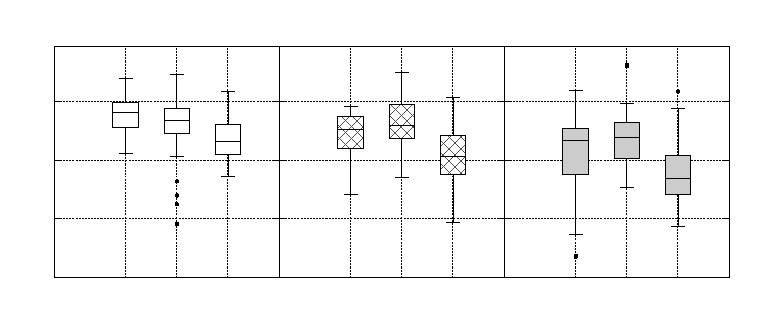
\includegraphics[width={360.00bp},height={144.00bp}]{Fat_latency}}%
    \gplfronttext
  \end{picture}%
\endgroup
}}
    \caption{fat-tree}
    \label{fig:latency:fat}
  \end{subfigure}
   \begin{subfigure}[b]{0.7\columnwidth}
    \resizebox{\textwidth}{!}{\footnotesize{% GNUPLOT: LaTeX picture with Postscript
\begingroup
  \fontfamily{Times-Roman}%
  \selectfont
  \makeatletter
  \providecommand\color[2][]{%
    \GenericError{(gnuplot) \space\space\space\@spaces}{%
      Package color not loaded in conjunction with
      terminal option `colourtext'%
    }{See the gnuplot documentation for explanation.%
    }{Either use 'blacktext' in gnuplot or load the package
      color.sty in LaTeX.}%
    \renewcommand\color[2][]{}%
  }%
  \providecommand\includegraphics[2][]{%
    \GenericError{(gnuplot) \space\space\space\@spaces}{%
      Package graphicx or graphics not loaded%
    }{See the gnuplot documentation for explanation.%
    }{The gnuplot epslatex terminal needs graphicx.sty or graphics.sty.}%
    \renewcommand\includegraphics[2][]{}%
  }%
  \providecommand\rotatebox[2]{#2}%
  \@ifundefined{ifGPcolor}{%
    \newif\ifGPcolor
    \GPcolortrue
  }{}%
  \@ifundefined{ifGPblacktext}{%
    \newif\ifGPblacktext
    \GPblacktexttrue
  }{}%
  % define a \g@addto@macro without @ in the name:
  \let\gplgaddtomacro\g@addto@macro
  % define empty templates for all commands taking text:
  \gdef\gplbacktext{}%
  \gdef\gplfronttext{}%
  \makeatother
  \ifGPblacktext
    % no textcolor at all
    \def\colorrgb#1{}%
    \def\colorgray#1{}%
  \else
    % gray or color?
    \ifGPcolor
      \def\colorrgb#1{\color[rgb]{#1}}%
      \def\colorgray#1{\color[gray]{#1}}%
      \expandafter\def\csname LTw\endcsname{\color{white}}%
      \expandafter\def\csname LTb\endcsname{\color{black}}%
      \expandafter\def\csname LTa\endcsname{\color{black}}%
      \expandafter\def\csname LT0\endcsname{\color[rgb]{1,0,0}}%
      \expandafter\def\csname LT1\endcsname{\color[rgb]{0,1,0}}%
      \expandafter\def\csname LT2\endcsname{\color[rgb]{0,0,1}}%
      \expandafter\def\csname LT3\endcsname{\color[rgb]{1,0,1}}%
      \expandafter\def\csname LT4\endcsname{\color[rgb]{0,1,1}}%
      \expandafter\def\csname LT5\endcsname{\color[rgb]{1,1,0}}%
      \expandafter\def\csname LT6\endcsname{\color[rgb]{0,0,0}}%
      \expandafter\def\csname LT7\endcsname{\color[rgb]{1,0.3,0}}%
      \expandafter\def\csname LT8\endcsname{\color[rgb]{0.5,0.5,0.5}}%
    \else
      % gray
      \def\colorrgb#1{\color{black}}%
      \def\colorgray#1{\color[gray]{#1}}%
      \expandafter\def\csname LTw\endcsname{\color{white}}%
      \expandafter\def\csname LTb\endcsname{\color{black}}%
      \expandafter\def\csname LTa\endcsname{\color{black}}%
      \expandafter\def\csname LT0\endcsname{\color{black}}%
      \expandafter\def\csname LT1\endcsname{\color{black}}%
      \expandafter\def\csname LT2\endcsname{\color{black}}%
      \expandafter\def\csname LT3\endcsname{\color{black}}%
      \expandafter\def\csname LT4\endcsname{\color{black}}%
      \expandafter\def\csname LT5\endcsname{\color{black}}%
      \expandafter\def\csname LT6\endcsname{\color{black}}%
      \expandafter\def\csname LT7\endcsname{\color{black}}%
      \expandafter\def\csname LT8\endcsname{\color{black}}%
    \fi
  \fi
    \setlength{\unitlength}{0.0500bp}%
    \ifx\gptboxheight\undefined%
      \newlength{\gptboxheight}%
      \newlength{\gptboxwidth}%
      \newsavebox{\gptboxtext}%
    \fi%
    \setlength{\fboxrule}{0.5pt}%
    \setlength{\fboxsep}{1pt}%
\begin{picture}(7200.00,2880.00)%
    \gplgaddtomacro\gplbacktext{%
      \csname LTb\endcsname%%
      \put(782,528){\makebox(0,0)[r]{\strut{}$1120$}}%
      \csname LTb\endcsname%%
      \put(782,1089){\makebox(0,0)[r]{\strut{}$1128$}}%
      \csname LTb\endcsname%%
      \put(782,1651){\makebox(0,0)[r]{\strut{}$1136$}}%
      \csname LTb\endcsname%%
      \put(782,2212){\makebox(0,0)[r]{\strut{}$1144$}}%
      \csname LTb\endcsname%%
      \put(1126,242){\rotatebox{25}{\makebox(0,0)[r]{\strut{}SCC}}}%
      \csname LTb\endcsname%%
      \put(1617,242){\rotatebox{25}{\makebox(0,0)[r]{\strut{}CU}}}%
      \csname LTb\endcsname%%
      \put(2107,242){\rotatebox{25}{\makebox(0,0)[r]{\strut{}RWC}}}%
    }%
    \gplgaddtomacro\gplfronttext{%
      \csname LTb\endcsname%%
      \put(137,1482){\rotatebox{-270}{\makebox(0,0){\strut{}Time (ms)}}}%
      \csname LTb\endcsname%%
      \put(1439,2701){\makebox(0,0){\strut{}Nimble}}%
    }%
    \gplgaddtomacro\gplbacktext{%
      \csname LTb\endcsname%%
      \put(2942,528){\makebox(0,0)[r]{\strut{}$2340$}}%
      \csname LTb\endcsname%%
      \put(2942,1089){\makebox(0,0)[r]{\strut{}$2348$}}%
      \csname LTb\endcsname%%
      \put(2942,1651){\makebox(0,0)[r]{\strut{}$2356$}}%
      \csname LTb\endcsname%%
      \put(2942,2212){\makebox(0,0)[r]{\strut{}$2364$}}%
      \csname LTb\endcsname%%
      \put(3286,242){\rotatebox{25}{\makebox(0,0)[r]{\strut{}SCC}}}%
      \csname LTb\endcsname%%
      \put(3777,242){\rotatebox{25}{\makebox(0,0)[r]{\strut{}CU}}}%
      \csname LTb\endcsname%%
      \put(4267,242){\rotatebox{25}{\makebox(0,0)[r]{\strut{}RWC}}}%
    }%
    \gplgaddtomacro\gplfronttext{%
      \csname LTb\endcsname%%
      \put(3599,2701){\makebox(0,0){\strut{}SwingState}}%
    }%
    \gplgaddtomacro\gplbacktext{%
      \csname LTb\endcsname%%
      \put(5102,528){\makebox(0,0)[r]{\strut{}$1520$}}%
      \csname LTb\endcsname%%
      \put(5102,1089){\makebox(0,0)[r]{\strut{}$1532$}}%
      \csname LTb\endcsname%%
      \put(5102,1651){\makebox(0,0)[r]{\strut{}$1544$}}%
      \csname LTb\endcsname%%
      \put(5102,2212){\makebox(0,0)[r]{\strut{}$1556$}}%
      \csname LTb\endcsname%%
      \put(5446,242){\rotatebox{25}{\makebox(0,0)[r]{\strut{}SCC}}}%
      \csname LTb\endcsname%%
      \put(5937,242){\rotatebox{25}{\makebox(0,0)[r]{\strut{}CU}}}%
      \csname LTb\endcsname%%
      \put(6427,242){\rotatebox{25}{\makebox(0,0)[r]{\strut{}RWC}}}%
    }%
    \gplgaddtomacro\gplfronttext{%
      \csname LTb\endcsname%%
      \put(5759,2701){\makebox(0,0){\strut{}OpenNF}}%
    }%
    \gplbacktext
    \put(0,0){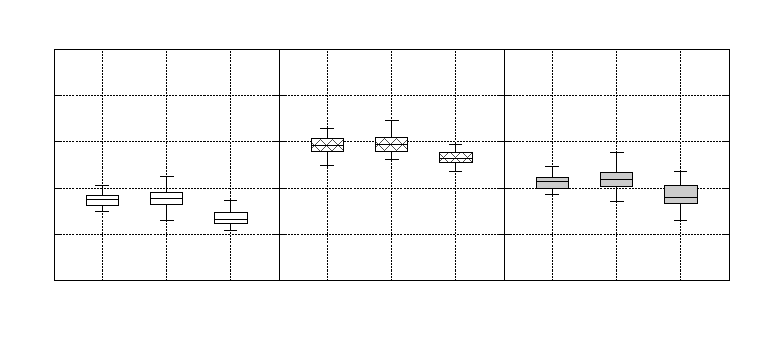
\includegraphics[width={360.00bp},height={144.00bp}]{Forthnet_latency}}%
    \gplfronttext
  \end{picture}%
\endgroup
}}
    \caption{Forthnet}
    \label{fig:latency:forthnet}
  \end{subfigure}
\caption{Times for receiving $10\megabytes$ upon link failure}
\label{fig:latency}
\end{figure}